\RCSdef{\ArrangementOnSurfaceRev}{$Id$}
\RCSdefDate{\ArrangementOnSurfaceDate}{$Date$}

\ccParDims

\ccUserChapter{2D Arrangements}

\begingroup

\label{chapterArrangement_on_surface_2}
\ccChapterRelease{\ArrangementOnSurfaceRev. \ \ArrangementOnSurfaceDate}
\ccChapterAuthor{Ron Wein \and Eric Berberich \and Efi Fogel \and Dan Halperin \and Michael Hemmer \and Oren Salzman \and Baruch Zukerman}


\begin{ccPkgDescription}{3D Convex Hulls\label{Pkg:ConvexHull3}}
\ccPkgHowToCiteCgal{cgal:hs-ch3-07}
\ccPkgSummary{This package provides functions 
for computing convex hulls in three dimensions as well as functions
for checking if sets of points are strongly convex are not. One can
compute the convex hull of a set of points in three dimensions in one
of three ways: using a static algorithm, using an incremental
construction algorithm, or using a triangulation to get a fully
dynamic computation.}

\ccPkgDependsOn{All algorithms produce as output a \ccRef[3D Polyhedron]{Pkg:Polyhedron}. 
                The dynamic algorithms depend on \ccRef[3D Triangulations]{Pkg:Triangulation3}}
\ccPkgIntroducedInCGAL{1.1}
\ccPkgLicense{\ccLicenseQPL}
\ccPkgIllustration{Convex_hull_3/bunny.png}{Convex_hull_3/bunny.png}
\end{ccPkgDescription}


\minitoc

\lcTex{%
  \newlength{\ArrangementTwoWidthExtra}\setlength{\ArrangementTwoWidthExtra}{1.1cm}
  \newlength{\ArrangementTwoWidthLineReal}\setlength{\ArrangementTwoWidthLineReal}{\linewidth}
  \addtolength{\ArrangementTwoWidthLineReal}{-\ArrangementTwoWidthExtra}
  \newlength{\ArrangementTwoMinipageSpace}\setlength{\ArrangementTwoMinipageSpace}{0.2cm}

  \newlength{\ArrangementTwoWidthLeft}
  \newlength{\ArrangementTwoWidthRight}
}

\newcommand{\calC}{{\cal C}}
\newcommand{\calA}{{\cal A}}
\newcommand{\dcel}{{\sc Dcel}}
\newcommand{\kdtree}{{\sc Kd}-tree}

\lcTex{%
\ifpdf
  \pdfstringdefDisableCommands{
    \def\dcel{DCEL}
  }
\fi%
}

\section{Introduction\label{arr_sec:intro}}
% ===================

Given a set $\calC$ of planar curves, the {\em arrangement}
$\calA(\calC)$ is the subdivision of the plane into zero-dimensional,
one-dimensional and two-dimensional cells, called {\em vertices}, {\em
edges} and {\em faces}, respectively induced by the curves in $\calC$.
Arrangements are ubiquitous in the computational-geometry
literature and have many applications;
see, e.g.,~\cite{as-aa-00}, \cite{cgal:h-a-04}.

The curves in $\calC$ can intersect each other (a single curve may also
be self-intersecting or may be comprised of several disconnected branches)
and are not necessarily $x$-monotone.\footnote{A continuous planar curve $C$
is {\em $x$-monotone} if every vertical line intersects it at
most once. For example, a non-vertical line segment is always
$x$-monotone and so is the graph of any continuous function $y = f(x)$.
For convenience, we treat vertical line segments as {\em weakly
$x$-monotone}, as there exists a single vertical line that overlaps them.
A circle of radius $r$ centered at $(x_0, y_0)$ is not $x$-monotone, as
the vertical line $x = x_0$ intersects it at $(x_0, y_0 - r)$ and at
$(x_0, y_0 + r)$.}
We construct a collection $\calC''$ of
$x$-monotone subcurves that are pairwise disjoint in their interiors
in two steps as follows. First, we decompose each curve in $\calC$
into maximal $x$-monotone subcurves (and possibly isolated points),
obtaining the collection $\calC'$. Note that an $x$-monotone curve cannot
be self-intersecting. Then, we decompose each curve in $\calC'$ into
maximal connected subcurves not intersecting any other
curve (or point) in $\calC'$. The collection $\calC''$ may also
contain isolated points, if the curves of $\calC$ contain such
points. The arrangement induced by the collection $\calC''$ can be
conveniently embedded as a planar graph, whose vertices are associated
with curve endpoints or with isolated points, and whose edges are
associated with subcurves. It is easy to see that
$\calA(\calC) = \calA(\calC'')$. This graph can be represented using a
{\em doubly-connected edge list} data-structure (\dcel\ for short),
which consists of containers of vertices, edges and faces and
maintains the incidence relations among these objects.

The main idea behind the \dcel\ data-structure is to represent
each edge using a pair of directed {\em halfedges}, one going from
the $xy$-lexicographically smaller (left) endpoint of the curve toward
its the $xy$-lexicographically larger (right) endpoint, and the other,
known as its {\em twin} halfedge, going in the opposite direction. As each
halfedge is directed, we say it has a {\em source} vertex and a {\em target}
vertex. Halfedges are used to separate faces, and to
connect vertices (with the exception of {\em isolated vertices}, which
are unconnected).

If a vertex $v$ is the target of a halfedge $e$, we say that $v$
and $e$ are {\em incident} to each other. The halfedges incident
to a vertex $v$ form a circular list oriented in a clockwise order
around this vertex. (An isolated vertex has no incident halfedges.)

Each halfedge $e$ stores a pointer to its {\it incident face},
which is the face lying to its left. Moreover, every halfedge is
followed by another halfedge sharing the same incident face, such
that the target vertex of the halfedge is the same as the source
vertex of the next halfedge. The halfedges are therefore connected
in circular lists, and form chains, such that all edges of a chain
are incident to the same face and wind along its boundary. We call
such a chain a {\em connected component of the boundary} (or {\em
CCB} for short).

The unique CCB of halfedges winding in a counterclockwise orientation
along a face boundary is referred to as the {\em outer CCB} of the
face. For the time being let us consider only arrangements of
bounded curves, such that exactly one unbounded face exists in every
arrangement. The unbounded face does not have an outer boundary. Any
other connected component of the boundary of the face is called a
{\em hole} (or {\em inner CCB}), and can be represented as a circular
chain of halfedges winding in a clockwise orientation around it.
Note that a hole does not necessarily correspond to a single face,
as it may have no area, or alternatively it may consist of several
connected faces. Every face can have several holes contained in its
interior (or no holes at all). In addition, every face may contain
isolated vertices in its interior. See Figure~\ref{arr_fig:seg_dcel}
for an illustration of the various \dcel\ features. For more details
on the \dcel\ data structure see~\cite[Chapter~2]{bkos-cgaa-00}.

\begin{figure}[t]
\begin{ccTexOnly}
  \begin{center}
  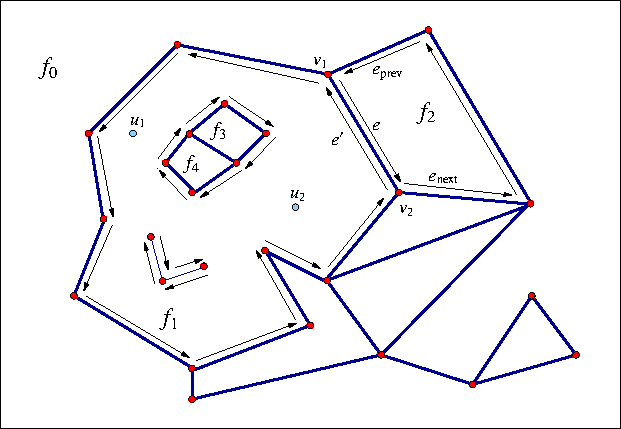
\includegraphics{Arrangement_on_surface_2/fig/arr_segs}
  \end{center}
\end{ccTexOnly}
\begin{ccHtmlOnly}
  <p><center>
  <img src="./fig/arr_segs.gif" border=0 alt="Arrangement of segments">
  </center>
\end{ccHtmlOnly}
\caption{An arrangement of interior-disjoint line segments with some
of the \dcel\ records that represent it. The unbounded face $f_0$ has
a single connected component that forms a hole inside it, and this hole
is comprised if several faces. The half-edge $e$ is directed from its
source vertex $v_1$ to its target vertex $v_2$. This edge, together with
its twin $e'$, correspond to a line segment that connects the points
associated with $v_1$ and $v_2$ and separates the face $f_1$ from $f_2$.
The predecessor $e_{\rm prev}$ and successor
$e_{\rm next}$ of $e$ are part of the chain that form the outer
boundary of the face $f_2$. The face $f_1$ has a more complicated
structure as it contains two holes in its interior: One hole
consists of two adjacent faces $f_3$ and $f_4$, while the other
hole is comprised of two edges. $f_1$ also contains two isolated
vertices $u_1$ and $u_2$ in its interior.\label{arr_fig:seg_dcel}}
\end{figure}

The $x$-monotone curves of an arrangement are embedded in an
rectangular two-dimensional area called the parameter
space.\footnote{The term parameter space stems from a major
  extension the arrangement package is going through to support
  arrangements embedded on certain two-dimensional parametric
  surfaces in three-dimensions (or higher).} The parameter space is
defined as $X \times Y$, where $X$ and $Y$ are open, half-open, or
closed intervals with endpoints in the compactified real line
$\mathbb{R} \cup \{-\infty,+\infty\}$. Let $b_l$, $b_r$, $b_b$, and
$b_t$ denote the endpoints of $X$ and $Y$, respectively. We
typically refer to these values as the left, right, bottom, and top
sides of the boundary of the parameter space. If the parameter space
is, for example, the entire compactified plane, which is currently
the only option supported by the package, $b_l = b_b = -\infty$ and
$b_r = b_t = +\infty$. 

The rest of this chapter is organized as follows: In
Section~\ref{arr_sec:arr_class} we review in detail the interface
of the \ccc{Arrangement_2} class-template, which is the central
component in the arrangement package. In
Section~\ref{arr_sec:queries} we show how queries on an arrangement
can be issued. In Section~\ref{arr_sec:gl_funcs} we
review some important free (global) functions that operate on
arrangements, the most important ones being the free 
insertion-functions. Section~\ref{arr_sec:traits} contains detailed
descriptions of the various geometric traits classes included in
the arrangement package. Using these traits classes it is possible
to construct arrangements of different families of curves. In
Section~\ref{arr_sec:notif} we review the notification mechanism
that allows external classes to keep track of the changes that an
arrangement instance goes through. Section~\ref{arr_sec:ex_dcel}
explains how to extend the \dcel\ records, to store extra data
with them, and to efficiently update this data.
In Section~\ref{arr_sec:overlay} we introduce the fundamental
operation of overlaying two arrangements.
Section~\ref{arr_sec:arr_with_hist} describes the
\ccc{Arrangement_with_history_2} class-template that extends the
arrangement by storing additional history records with its curves.
Finally, in Section~\ref{arr_sec:io} we review the arrangement
input/output functions.

\section{The Main Arrangement Class\label{arr_sec:arr_class}}
%===================================

The class \ccc{Arrangement_2<Traits,Dcel>} is the main class in
the arrangement package. It is used to represent planar
arrangements and provides the interface needed to construct them,
traverse them, and maintain them. An arrangement is defined by
a geometric {\em traits} class that determines the family of planar
curves that form the arrangement, and a \dcel\ class, which
represents the {\em topological structure} of the planar subdivision.
It supplies a minimal set of geometric operations (predicates and
constructions) required to construct and maintain the arrangement
and to operate on it.

The design of the arrangement package is guided by the need to
separate between the representation of the arrangements and the
various geometric algorithms that operate on them, and by the need to
separate between the topological and geometric aspects of the planar
subdivision. The separation is exhibited by the two template
parameters of the \ccc{Arrangement_2} template:
\begin{itemize}
\item The \ccc{Traits} template-parameter should be instantiated with
a model of the \ccc{ArrangementBasicTraits_2} concept. The traits
class defines the types of $x$-monotone curves and two-dimensional
points, \ccc{X_monotone_curve_2} and \ccc{Point_2} respectively, and
supports basic geometric predicates on them.

In the first sections of this chapter we always use
\ccc{Arr_segment_traits_2} as our traits class, to construct
arrangements of line segments. However, the arrangement package 
contains several other traits classes that can handle also
polylines (continuous piecewise-linear curves), conic arcs, and arcs
of rational functions. We exemplify the usage of these traits classes
in Section~\ref{arr_sec:traits}.
\item The \ccc{Dcel} template-parameter should be instantiated with
a class that is a model of the \ccc{ArrangementDcel} concept. The
value of this parameter is \ccc{Arr_default_dcel<Traits>} by default.
However, in many applications it is necessary
to extend the \dcel\ features; see Section~\ref{arr_sec:ex_dcel} for
further explanations and examples.
\end{itemize}

\subsection{A Simple Program}
%----------------------------

\lcTex{%
  \setlength{\ArrangementTwoWidthRight}{1.6cm}
  \setlength{\ArrangementTwoWidthLeft}{\ArrangementTwoWidthLineReal}
  \addtolength{\ArrangementTwoWidthLeft}{-\ArrangementTwoWidthRight}
  \begin{minipage}{\ArrangementTwoWidthLeft}
}
\begin{ccHtmlOnly}
  <p><center>
    <img src="./fig/triangle.gif" border=0 alt="triangle" align=right>
  </center>
\end{ccHtmlOnly}
The simple program listed below constructs a planar map of three line
segments forming a triangle. The constructed arrangement is instantiated
with the \ccc{Arr_segment_traits_2} traits class to handle segments only.
The resulting arrangement consists of two faces, a bounded triangular face
and the unbounded face.
The program is not very useful as it is, since it ends immediately
after the arrangement is constructed. We give more enhanced examples
in the rest of this chapter.
\lcTex{%
  \end{minipage}\hspace{\ArrangementTwoMinipageSpace}
  \begin{minipage}{\ArrangementTwoWidthRight}
    \begin{center}
    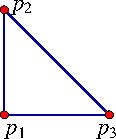
\includegraphics{Arrangement_2/fig/triangle}
    \end{center}
  \end{minipage}
}

\begin{alltt}
#include <CGAL/Cartesian.h>
#include <CGAL/MP_Float.h>
#include <CGAL/Quotient.h>
#include <CGAL/Arr_segment_traits_2.h>
#include <CGAL/Arrangement_2.h>

typedef CGAL::Quotient<CGAL::MP_Float>     Number_type;
typedef CGAL::Cartesian<Number_type>       Kernel;
typedef CGAL::Arr_segment_traits_2<Kernel> Traits_2;
typedef Traits_2::Point_2                  Point_2;
typedef Traits_2::X_monotone_curve_2       Segment_2;
typedef CGAL::Arrangement_2<Traits_2>      Arrangement_2;

int main()
\{
  Arrangement_2   arr;
  Segment_2       cv[3];
  Point_2         p1 (0, 0), p2 (0, 4), p3 (4, 0);
 
  cv[0] = Segment_2 (p1, p2);
  cv[1] = Segment_2 (p2, p3);
  cv[2] = Segment_2 (p3, p1);
  insert (arr, &cv[0], &cv[3]);

  return (0);
\}
\end{alltt}

\subsection{Traversing the Arrangement\label{arr_ssec:traverse}}
%--------------------------------------

The simplest and most fundamental arrangement operations are the
various traversal methods, which allow users to systematically go
over the relevant features of the arrangement at hand.

As mentioned above, the arrangement is represented as a \dcel,
which stores three containers of vertices, halfedges and faces. Thus,
the \ccc{Arrangement_2} class supplies iterators for these
containers. For example, the methods \ccc{vertices_begin()} and
\ccc{vertices_end()} return \ccc{Arrangement_2::Vertex_iterator}
objects that define the valid range of arrangement vertices. The value
type of this iterator is \ccc{Arrangement_2::Vertex}. Moreover, the
vertex-iterator type is equivalent to
\ccc{Arrangement_2::Vertex_handle}, which serves as a pointer to a
vertex. As we show next, all functions related to arrangement features
accept handle types as input parameters and return handle types as
their output.

In addition to the iterators for arrangement vertices, halfedges
and faces, the arrangement class also provides \ccc{edges_begin()}
and \ccc{edges_end()} that return
\ccc{Arrangement_2::Edge_iterator} objects for traversing the
arrangement edges. Note that the value type of this iterator is
\ccc{Arrangement_2::Halfedge}, representing one of the twin
halfedges that represent the edge.

All iterator, circulator\footnote{A {\em circulator} is used to
traverse a circular list, such as the list of halfedges incident to
a vertex --- see below.} and handle types also have non-mutable
({\em const}) counterparts. These non-mutable iterators are useful
to traverse an arrangement without changing it. For example,
the arrangement has a
non-constant member function called \ccc{vertices_begin()} that
returns a \ccc{Vertex_iterator} object and another const member
function that returns a \ccc{Vertex_const_iterator} object. In fact,
all methods listed in this section that return an iterator, a
circulator or a handle have non-mutable counterparts. It should be
noted that, for example, \ccc{Vertex_handle} can be readily converted
into a \ccc{Vertex_const_handle}, but not vice-verse.

Conversion of a non-mutable handle to a corresponding mutable
handle are nevertheless possible, and can be performed using the
static function \ccc{Arrangement_2::non_const_handle()} (see, e.g.,
Section~\ref{arr_ssec:pl}). There are
three variant of this function, one for each type of handle.

\subsubsection{Traversal Methods for an Arrangement Vertex\label{arr_sssec:tr_vertex}}
%~~~~~~~~~~~~~~~~~~~~~~~~~~~~~~~~~~~~~~~~~~~~~~~~~~~~~~~~~~

A vertex is always associated with a geometric entity, namely with
a \ccc{Point_2} object, which can be obtained by the \ccc{point()}
method of the \ccc{Vertex} class nested within \ccc{Arrangement_2}.

The \ccc{is_isolated()} method determines whether a vertex is isolated
or not. Recall that the halfedges incident to a non-isolated vertex,
namely the halfedges that share a common target vertex, form a circular
list around this vertex. The \ccc{incident_halfedges()} method returns
a circulator of type \ccc{Arrangement_2::Halfedge_around_vertex_circulator}
that enables the traversal of this circular list in a clockwise
direction. The value type of this circulator is \ccc{Halfedge}.

The following function prints all the neighbors of a given
arrangement vertex (assuming that the \ccc{Point_2} type can be
inserted into the standard output using the \ccc{<<} operator). The
arrangement type is the same as in the simple example above.
\begin{alltt}
void print_neighboring_vertices (Arrangement_2::Vertex_const_handle v)
\{
  if (v->is_isolated()) \{
    std::cout << "The vertex (" << v->point() << ") is isolated" << std::endl;
    return;
  \}

  Arrangement_2::Halfedge_around_vertex_const_circulator first, curr;
  first = curr = v->incident_halfedges();

  std::cout << "The neighbors of the vertex (" << v->point() << ") are:";
  do \{
    // Note that the current halfedge is directed from u to v:
    Arrangement_2::Vertex_const_handle u = curr->source();
    std::cout << " (" << u->point() << ")";
  \} while (++curr != first);
  std::cout << std::endl;
\}
\end{alltt}

In case of an isolated vertex, it is possible to obtain the face
that contains this vertex using the \ccc{face()} method.

\subsubsection{Traversal Methods for an Arrangement Halfedge\label{arr_sssec:tr_halfedge}}
%~~~~~~~~~~~~~~~~~~~~~~~~~~~~~~~~~~~~~~~~~~~~~~~~~~~~~~~~~~~~

Each arrangement edge, realized as a pair of twin halfedges,
is associated with an \ccc{X_monotone_curve_2} object, which
can be obtained by the \ccc{curve()} method of the \ccc{Halfedge}
class nested in the \ccc{Arrangement_2} class.

The \ccc{source()} and \ccc{target()} methods return handles to
the halfedge source and target vertices respectively. We can
obtain a handle to the twin halfedge using the \ccc{twin()}
method. From the definition of halfedges, it follows that if
\ccc{he} is a halfedge handle, then:
\begin{itemize}
\item \ccc{he->curve()} is equivalent to \ccc{he->twin()->curve()},
\item \ccc{he->source()} is equivalent to \ccc{he->twin()->target()}, and
\item \ccc{he->target()} is equivalent to \ccc{he->twin()->source()}.
\end{itemize}

Every halfedge has an incident face that lies to its left, which
can be obtained by the \ccc{face()} method. Recall that a
halfedge is always one link in a connected chain of halfedges that
share the same incident face, known as a {\em CCB}. The
\ccc{prev()} and \ccc{next()} methods return handles to the
previous and next halfedges in the CCB respectively. 
%(note that \ccc{he->prev()} is not necessarily equivalent to
%\ccc{he->twin()->next()}).

As the CCB is a circular list of halfedges, it is only natural to 
traverse it using a circulator. The \ccc{ccb()} method returns a 
\ccc{Arrangement_2::Ccb_halfedge_circulator} object for the
halfedges along the CCB.

The function \ccc{print_ccb()} listed below prints all $x$-monotone
curves along a given CCB (assuming that the \ccc{Point_2} and the
\ccc{X_monotone_curve_2} types can be inserted into the standard output
using the \ccc{<<} operator).
\begin{alltt}
void print_ccb (Arrangement_2::Ccb_halfedge_const_circulator circ)
\{
  Ccb_halfedge_const_circulator curr = circ;
  std::cout << "(" << curr->source()->point() << ")";
  do \{
    Arrangement_2::Halfedge_const_handle he = curr->handle();
    std::cout << "   [" << he->curve() << "]   "
              << "(" << he->target()->point() << ")";
  \} while (++curr != circ);
  std::cout << std::endl;
\}
\end{alltt}

\subsubsection{Traversal Methods for an Arrangement Face\label{arr_sssec:tr_face}}
%~~~~~~~~~~~~~~~~~~~~~~~~~~~~~~~~~~~~~~~~~~~~~~~~~~~~~~~~

An arrangement of bounded curves always has a single unbounded face.
The function \ccc{unbounded_face()} returns a handle to this face.
(Note that an empty arrangement contains nothing {\em but} the
unbounded face.)

Given a \ccc{Face} object, we can use the \ccc{is_unbounded()}
method to determine whether it is unbounded. Bounded faces have an
outer CCB, and the \ccc{outer_ccb()} method returns a circulator
for the halfedges along this CCB. Note that the halfedges along
this CCB wind in a counterclockwise orientation around the outer
boundary of the face.

A face can also contain disconnected components in its interior,
namely holes and isolated vertices:
\begin{itemize}
\item The \ccc{holes_begin()} and \ccc{holes_end()} methods return
\ccc{Arrangement_2::Hole_iterator} iterators that define the range
of holes inside the face. The value type of this iterator is
\ccc{Ccb_halfedge_circulator}, defining the CCB that winds in a
clockwise orientation around a hole.
\item The \ccc{isolated_vertices_begin()} and
\ccc{isolated_vertices_end()} methods return
\ccc{Arrangement_2::Isolated_vertex_iterator} iterators that
define the range of isolated vertices inside the face. The value
type of this iterator is \ccc{Vertex}.
\end{itemize}

The function \ccc{print_face()} listed below prints the outer and
inner boundaries of a given face, using the function \ccc{print_ccb()},
which was introduced in the previous subsection.
\begin{alltt}
void print_face (Arrangement_2::Face_const_handle f)
\{
  // Print the outer boundary.
  if (f->is_unbounded())
    std::cout << "Unbounded face. " << std::endl;
  else \{
    std::cout << "Outer boundary: ";
    print_ccb (f->outer_ccb());
  \}

  // Print the boundary of each of the holes.
  Arrangement_2::Hole_const_iterator hi;
  int                                 index = 1;
  for (hi = f->holes_begin(); hi != f->holes_end(); ++hi, ++index) \{
    std::cout << "    Hole #" << index << ": ";
    print_ccb (*hi);
  \}

  // Print the isolated vertices.
  Arrangement_2::Isolated_vertex_const_iterator iv;
  for (iv = f->isolated_vertices_begin(), index = 1;
       iv != f->isolated_vertices_end(); ++iv, ++index)
  \{
    std::cout << "    Isolated vertex #" << index << ": "
              << "(" << iv->point() << ")" << std::endl;
  \}
\}
\end{alltt}

\subsubsection{Additional Example\label{arr_sssec:tr_ex}}
%~~~~~~~~~~~~~~~~~~~~~~~~~~~~~~~~~

The function listed below prints the current setting of a given
arrangement. This concludes the preview of the various traversal
methods.\footnote{The file \ccc{arr_print.h}, which can be
found under the examples folder, includes this function and the
rest of the functions listed in this section. Over there they are
written in a more generic fashion, where the arrangement type
serves as a template parameter for these functions, so different
instantiations of the \ccc{Arrangement_2<Traits,Dcel>} template
can be provided to the same function templates.}
\begin{alltt}
void print_arrangement (const Arrangement_2& arr)
\{
  // Print the arrangement vertices.
  Vertex_const_iterator vit;
  std::cout << arr.number_of_vertices() << " vertices:" << std::endl;
  for (vit = arr.vertices_begin(); vit != arr.vertices_end(); ++vit) \{
    std::cout << "(" << vit->point() << ")";
    if (vit->is_isolated())
      std::cout << " - Isolated." << std::endl;
    else
      std::cout << " - degree " << vit->degree() << std::endl;
  \}

  // Print the arrangement edges.
  Edge_const_iterator eit;
  std::cout << arr.number_of_edges() << " edges:" << std::endl;
  for (eit = arr.edges_begin(); eit != arr.edges_end(); ++eit)
    std::cout << "[" << eit->curve() << "]" << std::endl;

  // Print the arrangement faces.
  Face_const_iterator fit;
  std::cout << arr.number_of_faces() << " faces:" << std::endl;
  for (fit = arr.faces_begin(); fit != arr.faces_end(); ++fit)
    print_face (fit);
\}
\end{alltt}

\subsection{Modifying the Arrangement\label{arr_ssec:modify}}
%-------------------------------------

In this section we review the various member functions of the
\ccc{Arrangement_2} class that allow users to modify the
topological structure of the arrangement by introducing new edges
or vertices, modifying them, or removing them.

The arrangement member-functions that insert new curves into the
arrangement, thus enabling the construction of a planar subdivision, are
rather specialized, as they require a-priori knowledge on the location of
the inserted curve. Indeed, for most purposes it is more convenient to
construct an arrangement using the free (global) insertion-functions.

\subsubsection{Inserting Non-Intersecting $x$-Monotone Curves\label{arr_sssec:mf_insert_cv}}
%~~~~~~~~~~~~~~~~~~~~~~~~~~~~~~~~~~~~~~~~~~~~~~~~~~~~~~~~~~~~~

The most important functions that allow users to modify the
arrangement, and perhaps the most frequently used ones, are the
specialized insertion functions of $x$-monotone curves whose
interior is disjoint from any other curve in the existing
arrangement and do not contain any vertex of the arrangement. In
addition, these function require that the location of the curve in the
arrangement is known.

The motivation behind these rather harsh restrictions on the nature of
the inserted curves is the decoupling of the topological arrangement
representation from the various algorithms that operate on it. While
the insertion of an $x$-monotone curve whose interior is disjoint from
all existing arrangement features is quite straightforward (as we show
next), inserting curves that intersect with the curves already inserted
into the arrangement is much more complicated and requires the
application of non-trivial geometric algorithms.
These insertion operations are therefore implemented as free functions
that operate on the arrangement and the inserted curve(s); see
Section~\ref{arr_sec:gl_funcs} for more details and
examples.\footnote{You may skip to Section~\ref{arr_sec:gl_funcs},
and return to this subsection at a later point in time.}

\begin{figure}[t]
\begin{ccTexOnly}
  \begin{center}
  \begin{tabular}{ccc}
    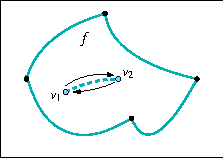
\includegraphics{Arrangement_2/fig/insert_in_face} &
    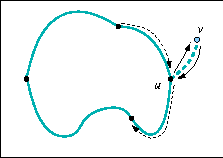
\includegraphics{Arrangement_2/fig/insert_from_vertex} &
    
\includegraphics{Arrangement_2/fig/insert_at_vertices}\\
  {\small (a)} & {\small (b)} & {\small (c)}\\
  \end{tabular}
  \end{center}
\end{ccTexOnly}
\begin{ccHtmlOnly}
  <p><center>
    <img src="./fig/insert.gif" border=0 alt="insert">
  </center>
\end{ccHtmlOnly}
\caption{The various specialized insertion procedures. The
inserted $x$-monotone curve is drawn with a light dashed line,
surrounded by two solid arrows that represent the pair of twin
half-edges added to the \dcel. Existing vertices are shown as
black dots while new vertices are shown as light dots. Existing
half-edges that are affected by the insertion operations are drawn
as dashed arrows. (a) Inserting a curve as a new hole inside the
face $f$. (b) Inserting a curve from an existing vertex $u$ that
corresponds to one of its endpoints. (c) Inserting an $x$-monotone
curve whose endpoints are the already existing vertices
$u_1$ and $u_2$. In our case, the new pair of half-edges close a
new face $f'$, where the hole $h_1$, which used to belong to $f$,
now becomes an enclave in this new face.} \label{arr_fig:insert}
\end{figure}

When an $x$-monotone curve is inserted into an existing arrangement, such
that the interior of this curve is disjoint from any arrangement feature,
only the following three scenarios are possible, depending on the status
of the endpoints of the inserted subcurve:
\begin{enumerate}
%
\item In case both curve endpoints do not correspond to any existing
arrangement vertex we have to create two new vertices
corresponding to the curve endpoints and connect them using a pair
of twin halfedges. This halfedge pair initiates a new hole inside
the face that contains the curve in its interior.
%
\item If exactly one endpoint corresponds to an existing arrangement
vertex (we distinguish between a vertex that corresponds to the left
endpoint of the inserted curve and a vertex corresponding to its right
endpoint), we have to create a new vertex that corresponds to the other
endpoint of the curve and to connect the two vertices by a pair of
twin halfedges that form an ``antenna'' emanating from the boundary
of an existing connected component (note that if the existing vertex
used to be isolated, this operation is actually equivalent to forming
a new hole inside the face that contains this vertex).

\lcTex{%
  \setlength{\ArrangementTwoWidthRight}{4.1cm}
  \setlength{\ArrangementTwoWidthLeft}{\ArrangementTwoWidthLineReal}
  \addtolength{\ArrangementTwoWidthLeft}{-\ArrangementTwoWidthRight}
  \begin{minipage}{\ArrangementTwoWidthLeft}
}
\item
\begin{ccHtmlOnly}
  <p><center>
    <img src="./fig/connect_comp.gif" border=0 alt="connect_comp" align=right>
  </center>
\end{ccHtmlOnly}
If both endpoints correspond to existing arrangement
vertices, we connect these vertices using a pair of twin halfedges.
(If one or both vertices are isolated this case reduces to one of
the two previous cases respectively.) The two following subcases may
occur:
\begin{itemize}
\item Two disconnected components are merged into a single connected
component (as is the case with the segment $s_1$ in the figure to the
left).
%
\item A new face is created, a face that splits from an existing
arrangement face. In this case we also have to examine the holes and
isolated vertices in the existing face and move the relevant ones
inside the new face (as is the case with the segment $s_2$ in the
figure to the left).
\end{itemize}
\lcTex{%
  \end{minipage}%\hspace{\ArrangementTwoMinipageSpace}
  \begin{minipage}{\ArrangementTwoWidthRight}
    \begin{center}\hspace{\ArrangementTwoMinipageSpace}
    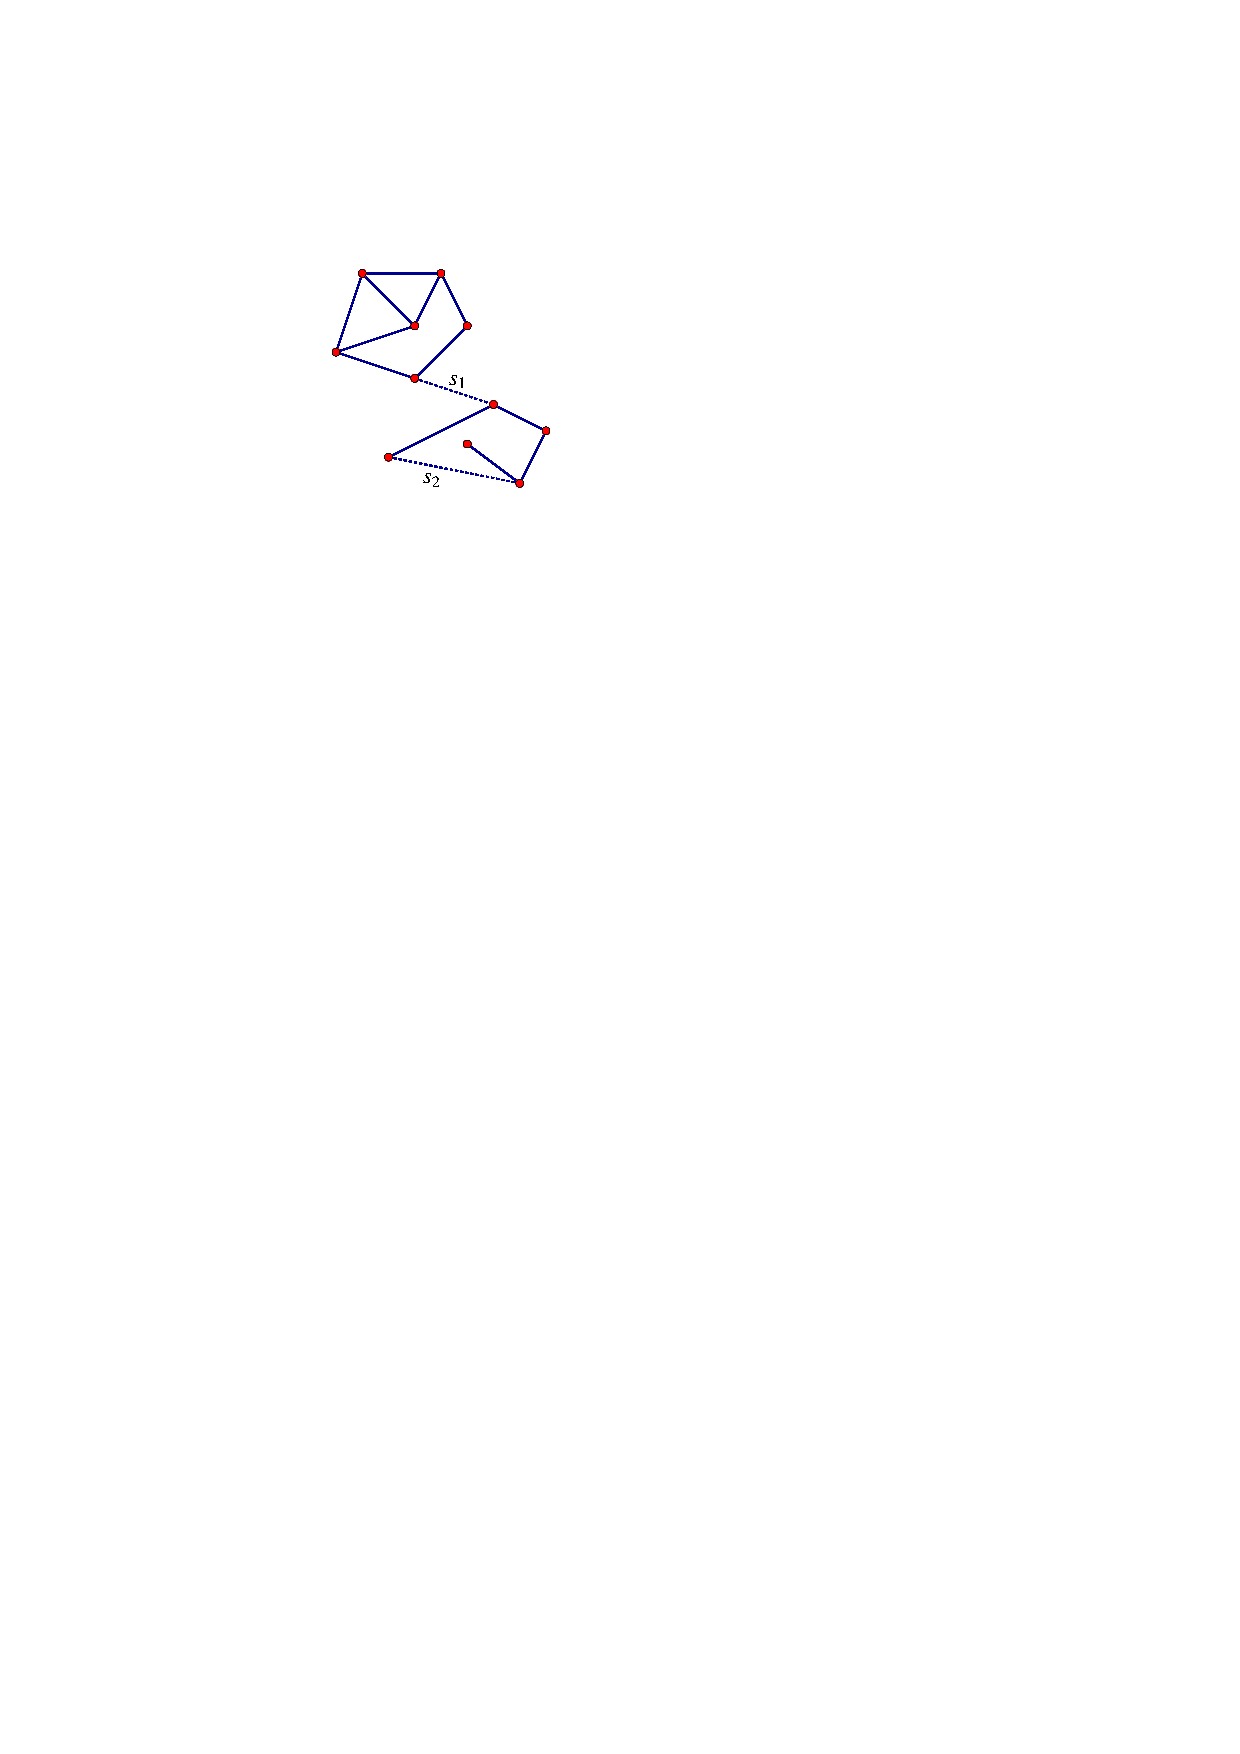
\includegraphics{Arrangement_2/fig/connect_comp}
    \end{center}
  \end{minipage}
}
\end{enumerate}

The \ccc{Arrangement_2} class offers insertion functions named
\ccc{insert_in_face_interior()}, \ccc{insert_from_left_vertex()},
\ccc{insert_from_right_vertex()} and \ccc{insert_at_vertices()}
that perform the special insertion procedures listed above. The
first function accepts an $x$-monotone curve $c$ and an arrangement
face $f$ that contains this curve in its interior. The other
functions accept an $x$-monotone curve $c$ and handles to the existing
vertices that correspond to the curve endpoint(s). Each of the four
functions returns a handle to one of the twin halfedges that have
been created, where:
\begin{itemize}
\item \ccc{insert_in_face_interior(c, f)} returns a halfedge directed
from the vertex corresponding to the left endpoint of \ccc{c}
toward the vertex corresponding to its right endpoint.
%
\item \ccc{insert_from_left_vertex(c, v)} and
\ccc{insert_from_right_vertex(c, v)} returns a halfedge whose
source is the vertex $v$ that and whose target is the new vertex
that has just been created.
%
\item \ccc{insert_at_vertices(c, v1, v2)} returns a halfedge directed
from $v_1$ to $v_2$.
\end{itemize}

\begin{figure}[t]
\begin{ccTexOnly}
  \begin{center}
  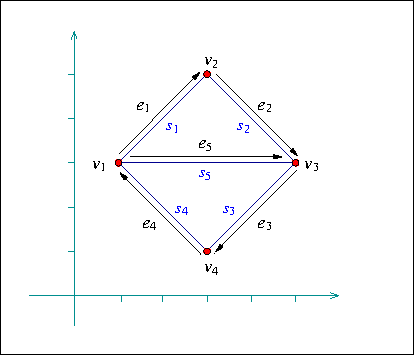
\includegraphics{Arrangement_2/fig/ex_1}
  \end{center}
\end{ccTexOnly}
\begin{ccHtmlOnly}
  <p><center>
  <img src="./fig/ex_1.gif" border=0 alt="Example 1">
  </center>
\end{ccHtmlOnly}
\caption{The arrangement of the line segments $s_1, \ldots, s_5$
constructed in \ccc{ex_edge_insertion.C}. The arrows mark the direction of
the halfedges returned from the various insertion
functions.\label{arr_fig:ex_1}}
\end{figure}

The following program demonstrates the usage of the four insertion
functions. It creates an arrangement of five line segments, as
depicted in Figure~\ref{arr_fig:ex_1}.\footnote{Notice that in all
figures in the rest of this chapter the coordinate axes are drawn
only for illustrative purposes and are {\em not} part of the
arrangement.} As the arrangement is very
simple, we use the simple Cartesian kernel of \cgal\ with integer
coordinates for the segment endpoints. We also use the 
\ccc{Arr_segment_traits_2} class that enables the efficient
maintenance of arrangements of line segments; see more details on
this traits class in Section~\ref{arr_sec:traits}. This example, as
many others in this chapter, uses some print-utility functions from
the file \ccc{print_arr.h}; these functions are also listed in
Section~\ref{arr_ssec:traverse}.

\ccIncludeExampleCode{../examples/Arrangement_2/ex_edge_insertion.cpp}

Observe that the first line segment is inserted in the interior of
the unbounded face. The other line segments are inserted
using the vertices created by the insertion of previous segments.
The resulting arrangement consists of three faces, where the two
bounded faces form together a hole in the unbounded face.

\subsubsection{Manipulating Isolated Vertices\label{arr_sssec:mf_iso_verts}}
%~~~~~~~~~~~~~~~~~~~~~~~~~~~~~~~~~~~~~~~~~~~~~~~~

Isolated points are in general simpler geometric entities than
curves and indeed the member functions that manipulate them are
easier to understand.

The function \ccc{insert_in_face_interior(p, f)} inserts an
isolated point $p$, located in the interior of a given face $f$,
into the arrangement and returns a handle to the arrangement
vertex it has created and associated with $p$. Naturally, this
function has a precondition that $p$ is really an isolated point,
namely it does not coincide with any existing arrangement vertex
and does not lie on any edge. As mentioned in
Section~\ref{arr_ssec:traverse}, it is possible to obtain the face
containing an isolated vertex handle $v$ by calling \ccc{v->face()}.

The function \ccc{remove_isolated_vertex(v)} receives a handle to
an isolated vertex and removes it from the arrangement.

\begin{figure}[t]
\begin{ccTexOnly}
  \begin{center}
  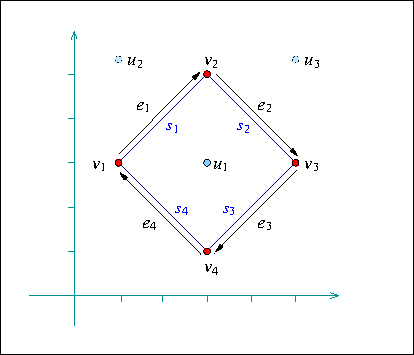
\includegraphics{Arrangement_2/fig/ex_2}
  \end{center}
\end{ccTexOnly}
\begin{ccHtmlOnly}
  <p><center>
  <img src="./fig/ex_2.gif" border=0 alt="Example 2">
  </center>
\end{ccHtmlOnly}
\caption{An arrangement of line segments containing three isolated
vertices, as constructed in \ccc{ex_isolated_vertices.C}. The vertices $u_2$
and $u_3$ are eventually removed from the arrangement.\label{arr_fig:ex_2}}
\end{figure}

The following program demonstrates the usage of the arrangement
member-functions for manipulating isolated vertices. It first
inserts three isolated vertices located inside the unbounded face, then
it inserts four line segments that form a rectangular hole inside the
unbounded face (see Figure~\ref{arr_fig:ex_2} for an
illustration). Finally, it traverses the vertices and removes those
isolated vertices that are still contained in the unbounded face
($u_2$ and $u_3$ in this case):

\ccIncludeExampleCode{../examples/Arrangement_2/ex_isolated_vertices.cpp}

\subsubsection{Manipulating Halfedges\label{arr_sssec:mf_halfedges}}
%~~~~~~~~~~~~~~~~~~~~~~~~~~~~~~~~~~~~~~~~~~~~~~~~

In the previous subsection we showed how to introduce new isolated
vertices in the arrangement. But how does one create a vertex that
lies on an existing arrangement edge (more precisely, on an
$x$-monotone curve that is associated with an arrangement edge)?

It should be noted that such an operation involves the splitting
of a curve at a given point in its interior, while the traits
class used by \ccc{Arrangement_2} does not necessarily have the
ability to perform such a split operation. However, if users have
the ability to split an $x$-monotone curve into two at a given point
$p$ (this is usually the case when employing a more sophisticated
traits class; see Section~\ref{arr_sec:traits} for more details)
they can use the \ccc{split_edge(e, c1, c2)} function, were
$c_1$ and $c_2$ are the two subcurves resulting from splitting the
$x$-monotone curve associated with the halfedge $e$ at some point
(call it $p$) in its interior. The function splits the halfedge pair into two
pairs, both incident to a new vertex $v$ associated with $p$, and
returns a handle to a halfedge whose source equals $e$'s source
vertex and whose target is the new vertex $v$.

The reverse operation is also possible. Suppose that we have a
vertex $v$ of degree $2$, whose two incident halfedges, $e_1$ and
$e_2$, are associated with the curves $c_1$ and $c_2$. Suppose
further that it is possible to merge these two curves into a single
continuous $x$-monotone curve $c$. Calling \ccc{merge_edge(e1, e2, c)}
will merge the two edges into a single edge associated with the curve
$c$, essentially removing the vertex $v$ from the arrangement.

Finally, the function \ccc{remove_edge(e)} removes the edge $e$
from the arrangement. Note that this operation is the reverse of
an insertion operation, so it may cause a connected
component to split into two, or two faces to merge into one, or a
hole to disappear. By default, if the removal of \ccc{e} causes one
of its end-vertices to become isolated, we remove this vertex as well.
However, users can control this behavior and choose to keep the
isolated vertices by supplying additional Boolean flags to
\ccc{remove_edge()} indicating whether the source and the target vertices
are to be removed should they become isolated.

\begin{figure}[t]
\begin{ccTexOnly}
  \begin{center}
  \begin{tabular}{ccc}
    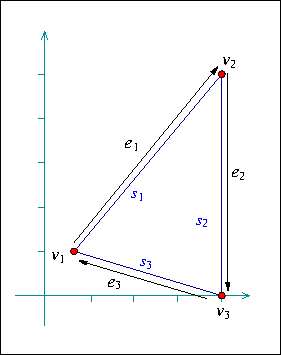
\includegraphics{Arrangement_2/fig/ex_3a} &
    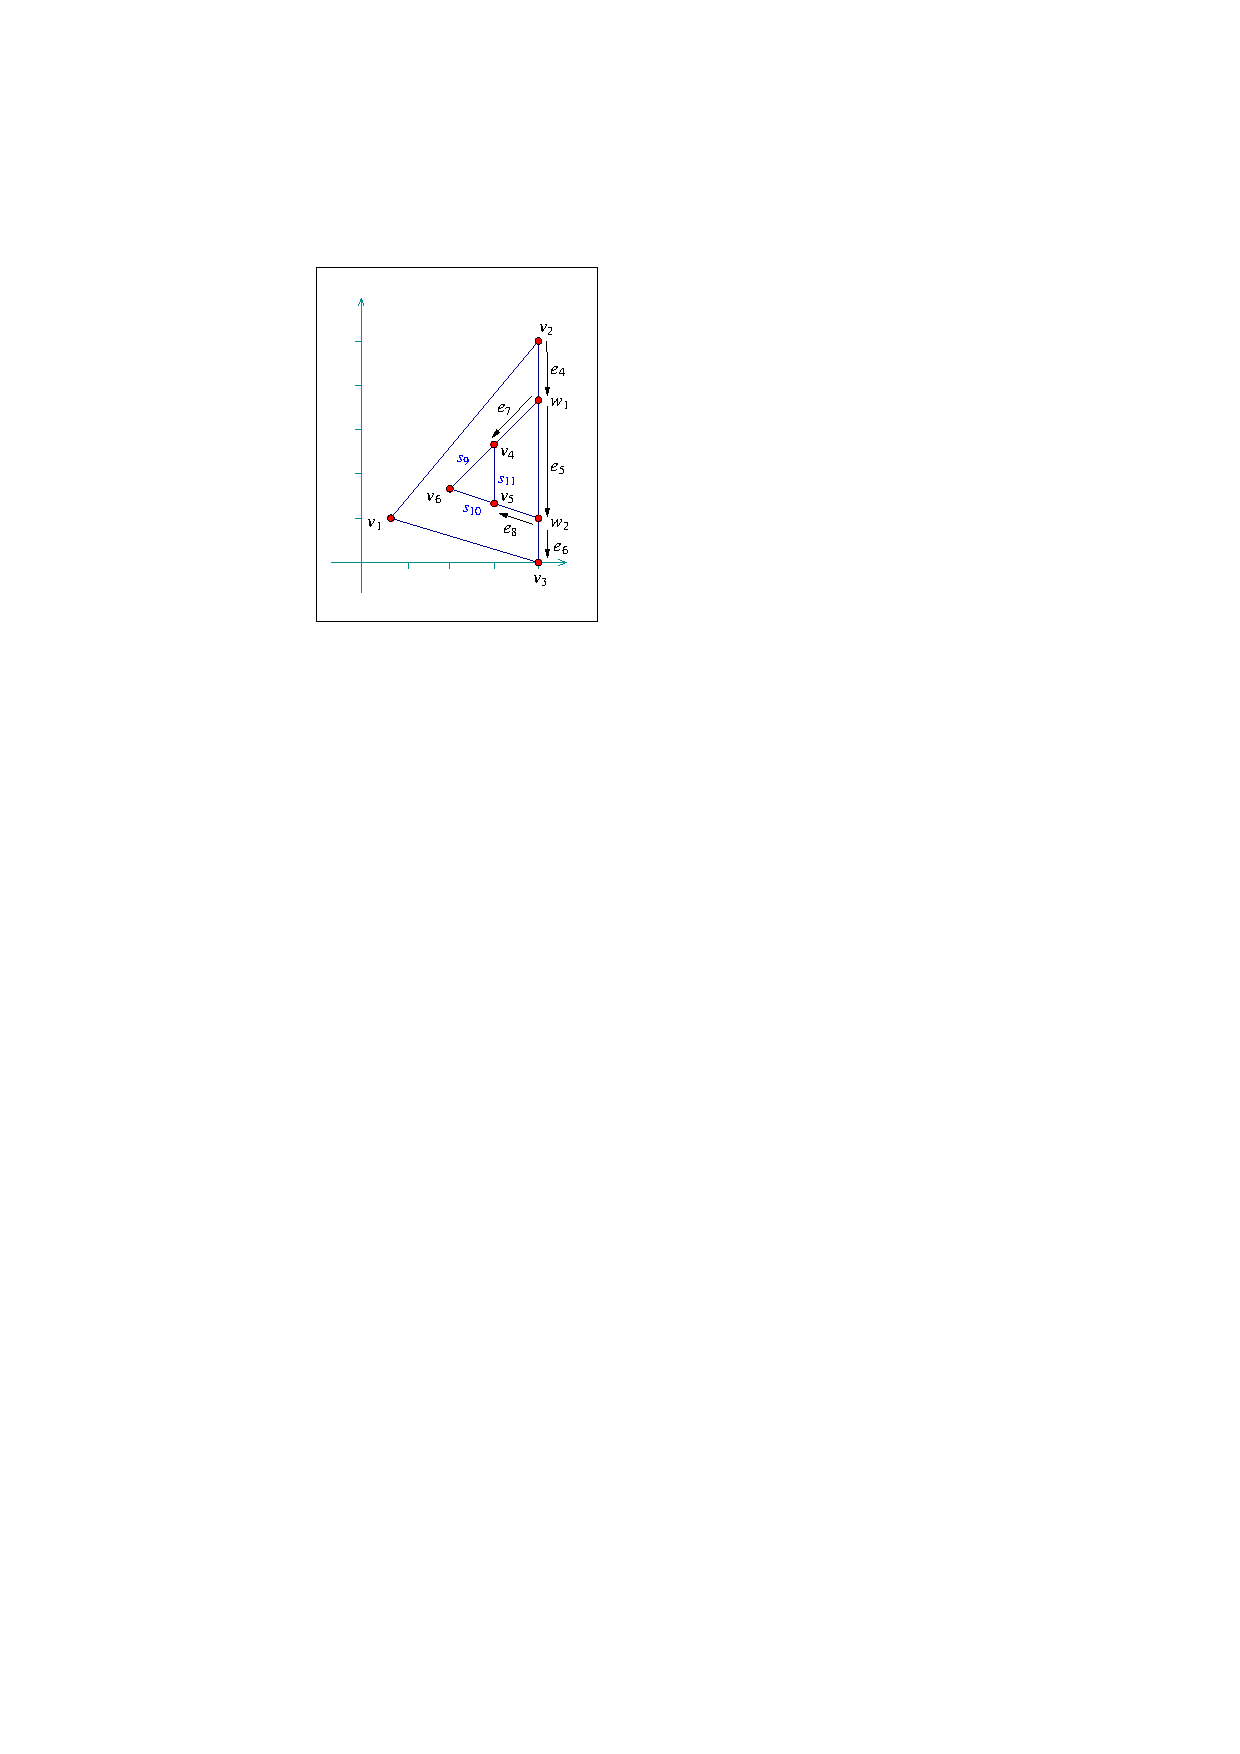
\includegraphics{Arrangement_2/fig/ex_3b} &
    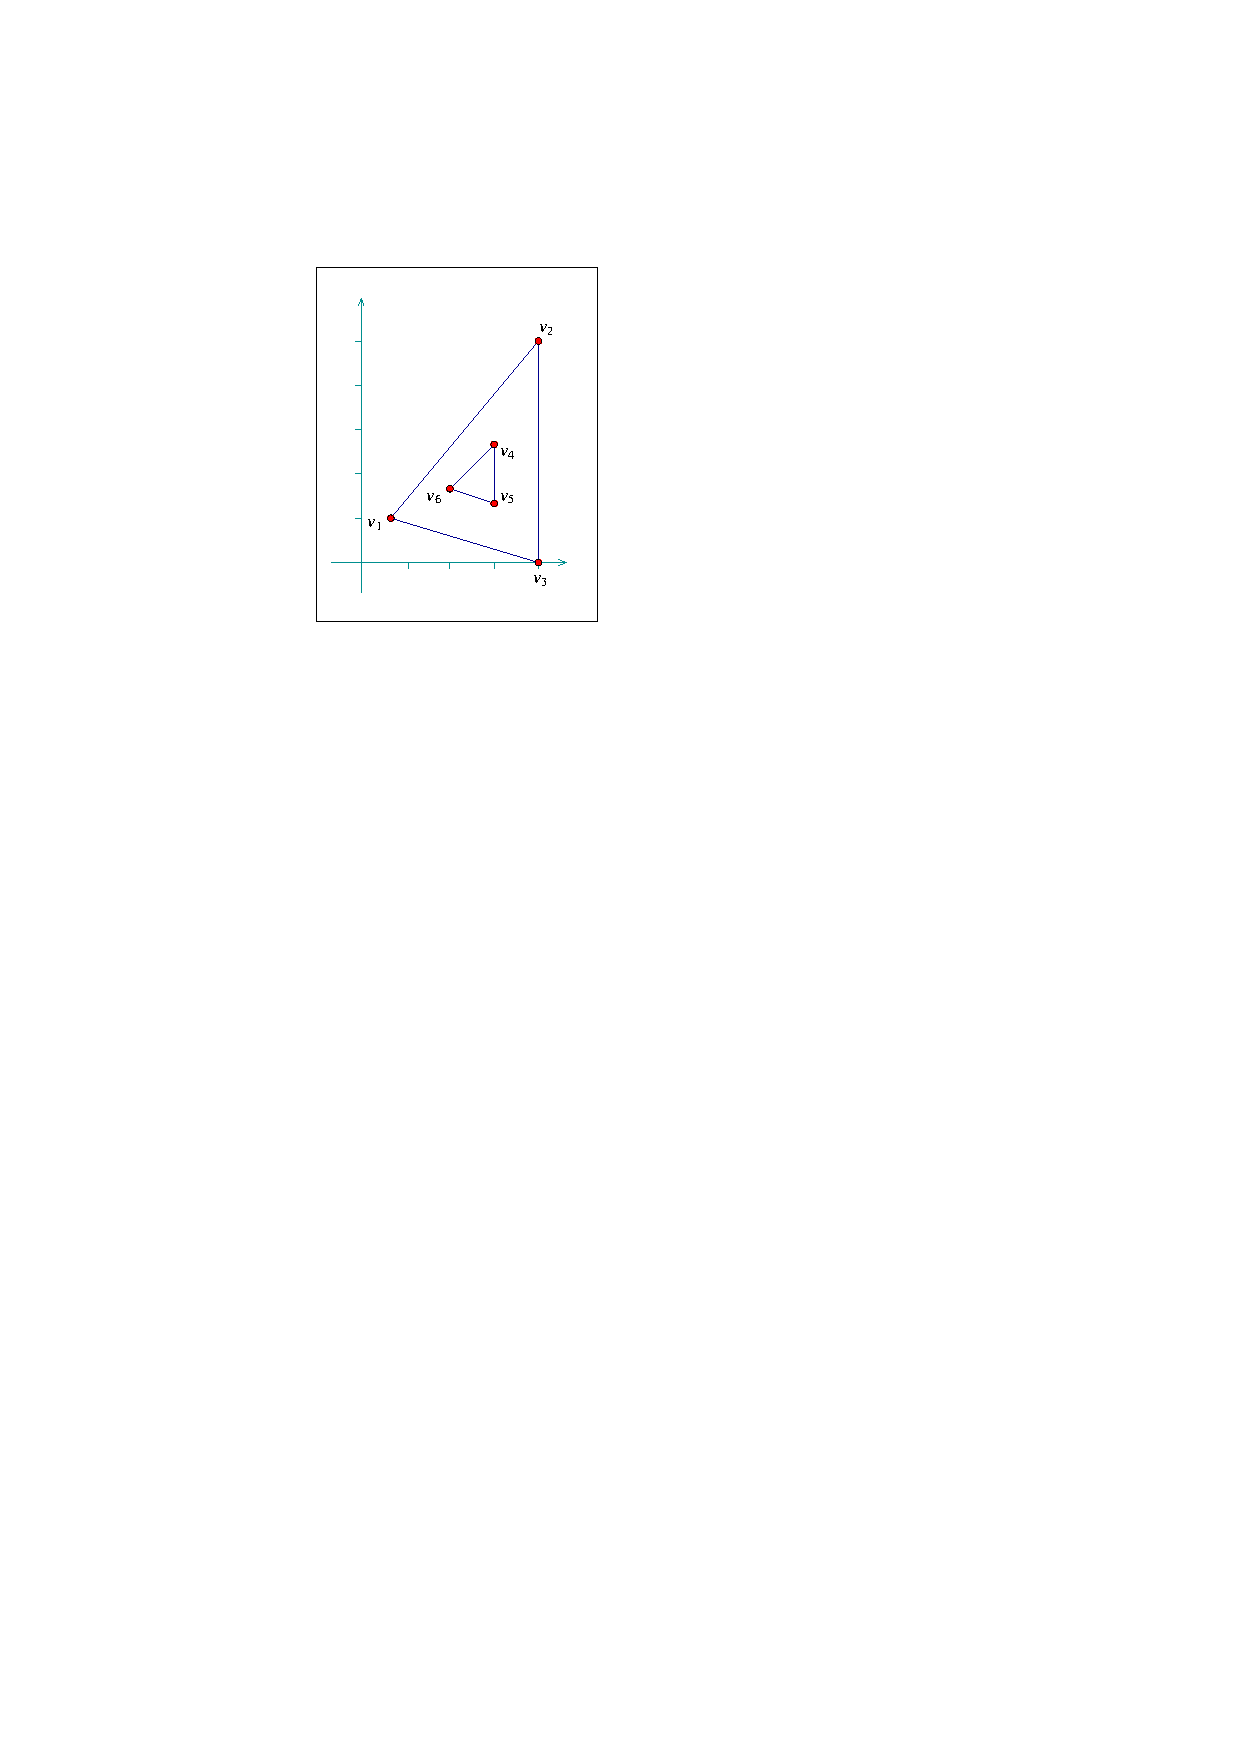
\includegraphics{Arrangement_2/fig/ex_3c} \\
  {\small (a)} & {\small (b)} & {\small (c)}\\
  \end{tabular}
  \end{center}
\end{ccTexOnly}
\begin{ccHtmlOnly}
  <p><center>
  <img src="./fig/ex_3.gif" border=0 alt="Example 3">
  </center>
\end{ccHtmlOnly}
\caption{An arrangement of line segments as constructed
in \ccc{ex_edge_manipulation.C}. Note that the edges $e_7$ and $e_8$ and the
vertices $w_1$ and $w_2$, introduced in step~(b) are eventually
removed in step~(c).\label{arr_fig:ex_3}}
\end{figure}

In the following example program we show how the edge-manipulation
functions can be used. The program works in three
steps, as demonstrated in Figure~\ref{arr_fig:ex_3}. Note that
here we still stick to integer coordinates, but as we work on a
larger scale we use an unbounded integer number-type (in this
case, the \ccc{Gmpz} type taken from the {\sc Gmp} library)
instead of the built-in \ccc{int} type.\footnote{As a rule of
thumb, one can use a bounded integer type for representing line
segments whose coordinates are bounded by
$\lfloor\sqrt[3]{M}\rfloor$, where $M$ is the maximal
representable integer value. This guarantees that no overflows
occur in the computations carried out by the traits class, hence
all traits-class predicates always return correct results.} 
In case the {\sc Gmp} library is not installed (as indicated by
the \ccc{CGAL_USE_GMP} flag defined in \ccc{CGAL/basic.h}), we
use \ccc{MP_Float}, a number-type included in \cgal's support
library that is capable of storing floating-point numbers with
unbounded mantissa. We also use the standard Cartesian
kernel of \cgal\ as our kernel. This is recommended when the
kernel is instantiated with a more complex number type, as we
demonstrate in other examples in this chapter.

\ccIncludeExampleCode{../examples/Arrangement_2/ex_edge_manipulation.cpp}

Note how we use the halfedge handles returned from
\ccc{split_edge()} and \ccc{merge_edge()}. Also note the insertion
of the isolated vertex $v_6$ located inside the triangular face (the
incident face of $e_7$). This vertex seizes from being isolated, as it
is gets connected to other vertices.

In this context, we should mention the two member functions
\ccc{modify_vertex(v, p)}, which sets $p$ to be the point
associated with the vertex $v$, and \ccc{modify_edge(e, c)}, which
sets $c$ to be the $x$-monotone curve associated with the halfedge
$e$. These functions have preconditions that $p$ is
geometrically equivalent to \ccc{v->point()} and $c$ is equivalent
to \ccc{e->curve()} (i.e., the two curves have the same graph),
respectively, to avoid the invalidation of the geometric structure of
the arrangement. At a first glance it may seen as these two functions
are of little use. However, we should keep in mind that there may be
extraneous data (probably non-geometric) associated with the point
objects or with the curve objects, as defined by the traits class. With
these two functions we can modify this data; see more details in
Section~\ref{arr_sec:traits}.

In addition, we can use these functions to replace a geometric
object (a point or a curve) with an equivalent object that has a
more compact representation. For example, we can replace the point
$(\frac{20}{40}, \frac{99}{33})$ associated with some vertex $v$,
by $(\frac{1}{2}, 3)$.

\newpage
\begin{ccAdvanced}
\subsubsection{Advanced Insertion Functions\label{arr_sssec:adv_insert}}
%~~~~~~~~~~~~~~~~~~~~~~~~~~~~~~~~~~~~~~~~~~~

\lcTex{%
  \setlength{\ArrangementTwoWidthRight}{2.5cm}
  \setlength{\ArrangementTwoWidthLeft}{\ArrangementTwoWidthLineReal}
  \addtolength{\ArrangementTwoWidthLeft}{-\ArrangementTwoWidthRight}
  \begin{minipage}{\ArrangementTwoWidthLeft}
}
\begin{ccHtmlOnly}
  <p><center>
    <img src="./fig/pred_around_vertex.gif" border=0 alt="pred_around_vertex" align=right>
  </center>
\end{ccHtmlOnly}
Assume that the specialized insertion function
\ccc{insert_from_left_vertex(c,v)} is invoked for a curve $c$,
whose left endpoint is already associated with a non-isolated
vertex $v$.  Namely, $v$ has already several incident halfedges. It
is necessary in this case to locate the exact place for the
new halfedge mapped to the inserted new curve $c$ in the circular
list of halfedges incident to $v$. More precisely, it is sufficient
to locate one of the halfedges \ccc{pred} directed toward $v$ such
that $c$ is located between \ccc{pred} and \ccc{pred->next()} in
clockwise order around $v$, in order to complete the insertion
(see Figure~\ref{arr_fig:insert} for an illustration). This may
take $O(d)$ time where $d$ is the degree of the vertex. However,
if the halfedge \ccc{pred} is known in advance, the insertion can
be carried out in constant time.
\lcTex{%
  \end{minipage}\hspace{\ArrangementTwoMinipageSpace}
  \begin{minipage}{\ArrangementTwoWidthRight}
    \begin{center}
    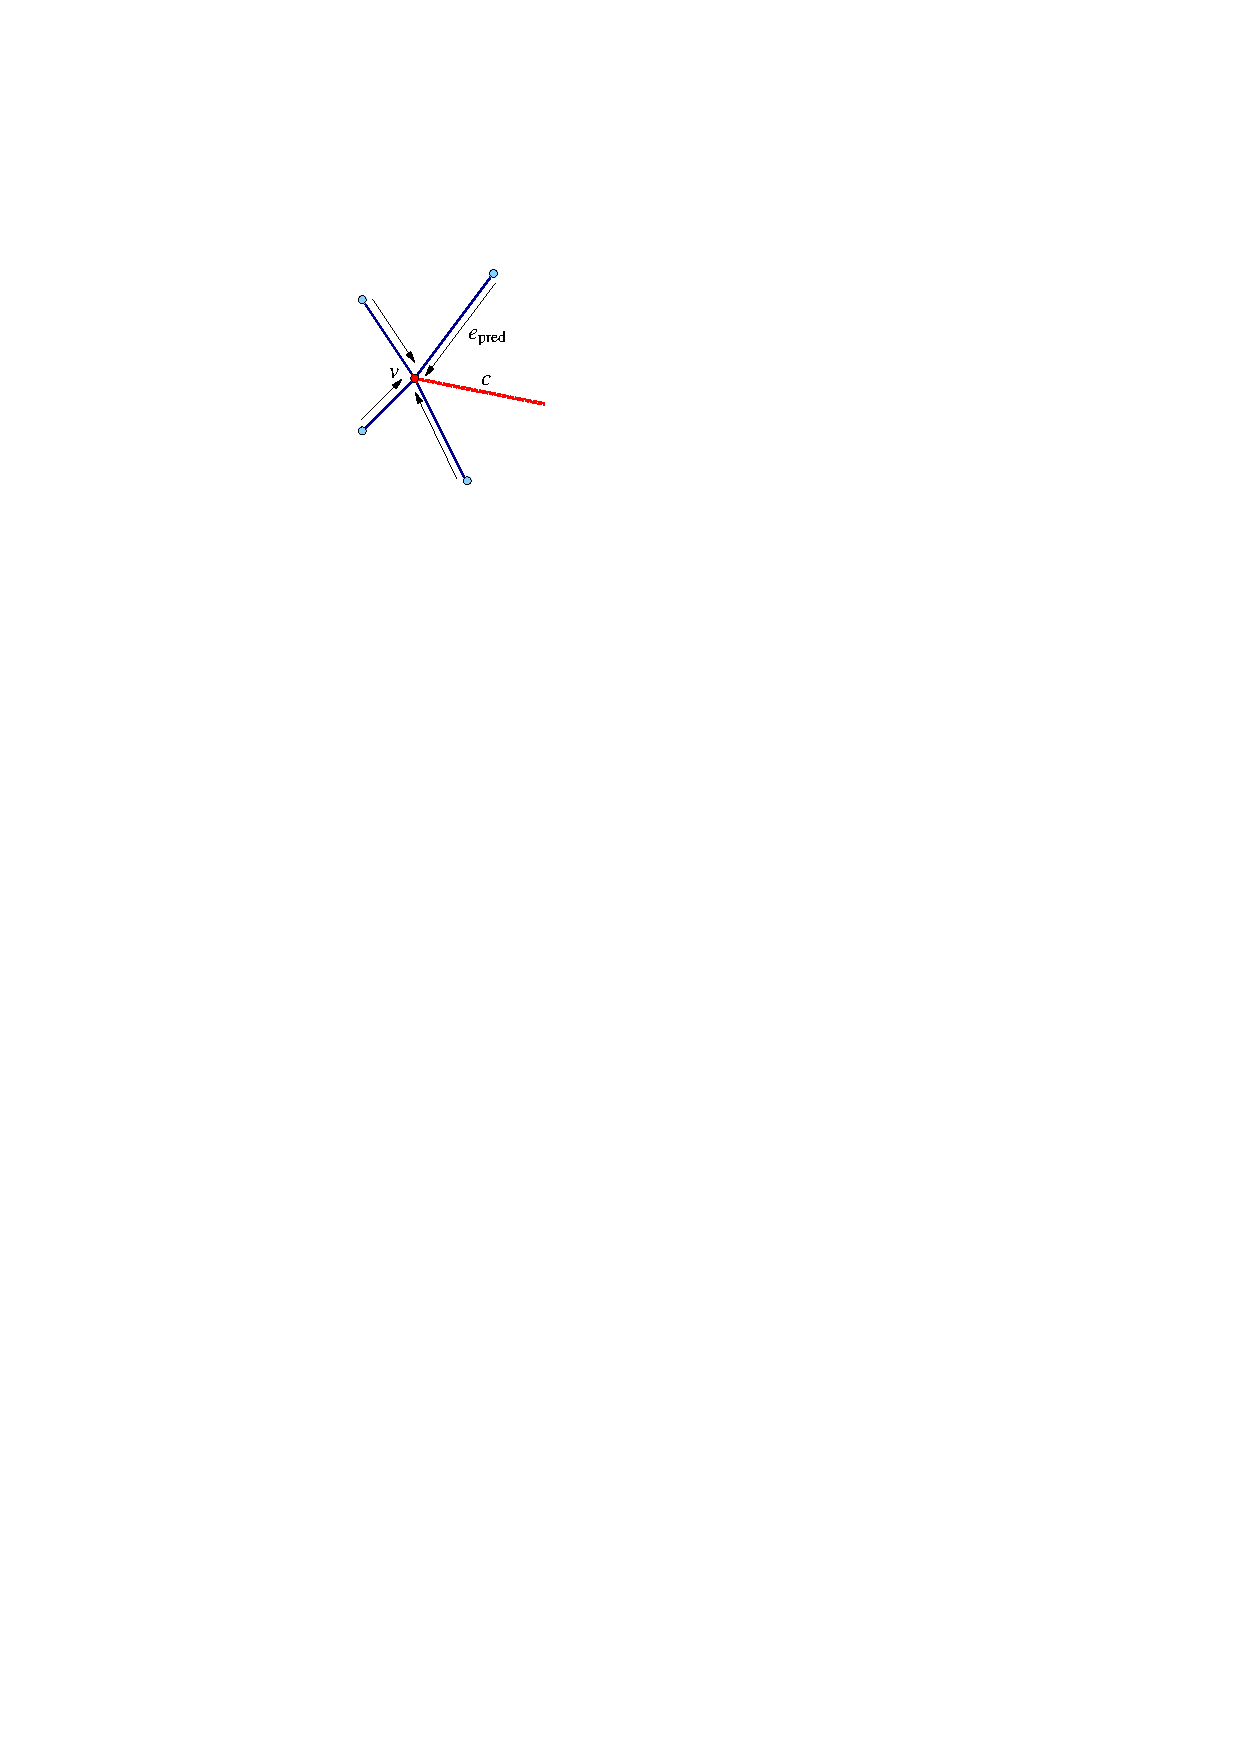
\includegraphics{Arrangement_2/fig/pred_around_vertex}
    \end{center}
  \end{minipage}
}

The \ccc{Arrangement_2} class provides the advanced versions of
the specialized insertion functions for a curve $c$ --- namely we have
\ccc{insert_from_left_vertex(c,pred)} and
\ccc{insert_from_right_vertex(c,pred)} that accept a halfedge \ccc{pred}
as specified above, instead of a vertex $v$. These functions are
more efficient, as they take constant time and do not perform any
geometric operations. Thus, they should be used when the halfedge
\ccc{pred} is known. In case that the vertex $v$ is isolated or
that the predecessor halfedge for the new inserted curve is not
known, the simpler versions of these insertion functions should be
used.

Similarly, there exist two overrides of the
\ccc{insert_at_vertices()} function: One that accept the two
predecessor halfedges around the two vertices $v_1$ and $v_2$ that
correspond to the curve endpoints, and one that accepts a handle
for one vertex and a predecessor halfedge around the other
vertex.

\begin{figure}[t]
\begin{ccTexOnly}
  \begin{center}
  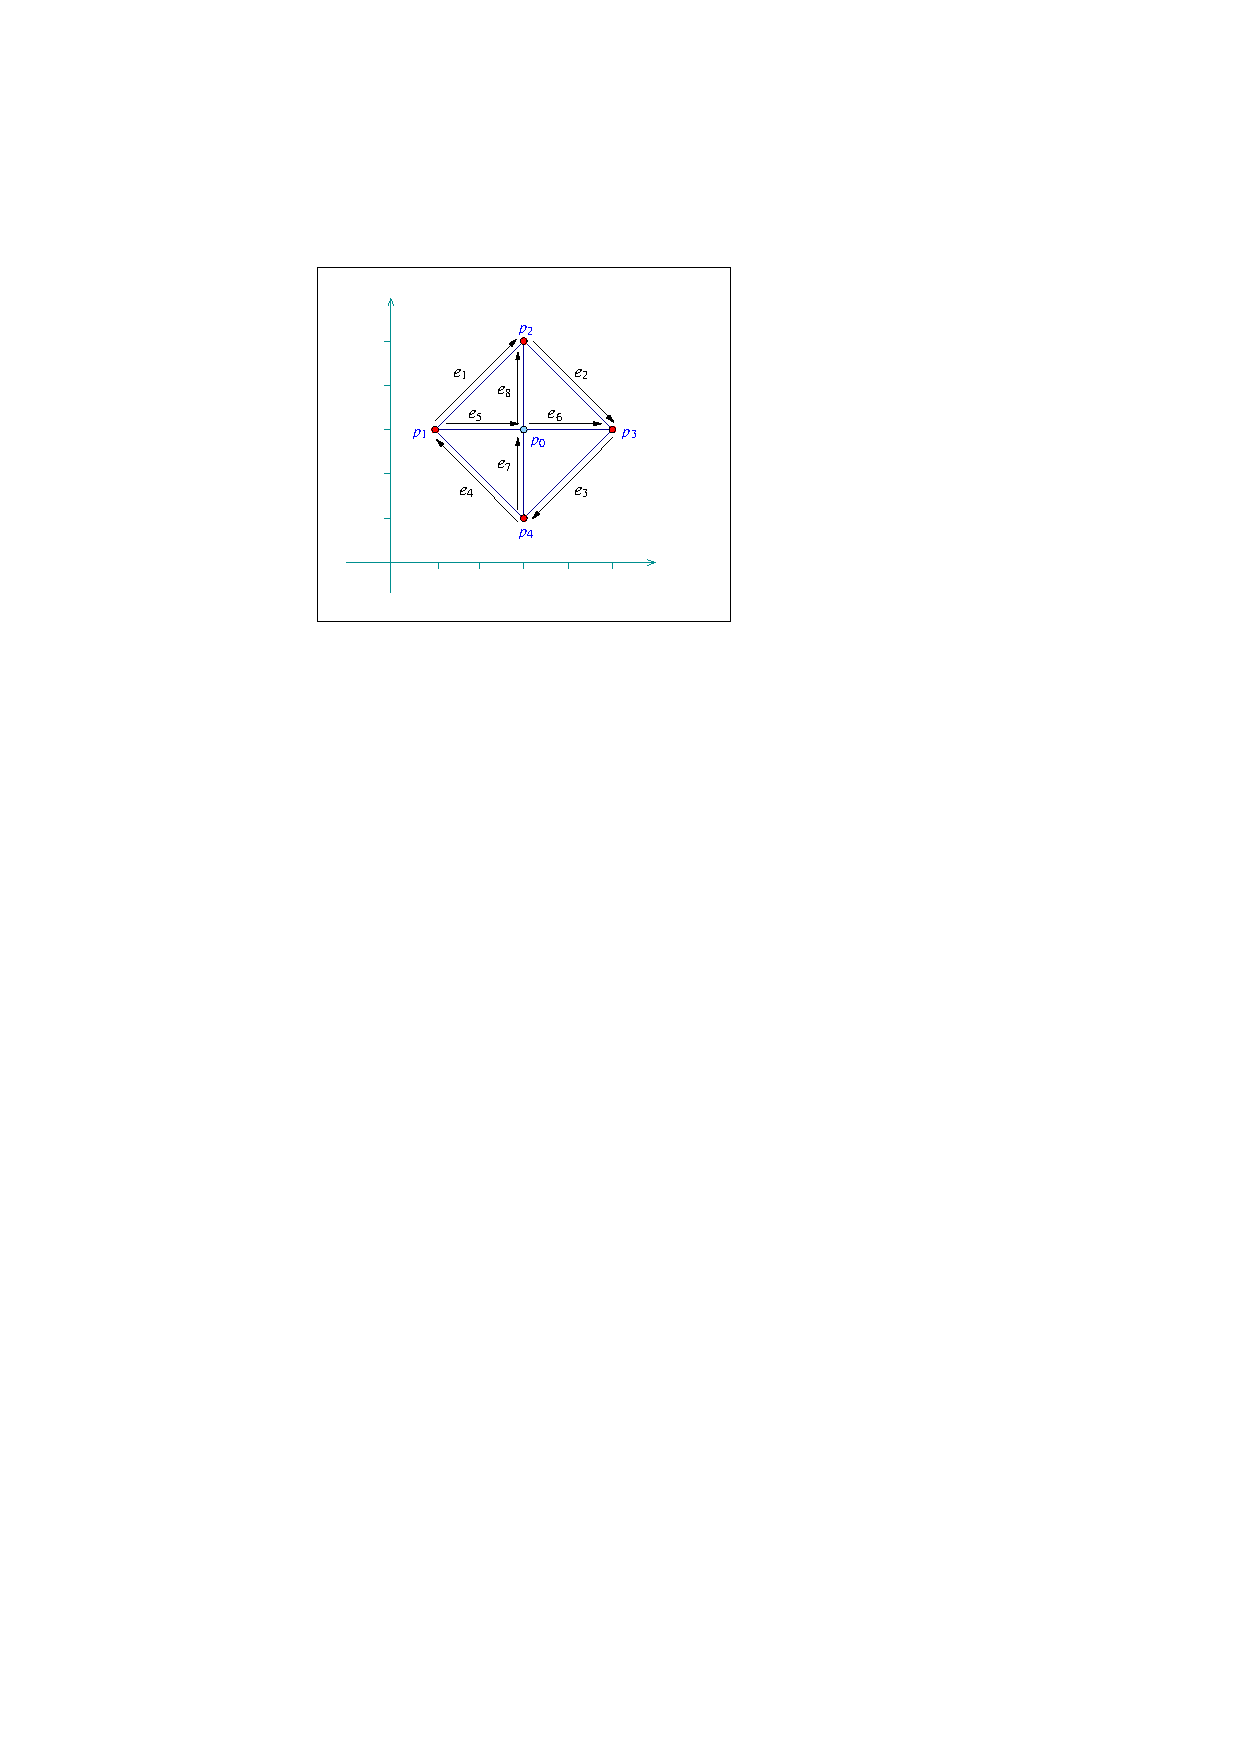
\includegraphics{Arrangement_2/fig/ex_4}
  \end{center}
\end{ccTexOnly}
\begin{ccHtmlOnly}
  <p><center>
  <img src="./fig/ex_4.gif" border=0 alt="Example 4">
  </center>
\end{ccHtmlOnly}
\caption{An arrangement of line segments, as constructed in
\ccc{ex_special_edge_insertion.C}. Note that $p_0$ is initially inserted as an
isolated point and later on connected to the other four
vertices.\label{arr_fig:ex_4}}
\end{figure}

The following program shows how to construct the arrangement
depicted in Figure~\ref{arr_fig:ex_4} using the specialized
insertion functions that accept predecessor halfedges:

\ccIncludeExampleCode{../examples/Arrangement_2/ex_special_edge_insertion.cpp}

It is possible to perform even more refined operations on an
\ccc{Arrangement_2} instance given specific topological information.
As most of these operations are very fragile and perform no precondition
testing on their input in order to gain efficiency, they are not included
in the public interface of the arrangement class. Instead, the
\ccc{Arr_accessor<Arrangement>} class allows access to these internal
arrangement operations --- see more details in the Reference Manual.
\end{ccAdvanced}

\section{Issuing Queries on an Arrangement\label{arr_sec:queries}}
%==========================================

One of the most important query types defined on arrangements is
the {\em point-location} query: Given a point, find the
arrangement cell that contains it. Typically, the result of a
point-location query is one of the arrangement faces, but in
degenerate situations the query point can be located on an edge or
coincide with a vertex.

Point-location queries are not only common in many applications,
they also play an important role in the free insertion-functions
(see Section~\ref{arr_sec:gl_funcs}). Therefore, it is crucial to
have the ability to answer such queries effectively for any
arrangement instance.

\subsection{Point-Location Queries\label{arr_ssec:pl}}
%----------------------------------

The arrangement package includes several classes (more precisely,
class templates parameterized by an arrangement class) that model
the \ccc{ArrangementPointLocation_2} concept. Namely, they all
have a member function called \ccc{locate(q)} that accepts a query
point $q$ and result with a \cgal\ \ccc{Object} that wraps a handle
to the arrangement cell containing the query point. This object can
be assigned to either a \ccc{Face_const_handle},
\ccc{Halfedge_const_handle} or a \ccc{Vertex_const_handle}, depending
on whether the query point is located inside a face, on an edge or
on a vertex.

Note that the handles returned by the \ccc{locate()} functions are
\ccc{const} (non-mutable) handles. If necessary, such handles may
be casted to mutable handles using the static functions
\ccc{Arrangement_2::non_const_handle()} provided by the
arrangement class.

An instance of any point-location class must be attached to an
\ccc{Arrangement_2} instance so we can use it to issue point-location
queries. This attachment can be performed when the point-location
instance is constructed, or at a later time, using the \ccc{init(arr)}
method, where \ccc{arr} is the attached \ccc{Arrangement_2} instance.
In this chapter we always use the first option.

The following function template, which can be found in the example
file \ccc{point_location_utils.h}, accepts a point-location object
(whose type can be any of the models to the
\ccc{ArrangementPointLocation_2} concept) and a query point, and
prints out the result of the point-location query for the given
point. Observe how we use the function \ccc{CGAL::assign()} is order
to cast the resulting \ccc{CGAL::Object} into a handle to an arrangement
feature. The point-location object \ccc{pl} is assumed to be already
associated with an arrangement:

\begin{alltt}
template <class PointLocation>
void point_location_query
        (const PointLocation& pl,
         const typename PointLocation::Arrangement_2::Point_2& q)
\{
  // Perform the point-location query.
  CGAL::Object obj = pl.locate (q);

  // Print the result.
  typedef typename PointLocation::Arrangement_2  Arrangement_2;

  typename Arrangement_2::Vertex_const_handle    v;
  typename Arrangement_2::Halfedge_const_handle  e;
  typename Arrangement_2::Face_const_handle      f;

  std::cout << "The point " << q << " is located ";
  if (CGAL::assign (f, obj)) \{
    // q is located inside a face:
    if (f->is_unbounded())
      std::cout << "inside the unbounded face." << std::endl;
    else
      std::cout << "inside a bounded face." << std::endl;
  \}
  else if (CGAL::assign (e, obj)) \{
    // q is located on an edge:
    std::cout << "on an edge: " << e->curve() << std::endl;
  \}
  else if (CGAL::assign (v, obj)) \{
    // q is located on a vertex:
    if (v->is_isolated())
      std::cout << "on an isolated vertex: " << v->point() << std::endl;
    else
      std::cout << "on a vertex: " << v->point() << std::endl;
  \}
  else \{
    CGAL_assertion_msg (false, "Invalid object.");
  \}
\}
\end{alltt}

\subsubsection{Choosing a Point-Location Strategy\label{arr_sssec:pl_strat}}
%~~~~~~~~~~~~~~~~~~~~~~~~~~~~~~~~~~~~~~~~~~~~~~~~~

Each of the various point-location classes employs a different
algorithm or {\em strategy}\footnote{We use the term {\em strategy}
following the design pattern taxonomy~\cite{cgal:ghjv-dpero-95}.}
for answering queries:
\begin{itemize}
\item \ccc{Arr_naive_point_location<Arrangement>} locates the query
point \naive ly, by exhaustively scanning all arrangement cells.
%
\item \ccc{Arr_walk_along_a_line_point_location<Arrangement>}
simulates a traversal, in reverse order, along an imaginary vertical
ray emanating
from the query point: It starts from the unbounded face of the
arrangement and moves downward toward the query point until
locating the arrangement cell containing it.
%
\item \ccc{Arr_landmarks_point_location<Arrangement,Generator>}
uses a set of ``landmark'' points whose location in the
arrangement is known. Given a query point, it uses a \kdtree\ to
find the nearest landmark and then traverses the straight line
segment connecting this landmark to the query point.

There are various ways to select the landmark set in the
arrangement, determined by the \ccc{Generator} template parameter.
By default, the generator
class \ccc{Arr_landmarks_vertices_generator} is used and the
arrangement vertices are the selected landmarks, but other
landmark generators, such as sampling random points or
choosing points on a grid, are also available; see the
Reference Manual for more details.
%
\item \ccc{Arr_trapezoid_ric_point_location<Arrangement>} implements
Mulmuley's point-location algorithm~\cite{m-fppa-90} (see
also~\cite[Chapter~6]{bkos-cgaa-00}). The
arrangement faces are decomposed into simpler cells of constant
complexity known as {\em pseudo-trapezoids} and a search-structure
(a directed acyclic graph) is constructed on top of these cells,
allowing to locate the pseudo-trapezoid (hence the arrangement
cell) containing a query point in expected logarithmic time.
\end{itemize}

The main advantage of the first two strategies is that they do not
require any extra data, so the respective classes just store a
pointer to an arrangement object and operate directly on it.
Attaching such point-location objects to an existing arrangement
has virtually no running-time cost at all, but the query time is
linear in the size of the arrangement (the performance of the
``walk'' strategy is much better in practice, but its worst-case
performance is linear). Using these strategies is therefore
recommended only when a relatively small number of point-location
queries are issued by the application, or when the arrangement is
constantly changing (i.e., changes in the arrangement structure
are more frequent than point-location queries).

On the other hand, the landmarks and the trapezoid RIC strategies
require auxiliary data structures on top of the arrangement, which
they need to construct once they are attached to an arrangement
object and need to keep up-to-date as this arrangement changes.
The data structures needed by both strategies can be constructed
in $O(N \log N)$ time (where $N$ is the overall number of edges in
the arrangement),
but the construction needed by the landmark algorithm is in
practice significantly faster. In addition, although both
resulting data structures are asymptotically linear in size, the
\kdtree\ that the landmark algorithm stores needs significantly
less memory. We note that Mulmuley's algorithm guarantees a
logarithmic query time, while the query time for the landmark
strategy is only logarithmic on average --- and we may have
scenarios where the query time can be linear. In practice however,
the query times of both strategies are competitive. For a detailed
experimental comparison, see \cite{cgal:hh-eplca-05}

The main drawback in the current implementation of the landmark
strategy, compared to the trapezoidal RIC strategy, is that while
the updating the auxiliary data structures
related to the trapezoidal decomposition is done very efficiently,
the \kdtree\ maintained by the landmark algorithm needs to be
frequently rebuilt as the arrangement changes. In addition, using
the landmark point-location class adds some extra requirement
from the traits class (that is, the traits class should be a model
of a refined concept \ccc{ArrangementLandmarkTraits_2}; see
Section~\ref{arr_sec:traits} for the details). However, most
built-in traits classes that come with the \cgal\ public release
support these extra operations.

It is therefore recommended to use the
\ccc{Arr_landmarks_point_location} class when the application
frequently issues point-location queries on an
arrangement that only seldom changes. If the arrangement is more
dynamic and is frequently going through changes, the
\ccc{Arr_trapezoid_ric_point_location} class should be the
selected point-location strategy.

\subsubsection{An Example\label{arr_sssec:pl_ex}}
%~~~~~~~~~~~~~~~~~~~~~~~~~

\begin{figure}[t]
\begin{ccTexOnly}
  \begin{center}
  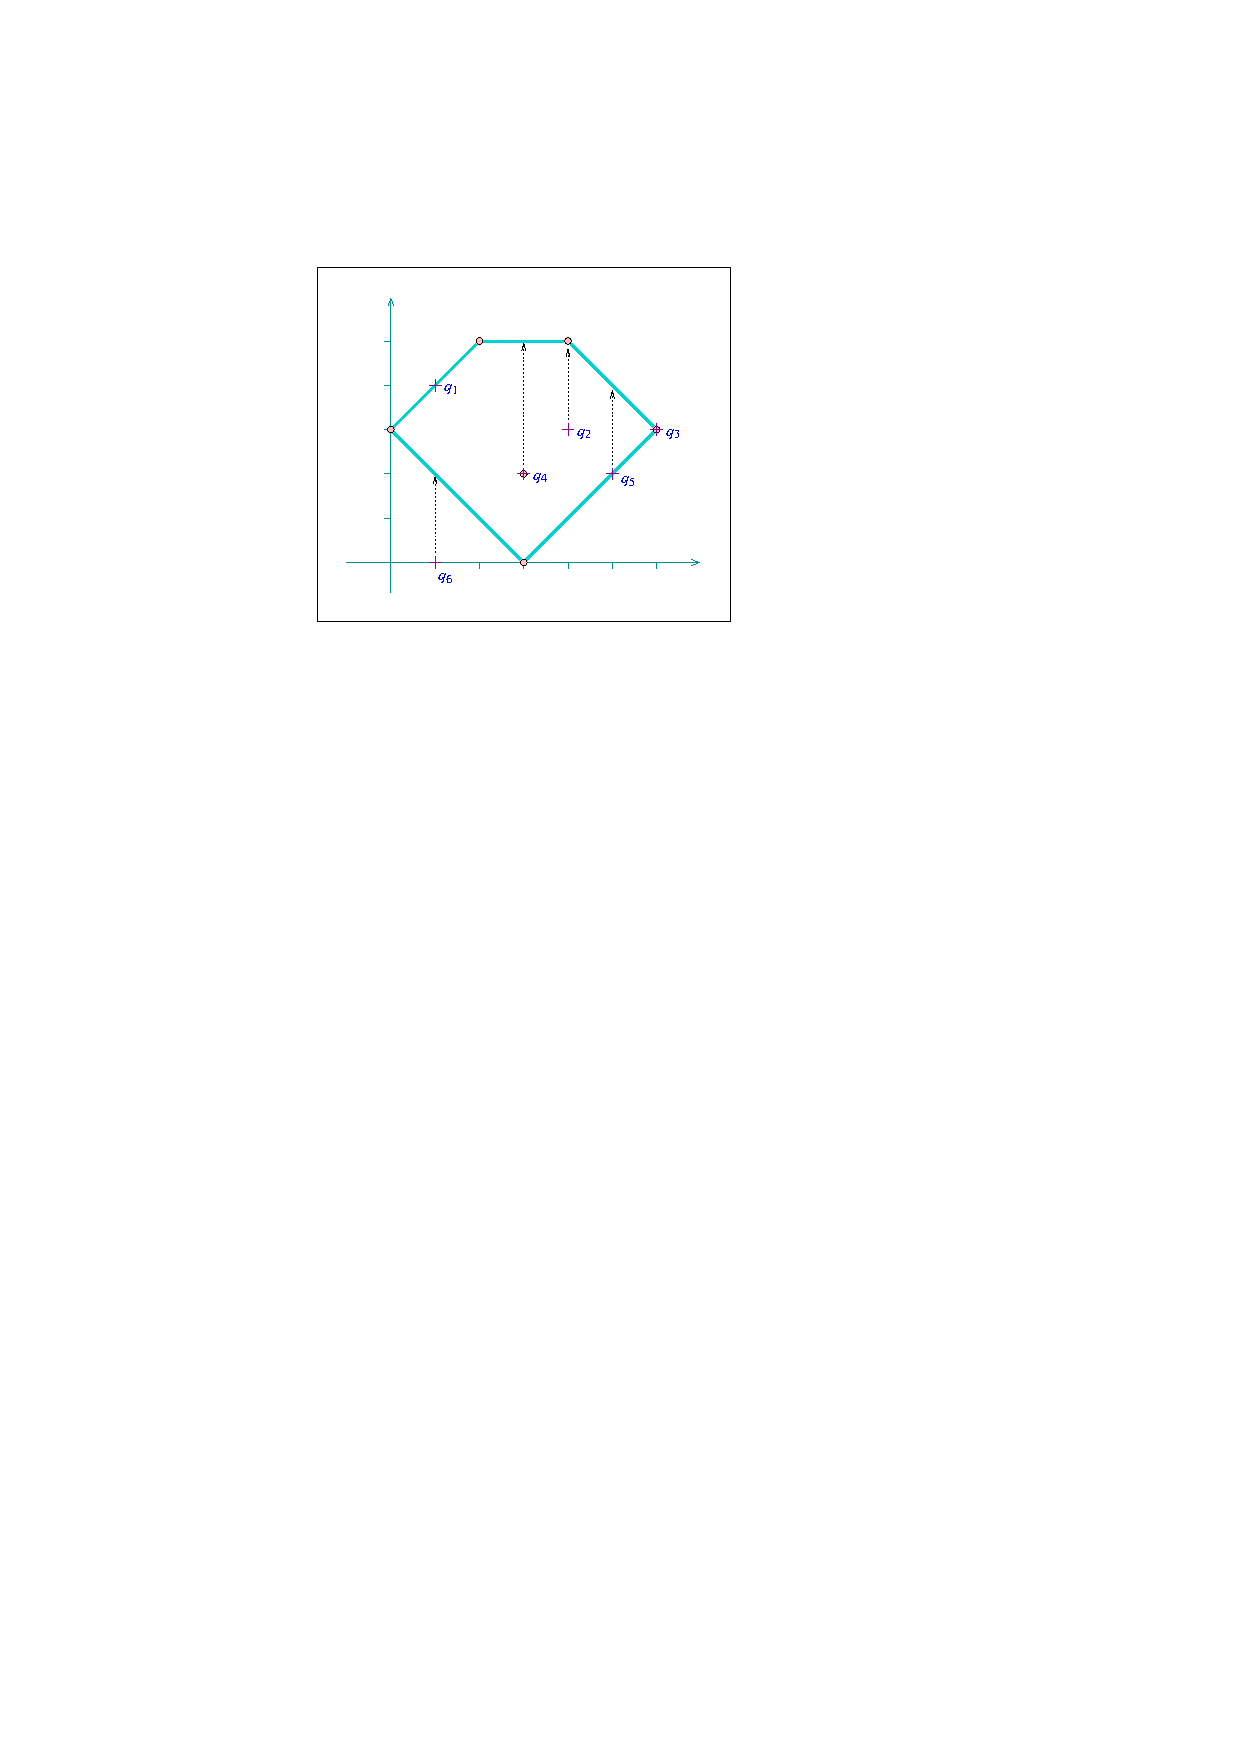
\includegraphics{Arrangement_2/fig/ex_5}
  \end{center}
\end{ccTexOnly}
\begin{ccHtmlOnly}
  <p><center>
  <img src="./fig/ex_5.gif" border=0 alt="Example 5">
  </center>
\end{ccHtmlOnly}
\caption{The arrangement of line segments, as constructed in
\ccc{point_location.cpp}, \ccc{vertical_ray_shooting.cpp}, and
\ccc{batched_point_location.cpp}. The
arrangement vertices are drawn as small discs, while the query
points $q_1, \ldots, q_6$ are marked with crosses.\label{arr_fig:ex_5}}
\end{figure}

The following program constructs a simple arrangement of five line
segments that form a pentagonal face, with a single isolated
vertex in its interior, as depicted in Figure~\ref{arr_fig:ex_5}
(the arrangement construction is performed by the function
\ccc{construct_segment_arr()} whose listing is omitted here and
can be found in \ccc{point_location_utils.h}).
It then employs the \naive\ and the landmark strategies to issue
several point-location queries on this arrangement:

\ccIncludeExampleCode{Arrangement_2/point_location.cpp}

Note that the program uses the auxiliary
\ccc{point_location_query()} function template to nicely print the
result of each query. This function can be found in the header file
\ccc{point_location_utils.h}.

\subsection{Vertical Ray Shooting\label{arr_ssec:ray_shoot}}
%---------------------------------

Another important query issued on arrangements is the vertical
ray-shooting query: Given a query point, which arrangement feature
do we encounter if we shoot a vertical ray emanating upward (or
downward) from this point? In the general case the ray hits an
edge, but it is possible that it hits a vertex, or that the
arrangement does not have any feature lying directly above (or
below) the query point.

All point-location classes listed in the previous section are also models
of the \ccc{ArrangementVerticalRayShoot_2} concept. That is, they all
have member functions called \ccc{ray_shoot_up(q)} and
\ccc{ray_shoot_down(q)} that accept a query point $q$ and output a
\cgal\ \ccc{Object}. This can be assigned to either a
\ccc{Halfedge_const_handle} or to a \ccc{Vertex_const_handle}.
Alternatively, the returned value is a \ccc{Face_const_handle}
for the unbounded face of the arrangement, in case there is no edge
or vertex lying directly above (or below) $q$.

The following function template, \ccc{vertical_ray_shooting_query()},
which also located in the header file \ccc{point_location_utils.h},
accepts a vertical ray-shooting
object, whose type can be any of the models to the
\ccc{ArrangementVerticalRayShoot_2} concept and prints out the
result of the upward vertical ray-shooting operations from a given
query point. The ray-shooting object \ccc{vrs} is assumed to be
already associated with an arrangement:

\begin{alltt}
template <class VerticalRayShoot>
void vertical_ray_shooting_query
    (const VerticalRayShoot& vrs,
     const typename VerticalRayShoot::Arrangement_2::Point_2& q)
\{
  // Perform the point-location query.
  CGAL::Object    obj = vrs.ray_shoot_up (q);

  // Print the result.
  typedef typename VerticalRayShoot::Arrangement_2  Arrangement_2;

  typename Arrangement_2::Vertex_const_handle    v;
  typename Arrangement_2::Halfedge_const_handle  e;
  typename Arrangement_2::Face_const_handle      f;

  std::cout << "Shooting up from " << q << " : "; 
  if (CGAL::assign (e, obj)) \{
    // We hit an edge:
    std::cout << "hit an edge: " << e->curve() << std::endl;
  \}
  else if (CGAL::assign (v, obj)) \{
    // We hit a vertex:
    if (v->is_isolated())
      std::cout << "hit an isolated vertex: " << v->point() << std::endl;
    else
      std::cout << "hit a vertex: " << v->point() << std::endl;
  \}
  else if (CGAL::assign (f, obj)) \{
    // We did not hit anything:
    CGAL_assertion (f->is_unbounded());
    
    std::cout << "hit nothing." << std::endl; 
  \}
  else \{
    CGAL_assertion_msg (false, "Invalid object.");
  \}
\}
\end{alltt}

The following program uses the auxiliary function listed above to
perform vertical ray-shooting queries on an arrangement.
The arrangement and the query points are exactly the same as in
\ccc{point_location.cpp} (see Figure~\ref{arr_fig:ex_5}):

\ccIncludeExampleCode{Arrangement_2/vertical_ray_shooting.cpp}

The number type we use in this example is \cgal's built-in
\ccc{MP_Float} type which is a floating-point number with an
unbounded mantissa and a 32-bit exponent. It supports construction from an
integer or from a machine \ccc{float} or \ccc{double} and performs additions,
subtractions and multiplications in an exact number.

\subsection{Batched Point-Location\label{arr_ssec:batched_pl}}
%----------------------------------

Suppose that at a given moment our application has to issue a
relatively large number $m$ of point-location queries on a
specific arrangement instance. It is possible of course to define
a point-location object and to issue separate queries on the
arrangement. However, as explained in Section~\ref{arr_ssec:pl},
choosing a simple point-location strategy (either the \naive\ or
the walk strategy) means inefficient queries, while the more
sophisticated strategies need to construct auxiliary structures
that incur considerable overhead in running time.

On the other hand, the arrangement package includes a free
\ccc{locate()} function that accepts an arrangement a range of
query points as its input and sweeps through the arrangement to
locate all query points in one pass. The function outputs the query
results as pairs, where each pair is comprised of a query point
and a \cgal\ \ccc{Object} that represents the cell containing the
point (see Section~\ref{arr_ssec:pl}). The output pairs are
sorted in increasing $xy$-lexicographical order of the query point.

The batched point-location operation can be performed in
$O\left((m+N)\log{(m+N)}\right)$ time, where $N$ is the number of
edges in the arrangement. This means that when the number $m$ of
point-location queries is of the same order of magnitude as $N$,
this operation is more efficient than issuing separate queries.
This suggestion is also backed up by experimental results.
Moreover, the batched point-location operation is also
advantageous as it does not have to construct and maintain
additional data structures.

The following program issues a batched point-location query, which
is essentially equivalent to the six separate queries performed in
\ccc{point_location.cpp} (see Section~\ref{arr_ssec:pl}):

\ccIncludeExampleCode{Arrangement_2/batched_point_location.cpp}

\section{Free Functions in the Arrangement Package\label{arr_sec:gl_funcs}}
%==================================================

In Section~\ref{arr_sec:arr_class} we reviewed in details the
\ccc{Arrangement_2} class, which represents two-dimensional
subdivisions induced by planar curves, and mentioned that its
interface is minimal in the sense that the member functions hardly
perform any geometric algorithms and are mainly used for
maintaining the topological structure of the subdivision. In this
section we explain how to utilize the free (global) functions that operate
on arrangements. The implementation of these operations typically require
non-trivial geometric algorithms or load some extra requirements on
the traits class.

\subsection{Incremental Insertion Functions\label{arr_ssec:inc_insert}}
%-------------------------------------------

\subsubsection{Inserting Non-Intersecting Curves\label{arr_sssec:insert_non_x}}
%~~~~~~~~~~~~~~~~~~~~~~~~~~~~~~~~~~~~~~~~~~~~~~~~

In Section~\ref{arr_sec:arr_class} we explained how to construct
arrangements of $x$-monotone curves that are pairwise disjoint in
their interior, when the location of the segment endpoints in the
arrangement is known. Here we relax this constraint, and allow the
location of the inserted $x$-monotone curve endpoints to be arbitrary,
as it may be unknown at the time of insertion. We retain, for the moment,
the requirement that the interior of the inserted curve is disjoint from
all existing arrangement edges and vertices.

The free function \ccc{insert_non_intersecting_curve(arr, c, pl)}
inserts the $x$-monotone curve $c$ into the arrangement \ccc{arr},
with the precondition that the interior of $c$ is disjoint from
all \ccc{arr}'s existing edges and vertices. The third argument
\ccc{pl} is a point-location object attached to the arrangement,
which is used for performing the insertion. It locates both curve
endpoints in the arrangement, where each endpoint is expected to
either coincide with an existing vertex or lie inside a face.
It is possible to invoke one of the specialized insertion functions
(see Section~\ref{arr_sec:arr_class}), based on the query results, and
insert $c$ at its proper position.\footnote{The
\ccc{insert_non_intersecting_curve()} function, as all other functions
reviewed in this section, is a function template, parameterized by an
arrangement class and a point-location class (a model of the
\ccc{ArrangementPointLocation_2} concept).} The insertion operation
thus hardly requires any geometric operations on top on the ones
needed to answer the point-location queries. Moreover, it is
sufficient that the arrangement class is instantiated with a
traits class that models the \ccc{ArrangementBasicTraits_2}
concept (or the \ccc{ArrangementLandmarkTraits_2} concept, if the
landmark point-location strategy is used), which does not have to
support the computation of intersection points between curves.

The variant \ccc{insert_non_intersecting_curve(arr, c)} is also
available. Instead of accepting a user-defined point-location
object, it defines a local instance of the walk point-location
class and uses it to insert the curve.

\subsubsection{Inserting $x$-Monotone Curves\label{arr_sssec:insert_x_mon}}
%~~~~~~~~~~~~~~~~~~~~~~~~~~~~~~~~~~~~~~~~~~~~

The \ccc{insert_non_intersecting_curve()} function is very
efficient, but its preconditions on the input curves are still
rather restricting. Let us assume that the arrangement is
instantiated with a traits class that models the refined
\ccc{ArrangementXMonotoneTraits_2} concept and supports
intersection computations (see Section~\ref{arr_sec:traits} for
the exact details). Given an $x$-monotone curve, it is sufficient
to locate its left endpoint in the arrangement and to trace its
{\em zone}, namely the set of arrangement features crossing the curve,
until the right endpoint is reached. Each time the new curve $c$
crosses an existing vertex or an edge, the curve is split into
subcurves (in the latter case, we have to split the curve 
associated with the existing halfedge as well) and associate new
edges with the resulting subcurves. Recall that an edge is represented
by a pair of twin halfedges, so we split it into two halfedge pairs.

The free function \ccc{insert_x_monotone_curve(arr, c, pl)} performs
this insertion operation. It accepts an $x$-monotone curve $c$,
which may intersect some of the curves already in the arrangement
\ccc{arr}, and inserts it into the arrangement by computing its zone.
Users may supply a point-location object \ccc{pl}, or use the default
walk point-location strategy (namely, the variant
\ccc{insert_x_monotone_curve(arr, c)} is also available). The
running-time of this insertion function is proportional to the
complexity of the zone of the curve $c$.

\begin{ccAdvanced}
In some cases users may have a prior knowledge of the location of the
left endpoint of the $x$-monotone curve \ccc{c} they wish to insert,
so they can perform the insertion without issuing any point-location
queries. This can be done by calling
\ccc{insert_x_monotone_curve(arr, c, obj)}, where \ccc{obj} is an
object represents the location of \ccc{c}'s left endpoint in the
arrangement --- namely it wraps a \ccc{Vertex_const_handle}, a
\ccc{Halfedge_const_handle} or a \ccc{Face_const_handle} (see
also Section~\ref{arr_ssec:pl}).
\end{ccAdvanced}

\subsubsection{Inserting General Curves\label{arr_sssec:insert_gen}}
%~~~~~~~~~~~~~~~~~~~~~~~~~~~~~~~~~~~~~~~

So far all our examples were of arrangements of line segments,
where the \ccc{Arrangement_2} template was instantiated with the
\ccc{Arr_segment_traits_2} class. In this case, the fact that
\ccc{insert_x_monotone_curve()} accepts an $x$-monotone curve does not
seem to be a restriction, as all line segments are $x$-monotone
(note that we consider vertical line segments to be {\em weakly}
$x$-monotone).

Suppose that we construct an arrangement of circles. A circle is
obviously not $x$-monotone, so we cannot use
\ccc{insert_x_monotone_curve()} in this case.\footnote{Note that a key
operation performed by \ccc{insert_x_monotone_curve()} is to locate the
left endpoint of the curve in the arrangement. A circle, however, does
not have any endpoints!} However, it is possible to subdivide each circle
into two $x$-monotone circular arcs (its upper half and its lower
half) and to insert each $x$-monotone arc separately.

The free function \ccc{insert_curve()} requires that the traits class
used by the arrangement \ccc{arr} to be a model of the concept
\ccc{ArrangementTraits_2}, which refines the
\ccc{ArrangementXMonotoneTraits_2} concept. It has to define an
additional \ccc{Curve_2} type (which may differ from the
\ccc{X_monotone_curve_2} type), and support the subdivision of curves
of this new type into $x$-monotone curves (see the exact details in
Section~\ref{arr_sec:traits}). The \ccc{insert_curve(arr, c, pl)}
function performs the insertion of the curve $c$, which does not need
to be $x$-monotone, into the arrangement by subdividing it into
$x$-monotone subcurves and inserting each one separately. Users
may supply a point-location object \ccc{pl}, or use the default
walk point-location strategy by calling \ccc{insert_curve(arr, c)}.

\subsubsection{Inserting Points\label{arr_sssec:insert_point}}
%~~~~~~~~~~~~~~~~~~~~~~~~~~~~~~~

The arrangement class enables us to insert a point as an isolated
vertex in a given face. The free function
\ccc{insert_point(arr, p, pl)} inserts a vertex into \ccc{arr} that
corresponds to the point \ccc{p} at an arbitrary location. It uses
the point-location object \ccc{pl} to locate the point in the
arrangement (by default, the walk point-location strategy is used),
and acts according to the result as follows:
\begin{itemize}
\item If \ccc{p} is located inside a face, it is inserted as an
isolated vertex inside this face.
\item If \ccc{p} lies on an edge, the edge is split to create a
vertex associated with \ccc{p}.
\item Otherwise, \ccc{p} coincides with an existing vertex and
we are done.
\end{itemize}
In all cases, the function returns a handle to the vertex
associated with \ccc{p}.

The arrangement \ccc{arr} should be instantiated with a traits class
that models the \ccc{ArrangementXMonotoneTraits_2} concept, as the
insertion operation may involve splitting curves.

\subsubsection{An Example\label{arr_sssec:insert_ex}}
%~~~~~~~~~~~~~~~~~~~~~~~~~~

\begin{figure}[t]
\begin{ccTexOnly}
  \begin{center}
  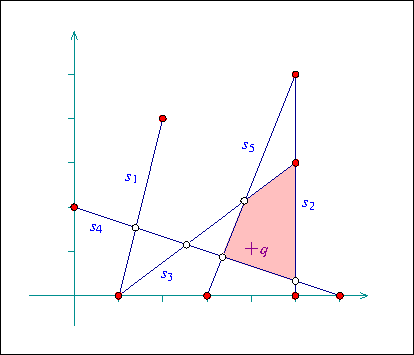
\includegraphics{Arrangement_2/fig/ex_8}
  \end{center}
\end{ccTexOnly}
\begin{ccHtmlOnly}
  <p><center>
  <img src="./fig/ex_8.gif" border=0 alt="Example 8">
  </center>
\end{ccHtmlOnly}
\caption{An arrangement of five intersecting line segments, as
constructed in \ccc{ex_incremental_insertion.cpp} and
\ccc{ex_aggregated_insertion.cpp}. The segment
endpoints are marked by black disks and the arrangement vertices
that correspond to intersection points are marked by circles.
The query point $q$ is marked with a cross and the face that
contains it is shaded.\label{arr_fig:ex_8}}
\end{figure}

The program below constructs an arrangement of intersecting
line-segments. We know that $s_1$ and $s_2$ do not intersect, so
we use \ccc{insert_non_intersecting_curve()} to insert them into the
empty arrangement. The rest of the segments are inserted using
\ccc{insert_x_monotone_curve()} or \ccc{insert_curve()}, which are
equivalent in case of line segments. The resulting arrangement consists
of $13$ vertices, $16$ edges, and $5$ faces, as can be seen in
Figure~\ref{arr_fig:ex_8}.

In the earlier examples, all arrangement vertices corresponded to
segment endpoints. In this example we have additional vertices that
correspond to intersection points between two segments. The
coordinates of these intersection points are rational numbers, if
the input coordinates are rational (or integer). Therefore,
the \ccc{Quotient<int>} number type is used to represent the
coordinates:

\ccIncludeExampleCode{Arrangement_2/ex_incremental_insertion.cpp}

\subsection{Aggregated Insertion Functions\label{arr_ssec:agg_insert}}
%------------------------------------------

Let us assume that we have to insert a set of $m$ input curves into an
arrangement. It is possible to do this incrementally, 
inserting the curves one by one, as shown in the previous section.
However, the arrangement package provides three free functions that
aggregately insert a range of curves into an arrangement:
%
\begin{itemize}
\item \ccc{insert_non_intersecting_curves(arr, begin, end)} inserts 
a range of $x$-monotone curves given by the input iterators
\ccc{[begin, end)} into an arrangement \ccc{arr}. The $x$-monotone
curves should be pairwise disjoint in their interior and also
interior-disjoint from all existing edges and vertices of \ccc{arr}.
%
\item \ccc{insert_x_monotone_curves(arr, begin, end)} operates on
a range of $x$-monotone curves that may intersect one another.
%
\item \ccc{insert_curves(arr, begin, end)} inserts a range of
of general (not necessarily $x$-monotone) curves of type \ccc{Curve_2},
given by the input iterators \ccc{[begin, end)}, into the arrangement
\ccc{arr}.
\end{itemize}

We distinguish between two cases: (i) The given arrangement
\ccc{arr} is empty (has only an unbounded face), so we have to
construct it from scratch. (ii) We have to insert $m$ input curves
to a non-empty arrangement \ccc{arr}.

In the first case, we sweep over the input curves, compute
their intersection points and construct the \dcel\ that represents
their planar arrangement. This process is performed in
$O\left((m + k)\log m\right)$ time, where $k$ is the total number
of intersection points. The running time is asymptotically better
than the time needed for incremental insertion, if the arrangement
is relatively sparse (when $k$ is bounded by $\frac{m^2}{\log
m}$), but in practice it is recommended to use this aggregated
construction process even for dense arrangements, since the
sweep-line algorithm needs less geometric operations compared to
the incremental insertion algorithms and hence typically runs 
much faster in practice.

Another important advantage the aggregated insertion functions
have is that they do not issue point-location queries. Thus, no
point-location object needs to be attached to the arrangement. As
explained in Section~\ref{arr_ssec:pl}, there is a trade-off
between construction time and query time in each of the
point-location strategies, which affects the running times of the
incremental insertion process. Naturally, this trade-off is irrelevant
in case of aggregated insertion as above.

The example below shows how to construct the arrangement of
line segments depicted in Figure~\ref{arr_fig:ex_8} and built
incrementally in \ccc{ex_incremental_insertion.cpp}, as shown in the previous
section. We use the aggregated insertion function
\ccc{insert_x_monotone_curves()} as we deal with line segments.
Note that no point-location object needs to be defined and attached to the
arrangement:

\ccIncludeExampleCode{Arrangement_2/ex_aggregated_insertion.cpp}

In case we have to insert a set of $m$ curves into an existing
arrangement, where we denote the number of edges in the arrangement by $N$.
As a rule of thumb, if $m = o(\sqrt{N})$, we insert the curves one by
one. For larger input sets, we use the aggregated insertion procedures.

\begin{figure}[t]
\begin{ccTexOnly}
  \begin{center}
  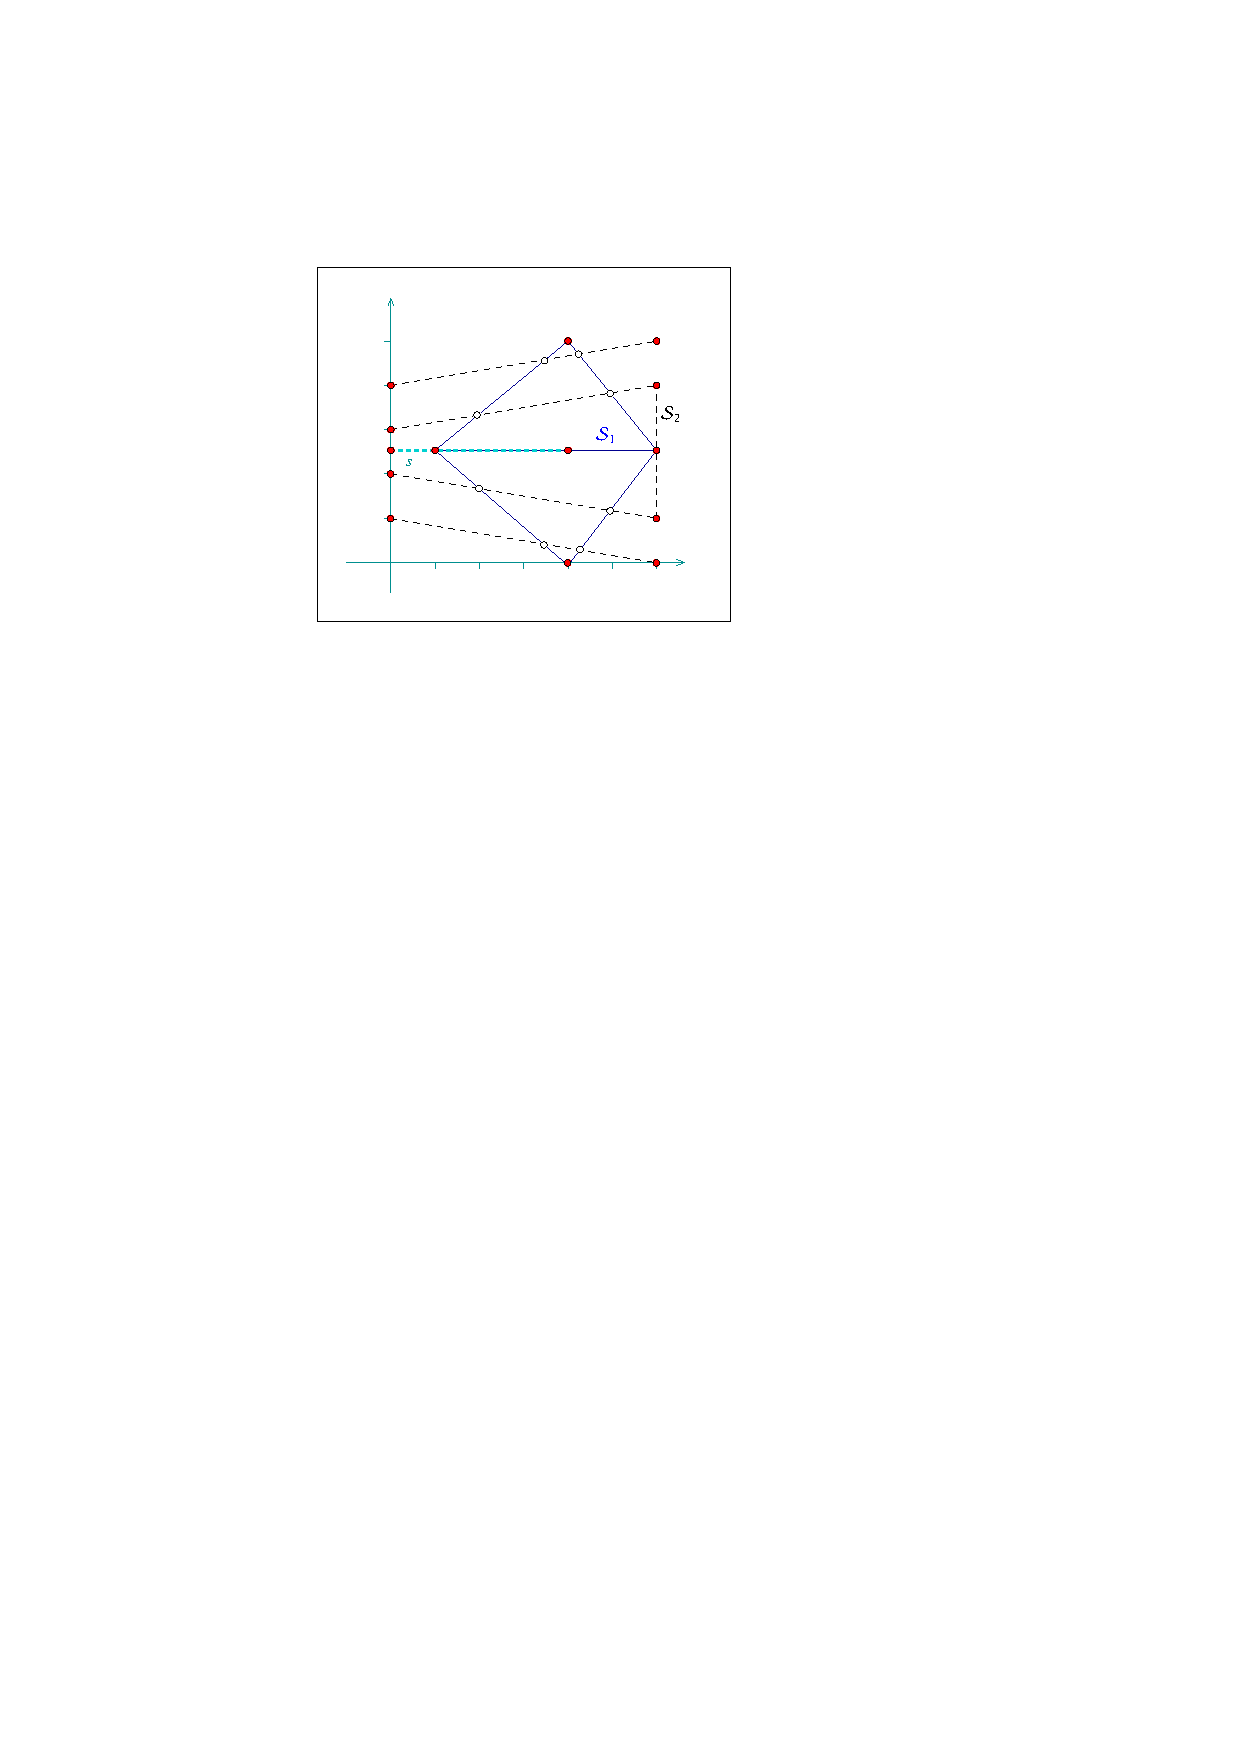
\includegraphics{Arrangement_2/fig/ex_10}
  \end{center}
\end{ccTexOnly}
\begin{ccHtmlOnly}
  <p><center>
  <img src="./fig/ex_10.gif" border=0 alt="Example 10">
  </center>
\end{ccHtmlOnly}
\caption{An arrangement of intersecting line segments, as
constructed in \ccc{ex_global_insertion.cpp}. The segments of ${\mathcal S}_1$
are drawn in solid lines and the segments of ${\mathcal S}_2$ are
drawn in dark dashed lines. Note that the segment $s$ (light
dashed line) overlaps one of the segments in
${\mathcal S}_1$.\label{arr_fig:ex_10}}
\end{figure}

In the example below we aggregately construct an arrangement of a set
${\mathcal S}_1$ containing five line segments. Then we insert a single
segment using the incremental insertion function. Finally, we add a set
${\mathcal S}_2$ with five more line segments in an aggregated fashion.
Notice that the line segments of ${\mathcal S}_1$ are pairwise
interior-disjoint, so we use \ccc{insert_non_intersecting_curves()}.
${\mathcal S}_2$ also contain pairwise interior-disjoint segments,
but as they intersect the existing arrangement, we have to use
\ccc{insert_x_monotone_curves()} to insert them. Also note that the
single segment $s$ we insert incrementally overlaps an existing
arrangement edge:

\ccIncludeExampleCode{Arrangement_2/ex_global_insertion.cpp}

The number type used in the example above,
\ccc{Quotient<MP_Float>}, is comprised of a numerator and a
denominator of type \ccc{MP_Float}, namely floating-point numbers
with unbounded mantissa. This number type is therefore capable of
exactly computing the intersection points as long as the segment
endpoints are given as floating-point numbers.

\subsection{Removing Vertices and Edges\label{arr_ssec:gl_remove}}
%---------------------------------------

The free functions \ccc{remove_vertex()} and \ccc{remove_edge()} handle
the removal of vertices and edges from an arrangement. The difference
between these functions and the member functions of the \ccc{Arrangement_2}
template having the same name is that they allow the merger of two curves
associated with adjacent edges to form a single edge. Thus, they require
that the traits class that instantiates the arrangement instance is a model
of the refined \ccc{ArrangementXMonotoneTraits_2} concept (see
Section~\ref{arr_sec:traits}).

The function \ccc{remove_vertex(arr, v)} removes the vertex
\ccc{v} from the given arrangement \ccc{arr}, where \ccc{v} is
either an isolated vertex or is a {\em redundant} vertex ---
namely, it has exactly two incident edges that are associated with
two curves that can be merged to form a single $x$-monotone curve.
If neither of the two cases apply, the function returns an
indication that it has failed to remove the vertex.

The function \ccc{remove_edge(arr, e)} removes the edge \ccc{e}
from the arrangement by simply calling \ccc{arr.remove_edge(e)}
(see Section~\ref{arr_ssec:modify}). In addition, if either of the
end vertices of \ccc{e} becomes isolated or redundant after the removal
of the edge, it is removed as well.

\lcTex{%
  \setlength{\ArrangementTwoWidthRight}{1.5cm}
  \setlength{\ArrangementTwoWidthLeft}{\ArrangementTwoWidthLineReal}
  \addtolength{\ArrangementTwoWidthLeft}{-\ArrangementTwoWidthRight}
  \begin{minipage}{\ArrangementTwoWidthLeft}
}
\begin{ccHtmlOnly}
  <p><center>
    <img src="./fig/h_shape.gif" border=0 alt="h_shape" align=right>
  </center>
\end{ccHtmlOnly}
The following example demonstrates the usage of the free removal
functions. In creates an arrangement of four line segment forming
an H-shape with a double horizontal line. Then it removes the two
horizontal edges and clears all redundant vertices, such that the
final arrangement consists of just two edges associated with the
vertical line segments:
\lcTex{%
  \end{minipage}\hspace{\ArrangementTwoMinipageSpace}
  \begin{minipage}{\ArrangementTwoWidthRight}
    \begin{center}
    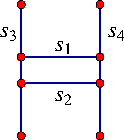
\includegraphics{Arrangement_2/fig/h_shape}
    \end{center}
  \end{minipage}
}

\ccIncludeExampleCode{Arrangement_2/ex_global_removal.cpp}

\section{Arrangements of Unbounded Curves\label{arr_sec:unbounded}}
%========================================

Previous sections dealt only with arrangements of line segments,
namely of bounded curves. Such arrangements always have one unbounded
face that contains all other arrangement features. This section
explains how to construct arrangements of unbounded curves, such as
lines and rays.

\subsection{Basic Manipulation and Traversal Methods\label{arr_ssec:unb_basic}}
%--------------------------------------------

Consider the arrangement induced by the two lines $y = x$ and
$y = -x$. These two line intersect at the origin, such that the
arrangement contains a single vertex $v = (0,0)$, with four infinite
rays emanating from it. Each ray corresponds to an arrangement edge,
and these edges subdivide the plane into four unbounded faces.
Consider a halfedge pair that represents one of the edges. The source
vertex of one of these halfedges is $v$ and its target is at infinity,
while the other has its source at infinity and $v$ is its target.

If \ccc{e} is an object of the nested type
\ccc{Arrangement_2::Halfedge}, then the predicates
\ccc{e.source_at_infinity()} and \ccc{e.target_at_infinity()} indicate
whether the halfedge represents a curve with an infinite end.
In general there is no need to access the source (or the target) of a
halfedge if it lies at infinity, since this vertex is not associated
with any valid point. Similarly, calling \ccc{arr.number_of_vertices()}
for an arrangement object \ccc{arr} counts only the vertices
associated with finite points, and ignores vertices at infinity
(and the range \ccc{[vertices_begin(), vertices_end())} contains only
finite vertices). The method \ccc{arr.number_of_vertices_at_infinity()}
counts the number of vertices at infinity.

As mentioned above, arrangements of unbounded curves usually have more
than one unbounded face. The function \ccc{arr.number_of_unbounded_faces()}
returns the number of unbounded arrangement faces
(Thus, \ccc{arr.number_of_faces() - arr.number_of_unbounded_faces()}
is the number of bounded faces).
The functions \ccc{arr.unbounded_faces_begin()} and
\ccc{arr.unbounded_faces_end()} return iterators of type
\ccc{Arrangement_2::Unbounded_face_iterator} that specify the range
of unbounded faces. Naturally, the value-type of this iterator is
\ccc{Arrangement_2::Face}.

The specialized insertion functions listed in
Section~\ref{arr_sssec:mf_insert_cv} can also be used for inserting
$x$-monotone unbounded curves, provided that they are interior-disjoint
from any subcurve that already exists in the arrangement. For example,
if you wish to insert a ray $r$ emanating from $(0,0)$ in the direction
of $(1,0)$, to the arrangement of $y = -x$ and $y = x$, you can use
the function \ccc{arr.insert_from_left_vertex()}, as the left
endpoint of $r$ is already associated with an arrangement vertex.
Other edge-manipulation functions can also be applied on edges
associated with unbounded curves.

\begin{figure}[t]
\begin{ccTexOnly}
  \begin{center}
  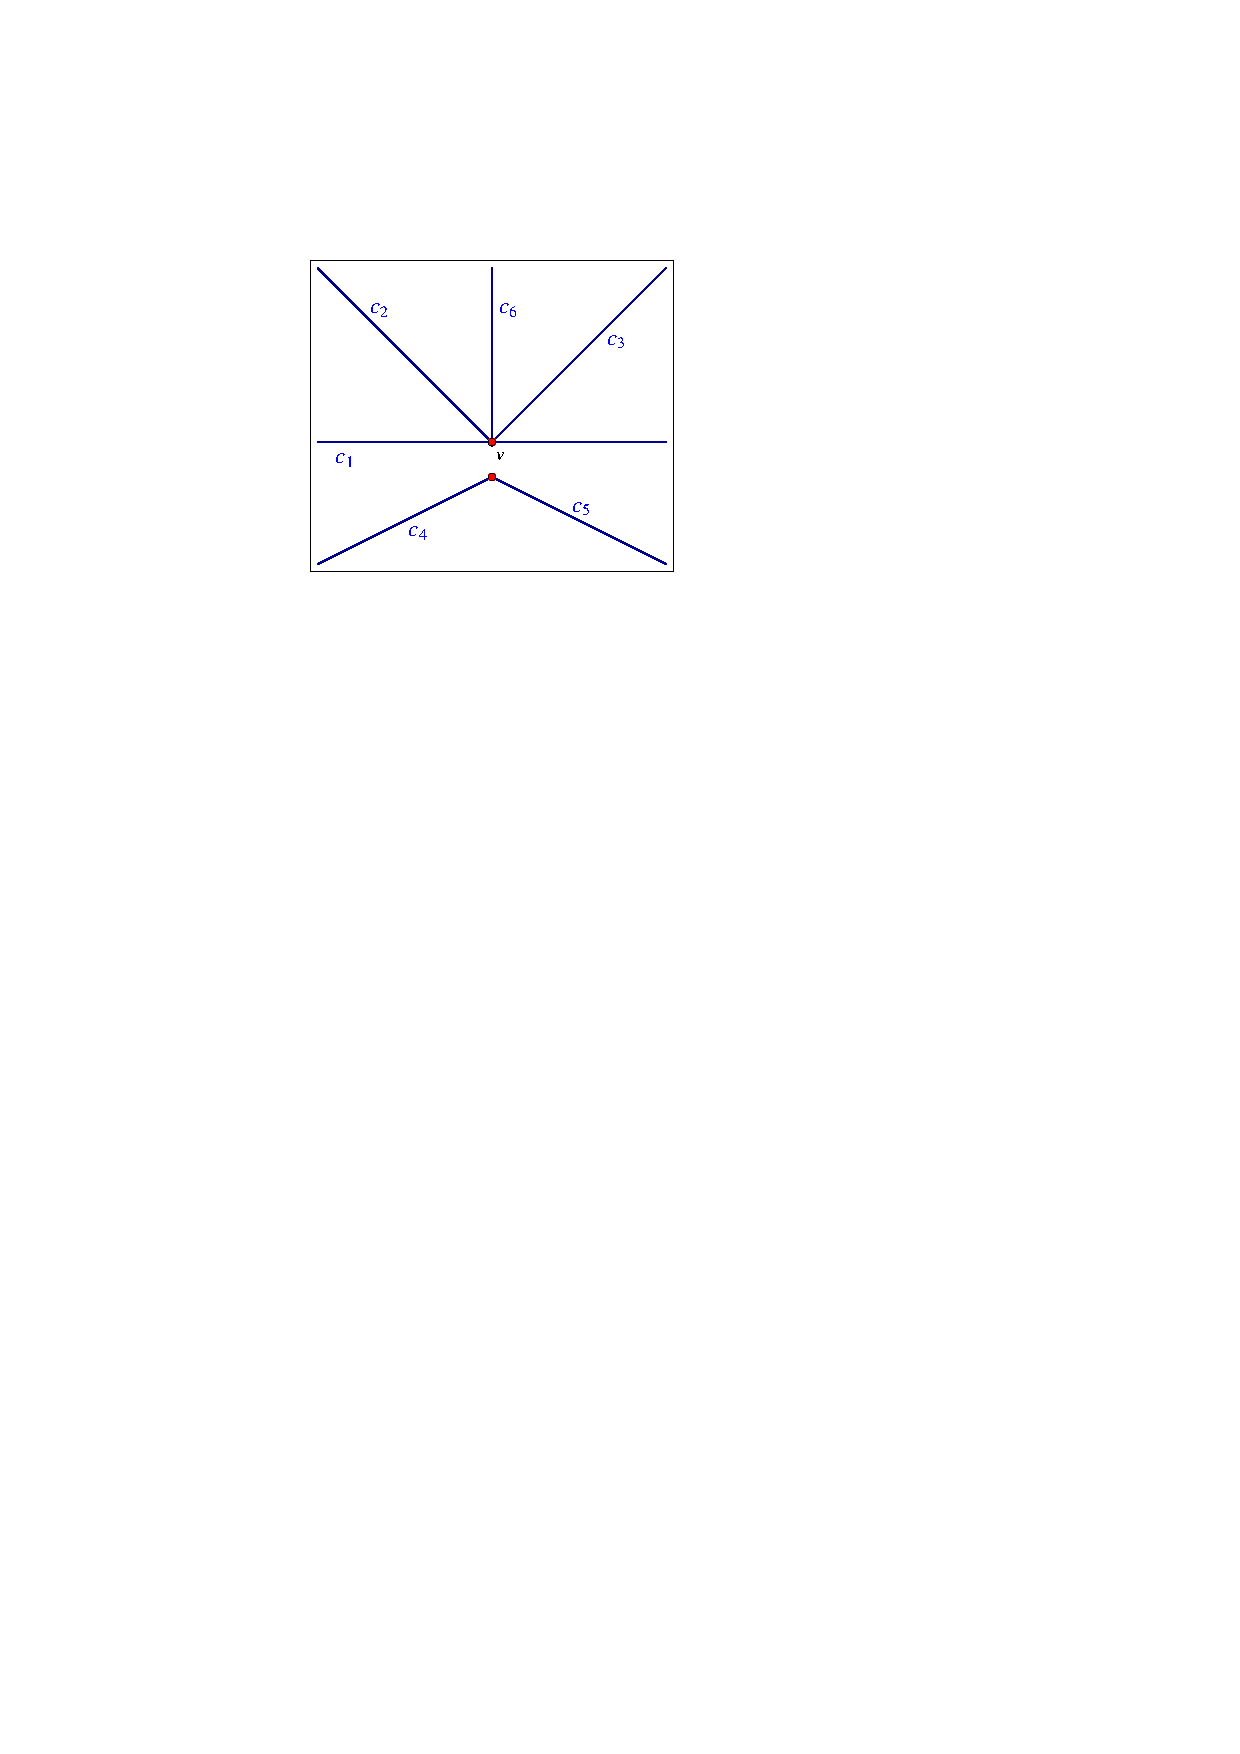
\includegraphics{Arrangement_2/fig/ex_unb1}
  \end{center}
\end{ccTexOnly}
\begin{ccHtmlOnly}
  <p><center>
  <img src="./fig/ex_unb1.gif" border=0 alt="Unbounded example 1">
  </center>
\end{ccHtmlOnly}
\caption{An arrangement of unbounded linear objects, as constructed
in \ccc{unbounded_non_intersecting.cpp}.\label{arr_fig:ex_unb1}}
\end{figure}

The following example demonstrates the use of the insertion function
for pairwise interior-disjoint unbounded curves. In this example
we use the traits class \ccc{Arr_linear_traits_2<Kernel>} to
instantiate the \ccc{Arrangement_2} template. This traits class is
capable of representing line segments as well as unbounded linear
curves (namely lines and rays). Observe that objects of the type
\ccc{X_monotone_curve_2} defined by this traits class are
constructible from \ccc{Line_2}, \ccc{Ray_2}, and \ccc{Segment_2}
objects, as defined in the instantiated kernel.

The first three curves are inserted using the special insertion
functions for $x$-monotone curves whose location in the arrangement
is known. Notice that inserting an unbounded curve in the interior
of an unbounded face, or from an existing vertex that represents the
bounded end of the curve, may cause an unbounded face to split (this
is never the case when inserting a bounded curve --- compare with
Section~\ref{arr_sssec:mf_insert_cv}). Then, three additional rays are 
inserted incrementally, using the insertion function for $x$-monotone
curves whose interior is disjoint from all arrangement features.
Finally, the program prints the size of the arrangement (compare to
the the illustration in Figure~\ref{arr_fig:ex_unb1}) and the outer
boundaries of its six unbounded faces:

\ccIncludeExampleCode{Arrangement_2/unbounded_non_intersecting.cpp}

\subsection{Free Functions\label{arr_ssec:unb_global}}
%---------------------------

In principle, all queries and operations that relate to arrangements
of bounded curves can also be applied to arrangements of unbounded
curves. For example, it is possible to issue point-location and
vertical ray-shooting queries (see also Section~\ref{arr_sec:queries})
on arrangements of lines, where the only restriction is that the query
point has finite coordinates.\footnote{Currently, all point-location
strategies except the trapezoidal RIC point-location strategy are
capable of handling arrangements of unbounded curves.} 

In the following example we show how an arrangement of unbounded lines
is utilized to solve the following problem: Given a set of points, does
the set contain at least three collinear points? In this example a set
of input points is read from a file. The file  \ccc{points.dat} is
used by default. It contains definitions of $100$ points randomly
selected on the grid $[-10000,10000]\times[-10000,10000]$. We
construct an arrangement of the dual lines, where the line $p^{*}$
dual to the point $p = (p_x, p_y)$ is given by the equation
$y = p_x*x - p_y$, and check whether three (or more) of the dual lines
intersect at a common point, by searching for a (dual) vertex, whose
degree is greater than $4$. If such a vertex exists, then there are at
least three dual lines that intersect at a common point, which implies
that there are at least three collinear points.

\ccIncludeExampleCode{Arrangement_2/dual_lines.cpp}

Note that there are no three collinear points among the points defined
in the input file \ccc{points.dat}. In the second part of the example
the existence of collinearity is forced and verified as follows. A line
dual to the midpoint of two randomly selected points is introduced,
and inserted into the arrangement. This operation is followed by a
test that verifies that a vertex of degree greater than $4$
exists. This implied that collinearity indeed exists as explained above.

\begin{ccAdvanced}

\subsection{Representation of Unbounded Arrangements\label{arr_ssec:unb_rep}}
%--------------------------------------------

\begin{figure}[t]
\begin{ccTexOnly}
  \begin{center}
  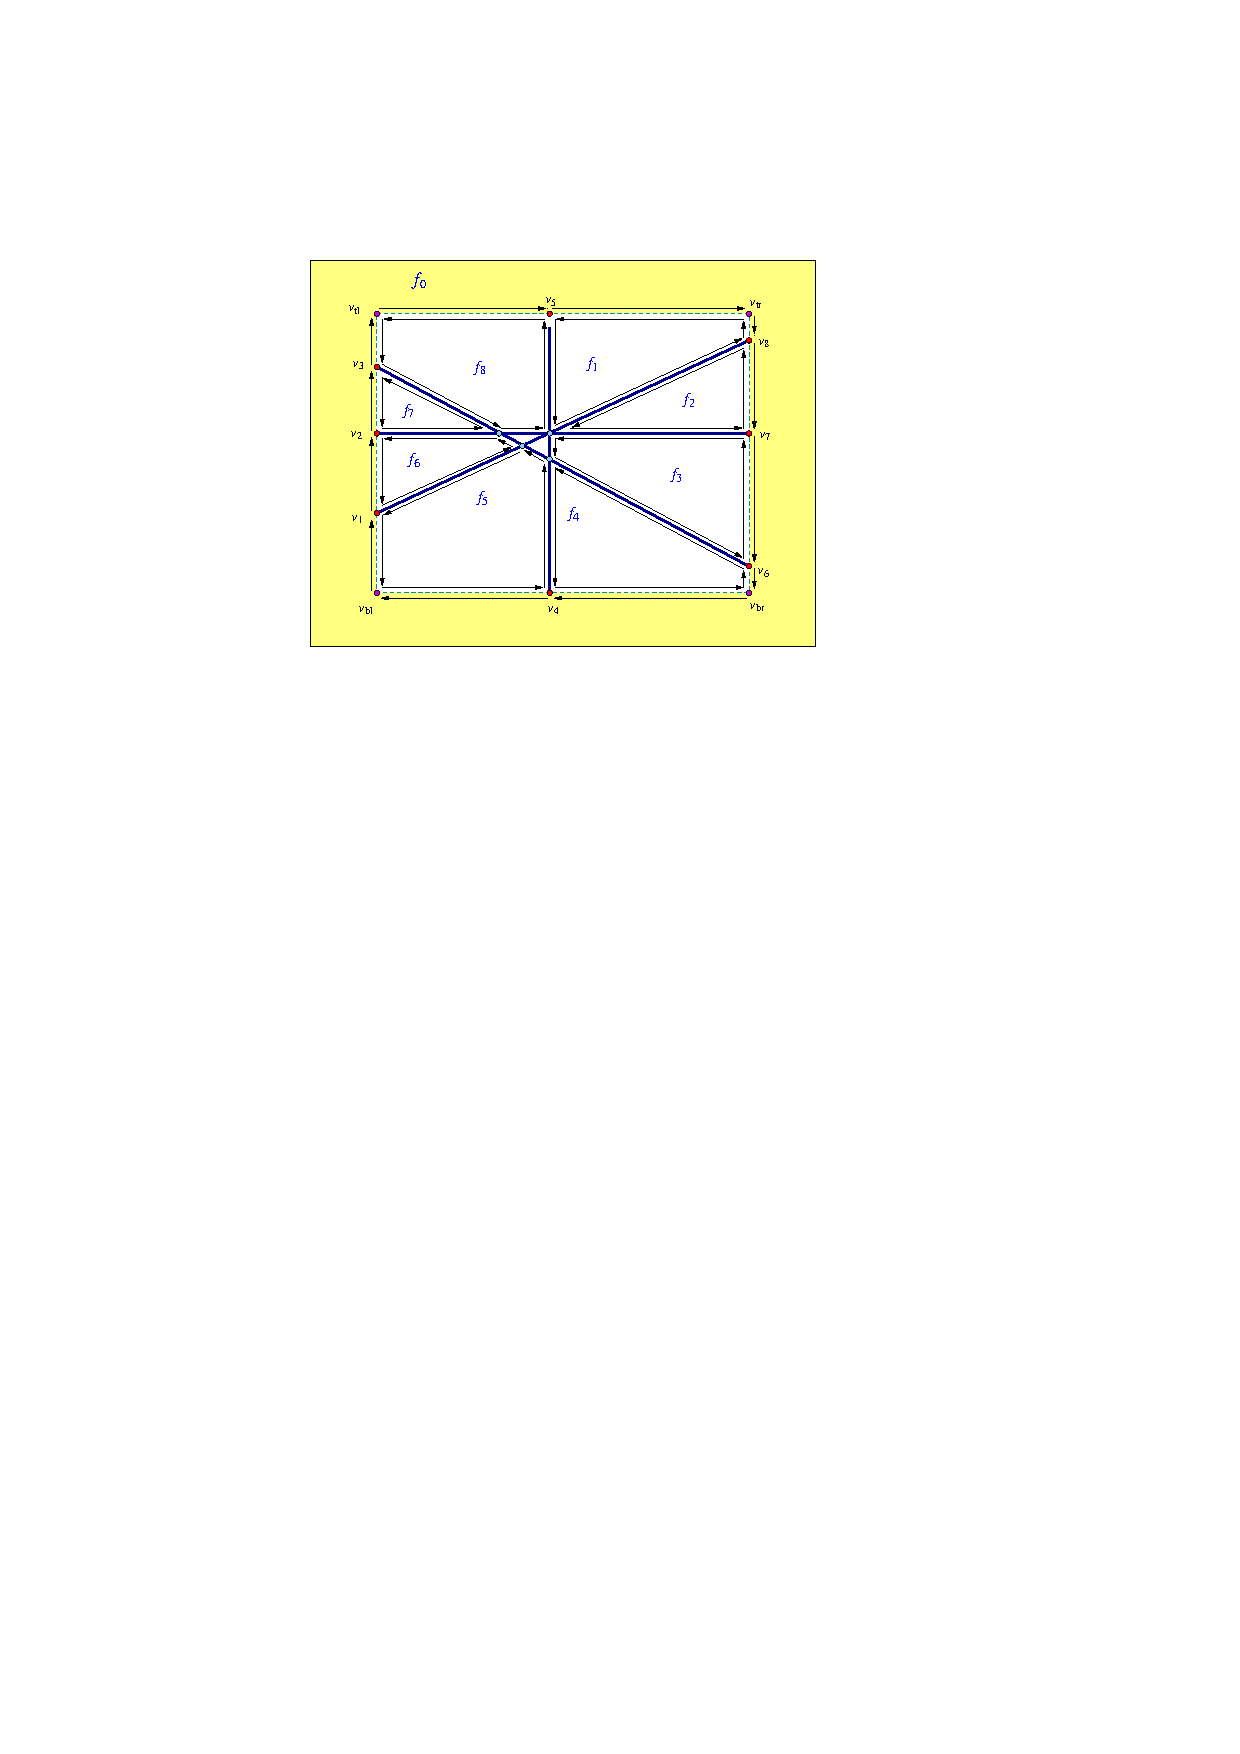
\includegraphics{Arrangement_2/fig/unb_dcel}
  \end{center}
\end{ccTexOnly}
\begin{ccHtmlOnly}
  <p><center>
  <img src="./fig/unb_dcel.gif" border=0 alt="Unbounded DCEL">
  </center>
\end{ccHtmlOnly}
\caption{A \dcel\ representing an arrangement of four lines.
Halfedges are drawn as thin arrows. The vertices $v_1, \ldots, v_8$
lie at infinity, and are not associated with valid points. The
halfedges that connect them are fictitious, and are not associated
with concrete curves. The face denoted $f_0$ (lightly shaded)
is the fictitious ``unbounded face'' which lies outside the imaginary
rectangle (dashed) that bounds the actual arrangement. The four
fictitious vertices $v_{\rm bl}, v_{\rm tl}, v_{\rm br}$ and
$v_{\rm tr}$ represent the four corners of the imaginary bounding
rectangle..\label{arr_fig:unb_dcel}}
\end{figure}

Given a set $\calC$ of unbounded curves, a simple approach for
representing the arrangement induced by $\calC$ would be to clip the
unbounded curves using an axis-parallel rectangle that contains all
finite curve endpoints and intersection points between curves in
$\calC$. This process would result in a set $\calC$ of bounded curves
(line segments if $\calC$ contains lines and rays), and it would be
straightforward to compute the arrangement induced by this set.
However, we would like to operate directly on the unbounded curves
without having to preprocess them. Therefore, we use an implicit
bounding rectangle embedded in the \dcel\ structure.
Figure~\ref{arr_fig:unb_dcel} shows the arrangement of four lines
that subdivide the plane into eight unbounded faces and two bounded
ones. Notice that in this case the unbounded faces have outer
boundaries, and the halfedges along these outer CCBs are drawn as 
arrows. The bounding rectangle is drawn with a dashed line. The
vertices $v_1,v_2,\ldots,v_8$, which represent the unbounded ends of 
the four lines, and lie on the bounding rectangle, actually exist at
infinity, and the halfedges connecting them are \emph{fictitious}, and
represent portions of the bounding rectangle. Note that the outer CCBs
of the unbounded faces contain fictitious halfedges. The twins of these
halfedges form together one connected component that corresponds to
the entire imaginary rectangle, which forms a single hole in a face
$\tilde{f}$. We say that $\tilde{f}$ is \emph{fictitious}, as it does
not corresponds to a real two-dimensional cell of the arrangement.

Observe that there are four extra vertices at infinity that do not lie
on any curve; they are denoted as $v_{\rm bl}, v_{\rm tl}, 
v_{\rm br}$, and $v_{\rm tr}$, and represent the bottom-left, top-left,
bottom-right, and top-right corners of the bounding rectangle,
respectively. Similarly, there are fictitious halfedges that lie on
the top, the bottom, the left, or the right edge of the imaginary
bounding rectangle. When the arrangement is empty, there are exactly
four pairs of fictitious halfedges, that divide the plane into two
faces, namely a fictitious face lying outside of the imaginary bounding
rectangle and a single unbounded face bounded by the imaginary
bounding rectangle. 

Summarizing the above, there are four types of arrangement vertices,
which differ from one another by their location on the imaginary
bounding rectangle:
\begin{enumerate}
\item
A ``normal'' vertex, associated with a point in $\real^2$ whose
coordinates are bounded. Such a vertex always lies inside the
bounding rectangle.
\item
A vertex that represent an unbounded end of an $x$-monotone curve
that is defined at $x = -\infty$ or at $x = \infty$. In case of
a horizontal line or a curve with a horizontal asymptote, the
$y$-coordinate of the curve end may be finite (see for example the
vertices $v_2$ and $v_7$ in Figure~\ref{arr_fig:unb_dcel}), but in
general the curve end also goes to $y = \pm\infty$ (see for instance
the vertices $v_1$, $v_3$, $v_6$ and $v_8$ in
Figure~\ref{arr_fig:unb_dcel}). For our convenience, we will always
take a ``tall'' enough bounding rectangle and treat such vertices as
lying on either the left or right rectangle edges (that is, if a curve
is defined at $x = -\infty$, its left end will be represented by
a vertex on the left edge of the bounding rectangle, and if it is
defined at $x = \infty$, its right end will be represented by a
vertex of the right edge).
\item
A vertex that represent the unbounded end of a vertical line or of a
curve with a vertical asymptote (finite $x$-coordinate and an
unbounded $y$-coordinate). Such a vertex always lies on one of the
horizontal edges of the bounding rectangle (either the bottom one if
$y = -\infty$, or the top one if $y = \infty$). The vertices $v_4$ 
and $v_5$ in Figure~\ref{arr_fig:unb_dcel} are of this type.
\item
The fictitious vertices that represent the four corners of the
imaginary bounding rectangle.
\end{enumerate}
A vertex at infinity of types 1--3 above always has
three incident edges: one concrete edge that is associated with an
unbounded portion of an $x$-monotone curve, and two fictitious edges
connecting the vertex to its neighboring vertices at infinity.
Fictitious vertices (of type 4 above) have exactly two incident edges.
See Section~\ref{arr_sec:traits} on how the traits-class interface
helps imposing the fact that we never have more than one curve
incident to any true vertex at infinity.

The nested types defined in the \ccc{Arrangement_2} class support the
following methods, in addition to the ones listed in
Section~\ref{arr_ssec:traverse}:
\begin{itemize}
\item
The \ccc{Vertex} class provides three-valued predicates
\ccc{boundary_in_x()} and \ccc{boundary_in_y()}, which
return \ccc{NO_BOUNDARY} if the vertex has a finite $x$-coordinate (or
$y$-coordinate) and \ccc{MINUS_INFINITY} or \ccc{PLUS_INFINITY} if
the vertex lies at infinity. The Boolean predicate
\ccc{is_at_infinity()} is also supported, where we can access the
point associated with a vertex only if it is not a vertex at infinity
(recall that a vertex at infinity is not associated with a
\ccc{Point_2} object).
%
\item
The nested \ccc{Halfedge} class provides the Boolean predicate
\ccc{is_fictitious()}. The $x$-monotone curve associated with
a halfedge can be accessed by the \ccc{curve()} method only if the
halfedge is not fictitious.
%
\item
The nested \ccc{Face} class provides the Boolean predicate
\ccc{f.is_fictitious()}. The method \ccc{outer_ccb()} has the
precondition that the face is not fictitious. Note that valid
unbounded faces always have valid CCBs (although this CCB may
comprise only fictitious halfedge in case the arrangement contains
only bounded curves).
\end{itemize}

The method \ccc{arr.number_of_edges()} does not count the number of
fictitious edges, (which is always
\ccc{arr.number_of_vertices_at_infinity() + 4}), and the iterators
returned by \ccc{arr.edges_begin()} and \ccc{arr.edges_end()} specify
a range of valid edges. Similarly, \ccc{arr.number_of_faces()} does not
count the fictitious face.
However, the \ccc{Ccb_halfedge_circulator} of the outer boundary of an
unbounded face or the \ccc{Halfegde_around_vertex_circulator} of a vertex
at infinity do traverse fictitious halfedges. For example, it is possible
to traverse the outer boundaries of the unbounded arrangement edges
using the following procedure:
\begin{alltt}
  Arrangement_2::Unbounded_face_const_iterator  fit;
  Arrangement_2::Ccb_halfedge_const_circulator  first, curr;
  Arrangement_2::Halfedge_const_handle          he;
  int                                           k = 1;

  for (fit = arr.unbounded_faces_begin();
       fit != arr.unbounded_faces_end(); ++fit, k++)
  \{
    std::cout << "Unbounded face no. " << k << ": ";
    curr = first = fit->outer_ccb();
    if (! curr->source()->is_at_infinity())
      std::cout << "(" << curr->source()->point() << ")";
    do
    \{
      he = curr;
      if (! he->is_fictitious())
        std::cout << "   [" << he->curve() << "]   ";
      else
        std::cout << "   [ ... ]   ";

      if (! he->target()->is_at_infinity())
        std::cout << "(" << he->target()->point() << ")";

      ++curr;
    \} while (curr != first);
    std::cout << std::endl;
  \}
\end{alltt}

\end{ccAdvanced}

\section{Traits Classes\label{arr_sec:traits}}
%=======================

As mentioned in the introduction of this chapter, the traits class
encapsulates the definitions of the geometric entities and
implements the geometric predicates and constructions needed by
the \ccc{Arrangement_2} class and by its peripheral algorithms. We also
mention throughout the chapter that there are different levels of
requirements from the traits class, namely the traits class can model
different concept refinement-levels.

%--------------------------------------------------
\subsection{The Hierarchy of Traits-Class Concepts
\label{arr_sssec:tr_concepts}}
%--------------------------------------------------

\subsubsection{The Basic Concept
\label{arr_sssec:tr_basic_concept}}
%~~~~~~~~~~~~~~~~~~~~~~~~~~~~~~~~~~

A model of the basic concept, \ccc{ArrangementBasicTraits_2},
needs to define the types \ccc{Point_2} and
\ccc{X_monotone_curve_2}, where objects of the first type are
the geometric mapping of arrangement vertices, and objects of the
latter type are the geometric mapping of edges. In addition, it has to
support the following set of predicates:
\begin{description}
\item[\ccc{Compare_x_2}:] Compare the $x$-coordinates of two points.
  %
\item[\ccc{Compare_xy_2}:] Compare two points lexicographically, by
  their $x$-coordinates and then (in case of equality) by their
  $y$-coordinates.
  %
\item[\ccc{Construct_min_vertex_2},\ccc{Construct_max_vertex_2}:]
  Return the left endpoint (similarly, the right endpoint) of
  an $x$-monotone curve.
  %
\item[\ccc{Compare_y_at_x_2}:] Given an $x$-monotone curve $c$ and a
  point $p$ that lies in its $x$-range, determine whether $p$ lies
  below, above or on $c$.
  %
\item[\ccc{Compare_y_at_x_right_2}:]
  Given two $x$-monotone curves $c_1$ and $c_2$ that share a common
  left endpoint $p$, determine whether $c_1$ lies above or under $c_2$
  immediately to the right of $p$, or whether the two curves coincide
  there.
\item[\ccc{Equal_2}:] Check two points and two curves for equality
  (two curves are equal if their graph is the same).
  %
\item[\ccc{Is_vertical_2}:]
  Determine whether an $x$-monotone curve is vertical.
\end{description}

Each model of the concept \ccc{ArrangementBasicTraits_2}
needs to define a tag named \ccc{Has_left_category}. It determines
whether the traits class supports the following predicate:
\begin{description}
\item[\ccc{Compare_y_at_x_left_2}:]
  Given two $x$-monotone curves $c_1$ and $c_2$ that share a common
  right endpoint $p$, determine whether $c_1$ lies above or under
  $c_2$ immediately to the left of $p$, or whether the two curves
  coincide there.
\end{description}
This predicate is optional, as it can be answered using the
other traits-class primitives, and we wish to alleviate the
need to implement an extra method that is not absolutely
necessary. However, as implementing the predicate directly
may prove to be more efficient, the traits-class
implementer may choose to provide it.

\lcTex{\color{red}}
\begin{ccHtmlOnly}
<font color="#ff0000">
\end{ccHtmlOnly}
The $x$-monotone curves of an arrangement are confined to an
iso-rectangular area called the parameter space.\footnote{The term
  parameter space stems from a major extension the arrangement
  package is going through to support arrangements embedded on
  certain two-dimensional parametric surfaces in three-dimensions
  (or higher).} For planar curves the parameter space is typically
defined as $\mathbb{R}^2$. The iso-rectangle can be unbounded, open,
or closed. The basic set of predicates is sufficient for constructing
arrangements of $x$-monotone curves that do not reach or approach the
boundary of the parameter space. The nature of the input curves,
whether they are expected to reach or approach the left, right,
bottom, or top side of the boundary of the parameter space, must be
conveyed by the traits class. This is done through the definition of
four additional nested types, namely \ccc{Left_side_category},
\ccc{Right_side_category}, \ccc{Bottom_side_category}, and
\ccc{Top_side_category}. Each such type must be convertible to the
type \ccc{Arr_oblivious_side_tag} for the class to be a model of the
concept \ccc{ArrangementBasicTraits_2}.
\lcTex{\color{black}}
\begin{ccHtmlOnly}
<font color="#000000">
\end{ccHtmlOnly}

%~~~~~~~~~~~~~~~~~~~~~~~~~~~~~~~~~~~~~
\subsubsection{The Landmarks Concept
\label{arr_sssec:tr_lanmarks_concept}}
%~~~~~~~~~~~~~~~~~~~~~~~~~~~~~~~~~~~~~

The landmark point-location strategy (see
Section~\ref{arr_ssec:pl}) needs its associated arrangement to be
instantiated with a model of the refined
\ccc{ArrangementLandmarkTraits_2} traits concept. A model of this
concept must define a fixed precision number type (typically
\ccc{double}) and support the additional operations:
\begin{description}
\item[\ccc{Approximate_2}:]
  Given a point \ccc{p}, approximate the $x$ and $y$-coordinates
  of \ccc{p} using the fixed precision number type. We use this operation
  for approximate computations --- there are certain operations in the
  search for the location of the point that need not be exact and we can
  perform them faster than other operations.
%
\item[\ccc{Construct_x_monotone_curve_2}:] Given two points $p_1$ and
  $p_2$, construct an $x$-monotone curve connecting $p_1$ and $p_2$.
\end{description}

%~~~~~~~~~~~~~~~~~~~~~~~~~~~~~~~~~~~~~~~~~~~~~~~~~~~~~~~~~~
\subsubsection{Supporting Intersecting $x$-Monotone Curves
\label{arr_sssec:tr_xmon_concept}}
%~~~~~~~~~~~~~~~~~~~~~~~~~~~~~~~~~~~~~~~~~~~~~~~~~~~~~~~~~~

A traits class that models the \ccc{ArrangementXMonotoneTraits_2}
concept, which refines the \ccc{ArrangementBasicTraits_2}
concept, has to support the following functions:
\begin{description}
\item[\ccc{Intersection_2}:]
  Compute all intersection points and overlapping sections of
  two given $x$-monotone curves. If possible, compute also the
  multiplicity of each intersection point.\footnote{If the two
    curves intersect at a point $p$ but have different tangents, $p$
    is of multiplicity 1. If the tangents are also equal but the their
    curvatures are not the same, $p$ is of multiplicity 2, etc.}
  Knowing the multiplicity of an intersection point is not required,
  but it can speed up the arrangement construction.
%
\item[\ccc{Split_2}:] Split an $x$-monotone curve $c$ into two subcurves
  at a point $p$ lying in the interior of $c$.
%
\item[\ccc{Are_mergeable_2}:] Given two $x$-monotone curve $c_1$ and
  $c_2$ that share a common endpoint, determine whether $c_1$ and $c_2$
  are \emph{mergeable}, that is, whether they can be merged to form a
  single continuous $x$-monotone curve of the type supported by the
  traits class.
%
\item[\ccc{Merge_2}:] Merge two mergeable $x$-monotone curves.
\end{description}
Using a model of the \ccc{ArrangementXMonotoneTraits_2}, it is
possible to construct arrangements of sets of $x$-monotone curves
(and points) that may intersect one another.

%~~~~~~~~~~~~~~~~~~~~~~~~~~~~~~~~~~~~~~~~~
\subsubsection{Supporting Arbitrary Curves
\label{arr_sssec:tr_full_concept}}
%~~~~~~~~~~~~~~~~~~~~~~~~~~~~~~~~~~~~~~~~~

The concept \ccc{ArrangementTraits_2} refines the
\ccc{ArrangementXMonotoneTraits_2} concept by adding the notion
of a general, not necessarily $x$-monotone (and not necessarily
continuous) curve. A model of this concept must define the
\ccc{Curve_2} type and support the subdivision of a curve into a
set of continuous $x$-monotone curves and isolated points using
the predicate \ccc{Make_x_monotone_2}. For example, the curve
$C:\ (x^2 + y^2)(x^2 + y^2 - 1) = 0$ is the unit circle (the loci
of all points for which $x^2 + y^2  = 1$) with the origin $(0,0)$
as a singular point in its interior. $C$ should therefore be
divided into two circular arcs (the upper part and the lower part
of the unit circle) and a single isolated point.

Note that the refined model \ccc{ArrangementTraits_2} is required
only when using the free \ccc{insert()} functions (see
Section~\ref{arr_sec:gl_funcs}), which accept a \ccc{Curve_2} object
in the incremental version, or a range of \ccc{Curve_2} objects in the
aggregated version. In all other cases it is sufficient to use a model
of the \ccc{ArrangementXMonotoneTraits_2} concept.

%~~~~~~~~~~~~~~~~~~~~~~~~~~~~~~~~~~~~~~~~~
\subsubsection{Supporting Unbounded Curves}
%~~~~~~~~~~~~~~~~~~~~~~~~~~~~~~~~~~~~~~~~~
%
\lcTex{\color{red}}
\begin{ccHtmlOnly}
<font color="#ff0000">
\end{ccHtmlOnly}
An arrangement that supports unbounded $x$-monotone curves maintains
an implicit bounding rectangle in the \dcel{} structure; see
Section~\ref{arr_sec:unbounded}. The unbounded ends of vertical rays, 
vertical lines, and curves with vertical asymptotes are represented
by vertices that lie on the bottom or top sides of this implicit
rectangle. These vertices are not associated with points, but are
associated with (finite) $x$-coordinates. The unbounded ends of all
other curves are represented by vertices that lie on the left or
right sides of this implicit rectangle. These vertices are not
associated with points either. Edges connect these vertices and the
four vertices that represents the corners of this implicit rectangle
to form the rectangle. The implicit rectangle is embedded in the
plane as a rectangle that contains all the curves of the arrangement.
The embedding rectangle is referred to as the parameter space. 

Several predicates are required to handle $x$-monotone curves that
approach infinity and thus approach the boundary of the parameter
space. These predicates are sufficient to handle not only unbounded
curves, but also bounded curves that are open. However, they can be
open only at the boundary of the parameter space. Accordingly, we
extend the definifion of the parameter space as follows:
Let $b_l$ and $b_r$ denote the $x$-coordinates of the left and right
boundaries of the parameter space, respectively. Let $b_b$ and $b_t$
denote the $y$-coordinates of the bottom and top boundaries of the
parameter space, respectively. If the parameter space is, for example,
the entire plane (which is currently the only option supported by the
package), $b_l = b_b = -\infty$ and $b_r = b_t = +\infty$.
In the following we assume that an $x$ monotone curve $C$ can be
considered as a parametric curve $C(t) = (X(t),Y(t))$ defined over a
closed, open, or half open interval with endpoints~$0$ and~$1$. 

The additional requirements are organized in four different concepts,
one for each side. Models of the concept associated with the bottom
and top sides can only handle curves with finite $x$-coordinates.
Curves with negative infinite and positive infinite $x$-coordinates
are handled by models of concepts associated with the left and right
sides, respectively. We defer the introducing the four individual
concepts to a later release to avoid clutter. Instead, we introduce
the single concept \ccc{ArrangementOpenBoundaryTraits_2}, which
combines all the four concepts. The combined concept refines the
concept \ccc{ArrangementBasicTraits_2}. The arrangement template
instantiated with a traits class that models this combined concept
can handle curves that are unbounded in any direction. If some
curves inserted into an arrangement object are expected to be
unbounded, namely, there exists $d \in \{0,1\}$ such that
$\lim_{t \rightarrow d}X(t) = \pm\infty$ or
$\lim_{t \rightarrow d}y(t) = \pm\infty$
holds for at least one input curve $C(t) = (X(t),Y(t))$, the arrangement
template must be instantiated with a model of the
\ccc{ArrangementOpenBoundaryTraits} concept.\footnote{We
  intend to enhance the arrangement template to handle curves confined
  to a bounded yet open parameter space. A curve that reaches the
  boundary of the parameter space in this case is bounded and open.}

All the four types \ccc{Left_side_category},
\ccc{Right_side_category}, \ccc{Bottom_side_category}, and
\ccc{Top_side_category} nested in a model of the concept
\ccc{ArrangementOpenBoundaryTraits} must be convertible to
\ccc{Arr_open_side_tag}.\footnote{The tags
  \ccc{Arr_oblivious_side_tag} and \ccc{Arr_open_side_tag} are only
  two out of a larger number of options for the side categories
  included in major extension the code is going through.}
For example, the \ccc{Arr_rational_arc_traits_2} traits-model supports
unbounded curves; see Section~\ref{arr_ssec:tr_ratfunc}. Thus, all
four nested types are defined as \ccc{Arr_open_side_tag}.
Adversely, all four types nested in the \ccc{Arr_segment_traits_2}
traits-model (see Section~\ref{arr_ssec:tr_segs}) are defined as
\ccc{Arr_oblivious_side_tag}, as segments are always
bounded.\footnote{We intend to introduce more concepts that require
  only a subset of the categories to be convertible to
  \ccc{Arr_open_side_tag}.}

A model of the concept \ccc{ArrangementOpenBoundaryTraits_2} must provide
the additional predicates listed below. 
$x$-coordinates and $y$-coordinates are differently handled. This
asymmetry is brought on by the various algorithms applied to
arrangements, the input and output arguments of which are $x$-monotone
curves. Indeed, all curves maintained by any arrangement are
continuous weekly $x$-monotone curves. A non $x$-monotone curve is
divided into $x$-monotone sub curves (and perhaps points) before it
is inserted into an arrangement. This asymmetry is also reflected the
additional predicates listed below. Notice that curves that reach the
left or right boundary sides are handled by the single predicate
\ccc{Compare_y_near_boundary_2}, while the handling of curves that
reach the bottom or top boundary sides is performed by the two
predicates \ccc{Compare_x_at_limit_2} and \ccc{Compare_x_near_limit_2}.

\begin{description}
\item[\ccc{Parameter_space_in_x_2}:]
  Given a parametric $x$-monotone curve $C(t) = (X(t),Y(t))$ and an
  enumeration that specifies either the minimum end or the maximum end
  of the curve, and thus maps to a parameter value $d \in \{0,1\}$,
  determine the location of the curve end along the $x$-dimension.
  Formally, determine whether $\lim_{t \rightarrow d} X(t)$ evaluates
  to $b_l$, $b_r$, or a value in between.
  %
\item[\ccc{Compare_y_near_boundary_2}:]
  Given two $x$-monotone curves $C_1$ and $C_2$ and an enumeration $i$
  that specifies either the minimum ends or the maximum ends of the
  two curves, compare the $y$-coordinates of the curves near their
  respective ends. That is, compare the $y$-coordinates of the
  vertical projection of a point $p$ onto $C_1$ and onto $C_2$. If the
  enumeration $i$ specifies the minimum ends, the curves must approach
  the left boundary-side. In this case $p$ is located far to the left,
  such that the result is invariant under a translation of $p$ farther
  to the left. If $i$ specifies the maximum ends, the curves must
  approach the right boundary-side. In that case $p$ is located far to
  the right in a similar manner.
  %
\item[\ccc{Parameter_space_in_y_2}:]
  Given a parametric $x$-monotone curve $C(t) = (X(t),Y(t))$ and an
  enumeration that specifies either the minimum end or the maximum end
  of the curve, and thus maps to a parameter value $d \in \{0,1\}$,
  determine the location of the curve end along the $y$-dimension.
  Formally, determine whether $\lim_{t \rightarrow d} Y(t)$ evaluates
  to $b_b$, $b_t$, or a value in between.
  %
\item[\ccc{Compare_x_at_limit_2}:]
  This predicate is overloaded with two versions as follows:
  (i) Given a point $p$, a parametric $x$-monotone curve
    $C(t) = (X(t),Y(t))$, and an enumeration that specifies either the
    minimum end or the maximum end of the curve, and thus maps to a
    parameter value $d \in \{0,1\}$, compare the $x$-coordinate of $p$
    and $\lim_{t \rightarrow d} X(t)$. A precondition assures that $C$
    has a vertical asymptote at its $d$-end; that is
    $b_l < \lim_{t \rightarrow d} X(t) < b_r$.
  (ii) Given two parametric $x$-monotone curves
    $C_1(t) = (X_1(t),Y_1(t))$ and $C_2(t) = (X_2(t),Y_2(t))$ and two
    enumerations that specify either the minimum end or the maximum
    end of each curve, and thus map to parameter values
    $d_1\in \{0,1\}$ and $d_2 \in \{0,1\}$ for $C_1$ and for $C_2$,
    respectively, compare $\lim_{t \rightarrow d_1} X_1(t)$ and
    $\lim_{t \rightarrow d_2} X_2(t)$. A precondition assures that $C_1$
    and $C_2$ have vertical asymptote at their respective ends;
    that is $b_l < \lim_{t \rightarrow d_1} X_1(t) < b_r$ and
    $b_l < \lim_{t \rightarrow d_2} X_2(t)< b_r$.
%
\item[\ccc{Compare_x_near_limit_2}:]
  Given two $x$-monotone curves $C_1$ and $C_2$ and an enumeration $i$
  that specifies either the minimum ends or the maximum ends of the
  two curves, compare the $x$-coordinates of the curves near their
  respective ends. That is, compare the $y$-coordinates of the
  horizontal projection of a point $p$ onto $C_1$ and onto $C_2$.
  A precondition assures that $C_1$ and $C_2$ have vertical asymptote
  at their respective ends. Furthermore, both curves approach the same
  boundary-side, either the bottom or the top, at their respective
  ends. If both curves approach the bottom boundary-side, $p$ is
  located far to the bottom, such that the result is invariant under a
  translation of $p$ farther to the bottom. If both curves approach
  the top boundary-side, $p$ is located far to the top in a similar
  manner. Another precondition assures that the $x$-coordinates of the
  limits of the curves at their respective ends are equal. That is,
  the predicate \ccc{Compare_x_at_limit_2} applied to $C_1$, $C_2$,
  and $i$ evaluates to \ccc{EQUAL}.
\end{description}
\lcTex{\color{black}}
\begin{ccHtmlOnly}
<font color="#000000">
\end{ccHtmlOnly}

In the rest of this section we review the traits classes
included in the public distribution of \cgal, that handle line
segments, polylines and conic arcs. The last subsection overviews
decorators for geometric traits classes distributed with \cgal,
which extend other geometric traits-class by attaching auxiliary
data with the geometric objects.

%--------------------------------------------------------------
\subsection{Traits Classes for Line Segments and Linear Objects
\label{arr_ssec:tr_segs}}
%--------------------------------------------------------------

The \ccc{Arr_segment_traits_2<Kernel>} class used so far
in most example programs in this chapter is parameterized by a
geometric kernel and uses the \ccc{Kernel::Point_2} type as it
point type. However, neither the \ccc{Curve_2} nor the
\ccc{X_monotone_curve_2} types are identical to the
\ccc{Kernel::Segment_2} type. A kernel segment is typically
represented by its two endpoints, and these may have a large bit-size
representation, if the segment is intersected and split several
times (in comparison with the representation of its original
endpoints). The large representation may significantly slow down the
various traits-class operations involving such a segment. In contrast,
the \ccc{Arr_segment_traits_2} represents a segment using
its supporting line and the two endpoints, such that most computations
are performed on the supporting line, which never changes as the
segment is split. It also caches some additional information with
the segment to speed up various predicates.
An \ccc{X_monotone_curve_2} object can still be constructed from two
endpoints or from a kernel segment. Moreover, an
\ccc{X_monotone_curve_2} instance can also be casted or assigned to a
\ccc{Kernel::Segment_2} object. The two types are thus fully
convertible to one another.

The \ccc{Arr_segment_traits_2<Kernel>} class is very efficient for
maintaining arrangements of a large number of intersecting line
segments, especially if it is instantiated with the appropriate
geometric kernel. Using \ccc{Cartesian<Gmpq>} as the kernel type is
generally a good choice; the coordinates of the segment endpoints are
represented as exact rational numbers, and this ensures the robustness
and correctness of any computation. However, if the {\sc Gmp}
library is not installed, it is possible to use the
\ccc{Quotient<MP_Float>} number-type, provided by the support library
of \cgal, which is somewhat less efficient.\footnote{Many of the
example programs in the rest of the chapter include a header file
named \ccc{arr_rational_nt.h}, which defines a type named
\ccc{Number_type} as either \ccc{Gmpq} or \ccc{Quotient<MP_Float>},
depending on whether {\sc Gmp} is installed or not.}

Exact computations are of course less efficient, compared to
machine-precision floating-point arithmetic, so constructing an
arrangement using the \ccc{Cartesian<Gmpq>} kernel (or, similarly,
\ccc{Cartesian<Quotient<MP_Float> >})  is several times slower in
comparison to a \ccc{Simple_cartesian<double>} kernel. However, in
the latter case the correctness of the computation results is not
guaranteed. In many cases it is possible to use \emph{filtered}
computations and benefit from both approaches, namely achieve fast
running times with guaranteed results. In case we handle a set of
line segments that have no degeneracies, namely no two segments
share a common endpoint, and no three segments intersect at a common
point --- or alternatively, degeneracies exist but their number is
relatively small --- then filtered computation incur only a minor
overhead compared to the floating-point arithmetic, while ensuring
the correctness of the computation results.

\begin{figure}[t]
\begin{ccTexOnly}
  \begin{center}
  \begin{tabular}{cc}
    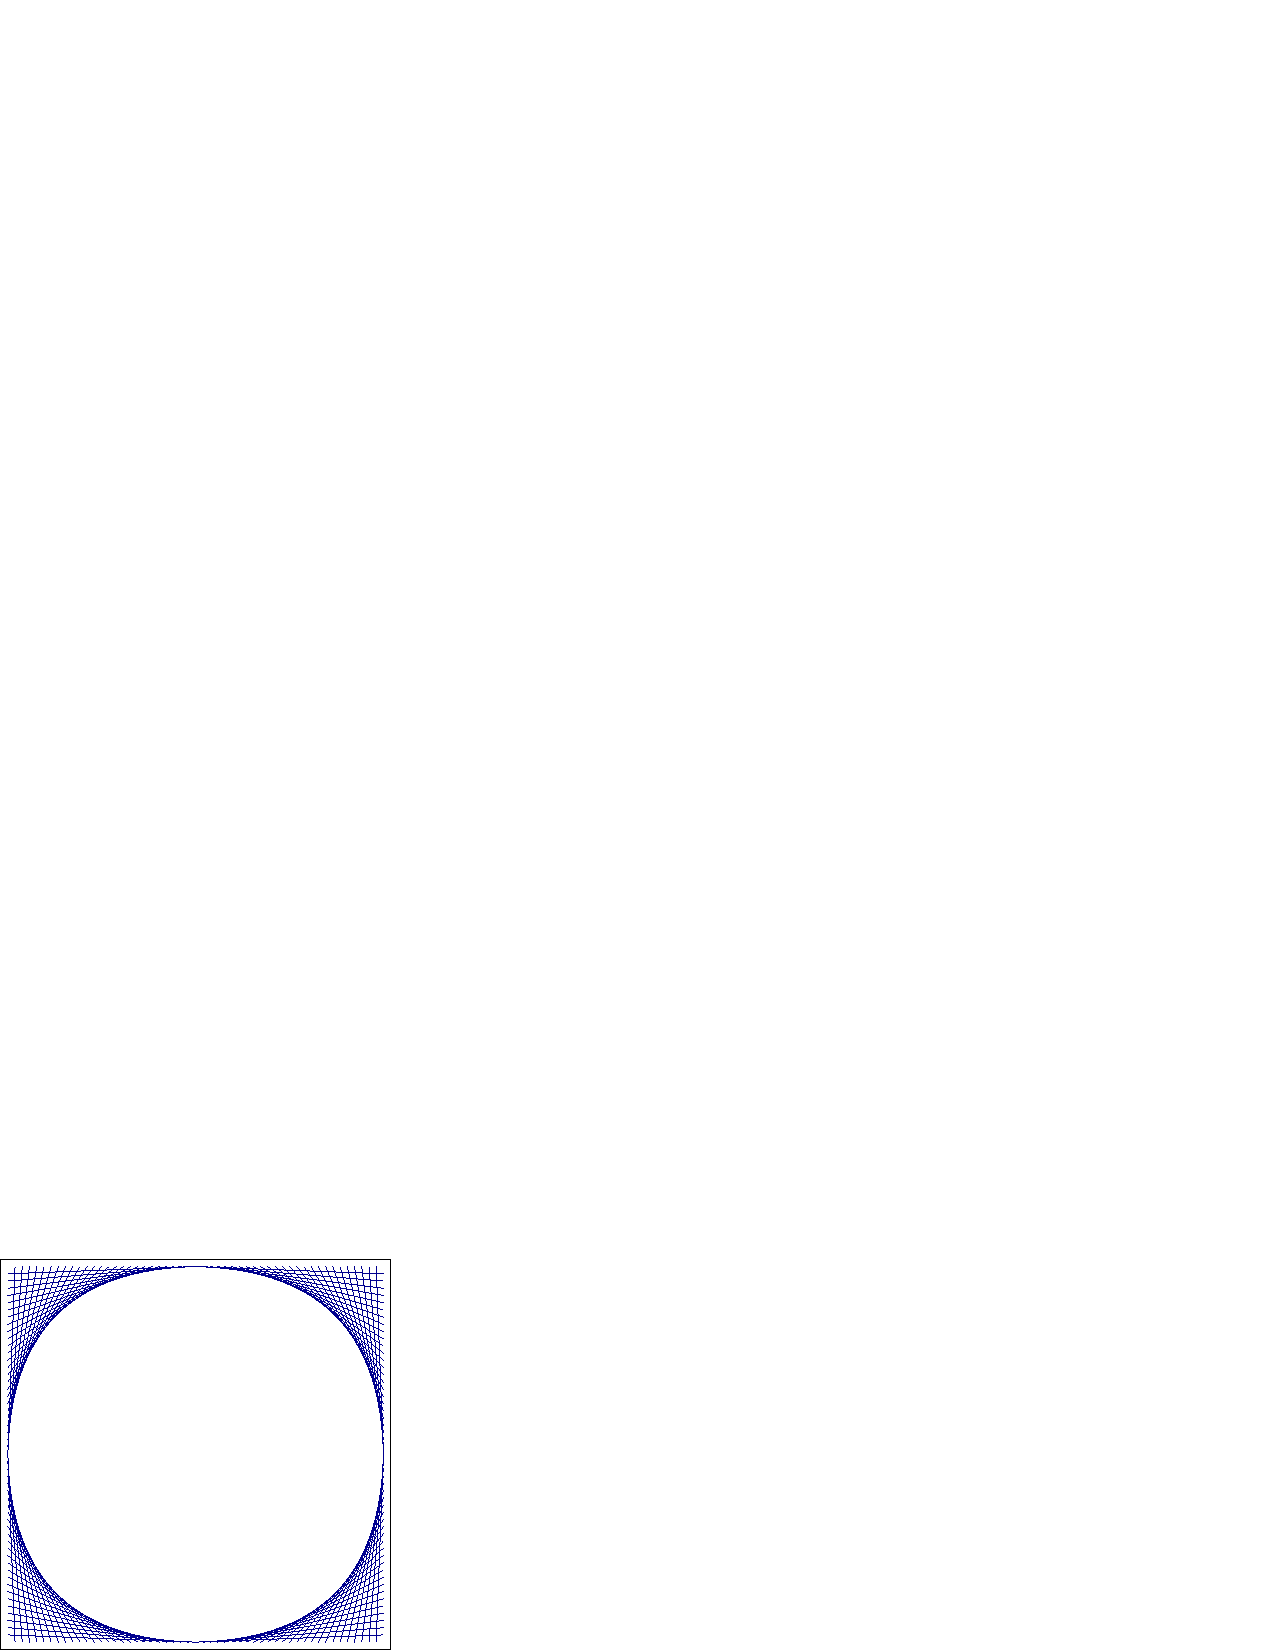
\includegraphics{Arrangement_on_surface_2/fig/fan_grids} &
    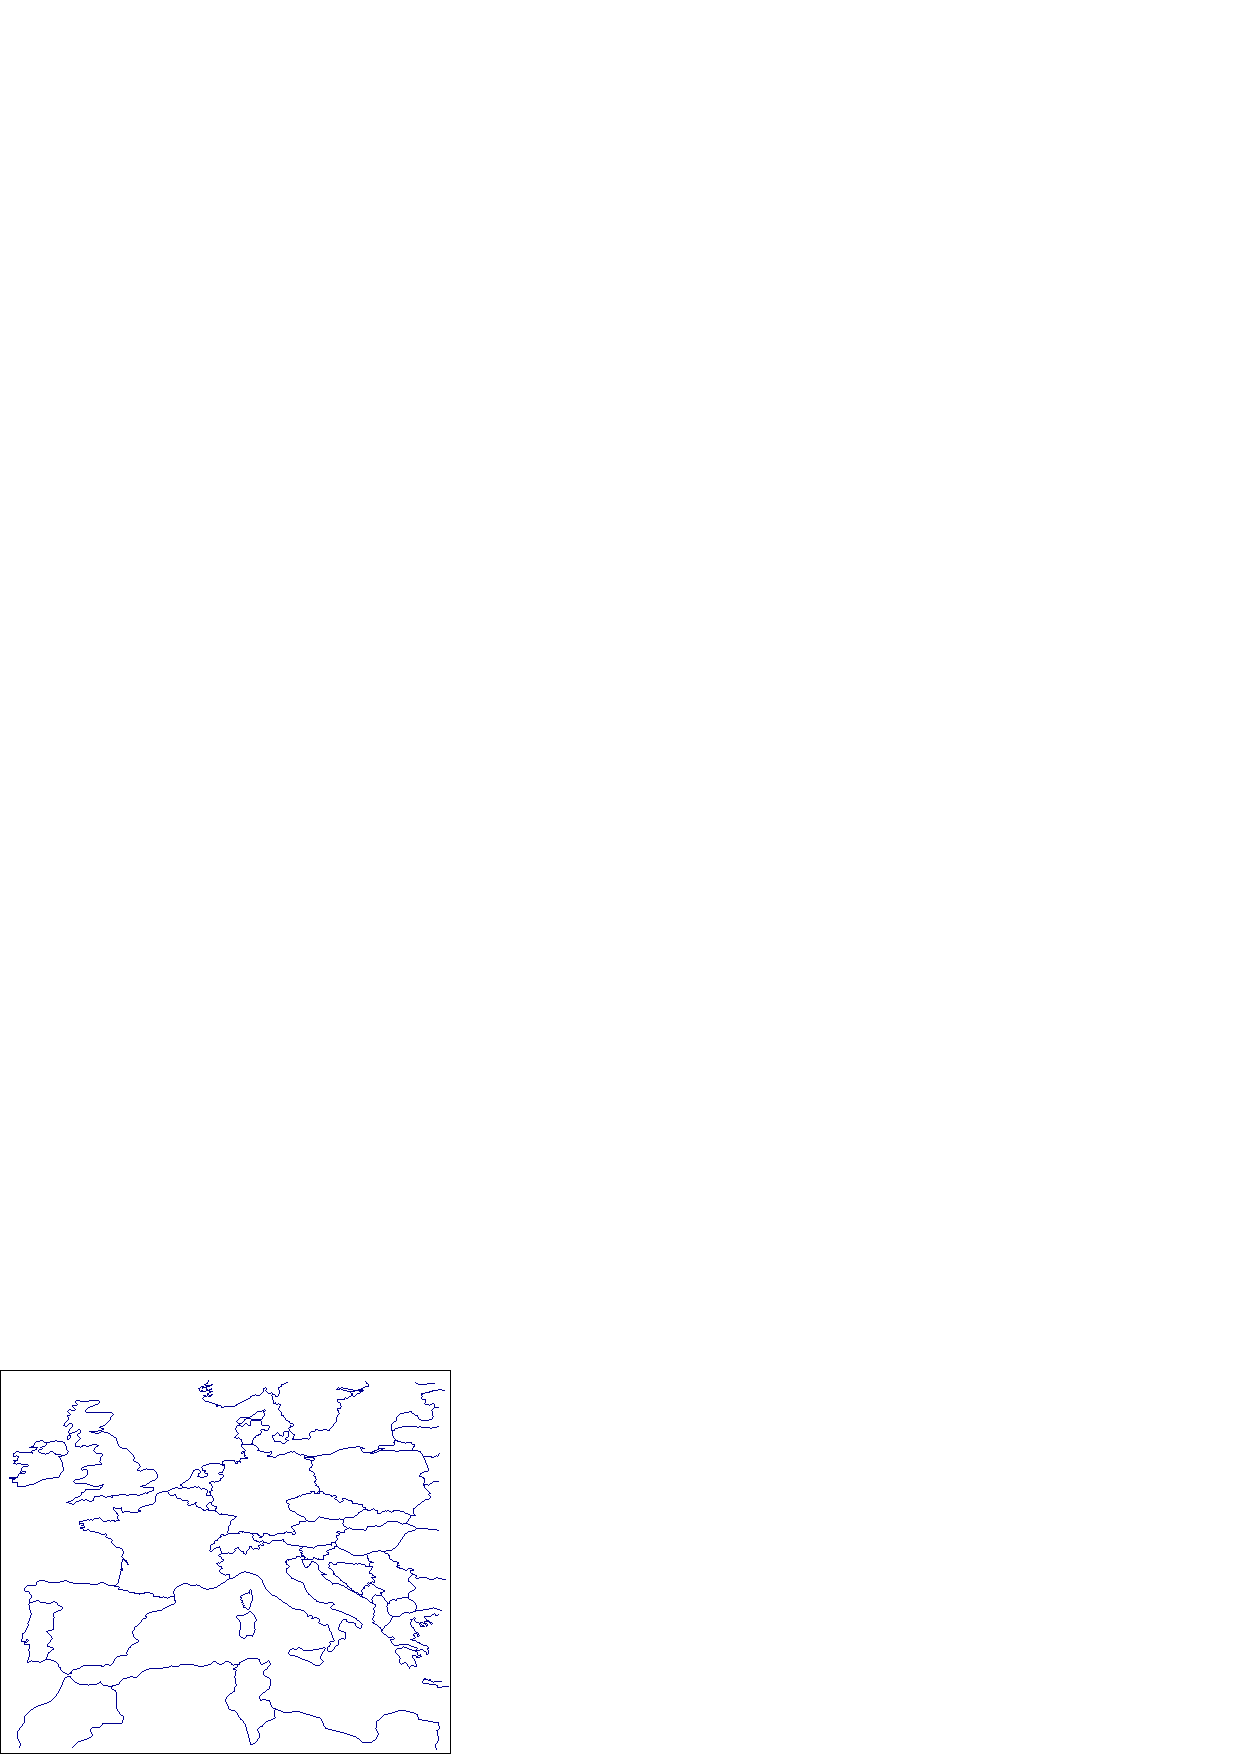
\includegraphics{Arrangement_on_surface_2/fig/Europe} \\
  {\small (a)} & {\small (b)} \\
  \end{tabular}
  \end{center}
\end{ccTexOnly}
\begin{ccHtmlOnly}
  <p><center>
  <table>
  <tr><td><img src="./fig/fan_grids.gif" border=0 alt="fan grids"></td>
      <td><img src="./fig/Europe.gif" border=0 alt="Europe"></td>
  </tr>
  <tr align="center"><td>(a)</td><td>(b)</td></tr>
  </table>
  </center>
\end{ccHtmlOnly}
\caption{(a) An arrangement of $104$ line segments from the input file
\ccc{fan_grids.dat}. (b) An arrangement of more than $3000$ interior
disjoint line segments, defined in the input file
\ccc{Europe.dat}.\label{arr_fig:predef_kernels}}
\end{figure}

In the following example we use the predefined
\ccc{Exact_predicates_exact_constructions_kernel} for instantiating our
segment-traits class. This kernel use interval arithmetic to filter the
exact computations. The program reads a set of line segments with integer
coordinates from a file and computes their arrangement. By default it
opens the \ccc{fan_grids.dat} input-file, located in the examples folder,
which contains $104$ line segments that form four ``fan-like'' grids and
induce a dense arrangement, as illustrated in
Figure~\ref{arr_fig:predef_kernels}(a):

\ccIncludeExampleCode{Arrangement_on_surface_2/predefined_kernel.cpp}

The arrangement package also offers a simpler alternative
segment-traits class. The traits class
\ccc{Arr_non_caching_segment_basic_traits_2<Kernel>} models 
the \ccc{ArrangementBasicTraits_2} concept. It uses
\ccc{Kernel::Point_2} as its point type and
\ccc{Kernel::Segment_2} as its $x$-monotone curve type. As this
traits class does not support intersecting and splitting segments,
the kernel representation is sufficient. It is still less
efficient than \ccc{Arr_segment_traits_2} for constructing
arrangements of pairwise disjoint line segments in many cases, as
it performs no caching at all, but using this traits class may be
preferable as it reduces the memory consumption a bit, since no extra
data is stored with the line segments.

The class \ccc{Arr_non_caching_segment_traits_2<Kernel>} inherits
from \ccc{Arr_non_caching_segment_basic_traits_2<Kernel>} and
extends it to be a model of the \ccc{ArrangementTraits_2} concept.
It may thus be used to construct arrangement of intersecting line
segments, but as explained above, for efficiency reasons it is
recommended to use it only when the arrangement is very sparse and
contains hardly any intersection points.

In the following example we read an input file containing a set of
line segments that are pairwise disjoint in their interior. As the
segments do not intersect, no new points are constructed and we can
instantiate the \ccc{Arr_non_caching_segment_traits_basic_2<Kernel>}
class-template with the predefined
\ccc{Exact_predicates_inexact_constructions_kernel}. Note that we use
the \ccc{insert_non_intersecting_curves()} function to construct the
arrangement.
By default, the example opens the \ccc{Europe.dat} input-file,
located in the examples folder, which contains more than $3000$ line segments
with floating-point coordinates that form the map of Europe, as depicted in
Figure~\ref{arr_fig:predef_kernels}(b):

\ccIncludeExampleCode{Arrangement_on_surface_2/predefined_kernel_non_intersecting.cpp}

The \ccc{Arr_linear_traits_2<Kernel>} class used for demonstrating the
construction of arrangements of unbounded curves is capable of handling
bounded and unbounded linear objects, namely lines, rays and line
segments. It is parameterized by a geometric kernel and such that
its nested \ccc{Point_2} type is the same as the kernel point. The
\ccc{Curve_2} (and \ccc{X_monotone_curve_2}) type it defines is
constructible from a \ccc{Kernel::Line_2}, a \ccc{Kernel::Ray_2} or
from a \ccc{Kernel::Segment_2} object. Just like the default
segment-traits class, the linear-traits class also use caching
techniques to speed up its predicates and constructions.

%------------------------------------------------------------------
\subsection{The Polyline-Traits Class\label{arr_ssec:tr_polylines}}
%------------------------------------------------------------------

The \ccc{Arr_polyline_traits_2<SegmentTraits>} class can be used
to maintain arrangements of polylines (a.k.a. poly-segments),
which are continuous piecewise linear curves. A polyline can be
created from a range of points, where the $i$-th and $(i+1)$-st
points in the range represent the endpoints of the $i$-th segment
of the polyline. The polyline traits class is parameterized with a
segment-traits class that supports the basic operations on
segments.

Polylines are the simplest form of a curves that are not
necessarily $x$-monotone. They can be used to approximate more
complicated curves in a convenient manner, as the algebra needed
to handle them is elementary --- rational arithmetic is sufficient
to construct an arrangement of polylines is an exact and robust
manner. Note, however, that a single polyline can be split into
many $x$-monotone polylines, and that the number of intersection
points (or overlapping sections) between two polylines can also
be large. 

The polyline-traits class is a model of the \ccc{ArrangementTraits_2}
concept and of the \ccc{ArrangementLandmarkTraits_2} concept.
It inherits its point type from the segment-traits class, and defines
the polyline type, which serves as its \ccc{Curve_2}. Polyline curve
objects can be constructed from a range of points. They also enable
the traversal over the range of defining points, whose first and
past-the-end iterators can be obtained through the methods \ccc{begin()}
and \ccc{end()}. The nested \ccc{X_monotone_curve_2} type inherits
from \ccc{Curve_2}. The points in an $x$-monotone curve are
always stored in lexicographically increasing order of their
coordinates.

\begin{figure}[t]
\begin{ccTexOnly}
  \begin{center}
  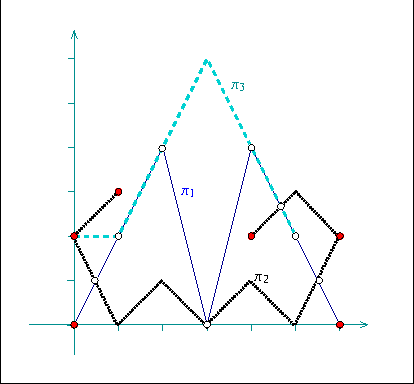
\includegraphics{Arrangement_on_surface_2/fig/ex_12}
  \end{center}
\end{ccTexOnly}
\begin{ccHtmlOnly}
  <p><center>
  <img src="./fig/ex_12.gif" border=0 alt="Example 12">
  </center>
\end{ccHtmlOnly}
\caption{An arrangement of three polylines, as constructed in
\ccc{polylines.cpp}. Disks mark vertices associated with
polyline endpoints, while circles mark vertices that correspond
to intersection points. Note that $\pi_2$ is split into three
$x$-monotone polylines, and that $\pi_1$ and $\pi_3$ have two
overlapping sections.\label{arr_fig:ex_12}}
\end{figure}

The following example program constructs an arrangement of three
polylines, as depicted in Figure~\ref{arr_fig:ex_12}. Note that
most points defining the polylines are not associated with arrangement
vertices. The arrangement vertices are either the extreme points of
each $x$-monotone polyline or the intersection points between two
polylines:

\ccIncludeExampleCode{Arrangement_on_surface_2/polylines.cpp}

%--------------------------------------------------------------
\subsection{A Traits Class for Circular Arcs and Line Segments
  \label{arr_ssec:tr_circ_seg}}
%--------------------------------------------------------------

Circles and circular arcs are the simplest form of non-linear curves.
We handle circles whose centers have rational coordinates and whose
squared radii is also rational. If we denote the circle center by $(x_0,y_0)$
and its radius by $r$, then the equation of the circle --- that is,
$(x - x_0)^2 + (y - y_0)^2 = r^2$ --- has rational coefficients.
The intersection points of two such circles are therefore solutions
of a quadratic equation with rational coefficients, or algebraic numbers
of degree $2$. The same applies for intersection points between such a
rational circle and a line, or a line segment, with rational coefficients
(a line whose equation is $ax + by + c = 0$, where $a$, $b$ and $c$ are
rational). Such numbers can be expressed as $\alpha + \beta\sqrt{\gamma}$,
where $\alpha$, $\beta$ and $\gamma$ are all rational numbers.

Arrangement of circular arcs and of line segment are very useful, as they
occur in many applications. For example, when dilating a polygon by some
radius we obtain a shape whose boundary is comprised of line segments,
which correspond to dilated polygon edges, and circular arcs, which
result from dilated polygon vertices. Using the arrangement of the
boundary curves it is possible, for example, to compute the union of a set
of dilated polygons.

The \ccc{Arr_circle_segment_traits_2<Kernel>} class-template is designed
for efficient handling of arrangements of circular arcs and line segments.
It is parameterized by a geometric kernel, and can handle arrangements of
segments of \ccc{Kernel::Circle_2} objects (full circles are also supported)
or of \ccc{Kernel::Line_2} objects --- namely circular arcs and line segments.
It is important to observe that the nested \ccc{Point_2} type defined by the
traits class, whose coordinates are typically algebraic numbers of degree 2,
is {\em not} the same as the \ccc{Kernel::Point_2} type, which is capable of
representing a point with rational coordinates. The coordinates of a
point are represented using the nested \ccc{CoordNT} number-type.

\begin{figure}[t]
\begin{ccTexOnly}
  \begin{center}
  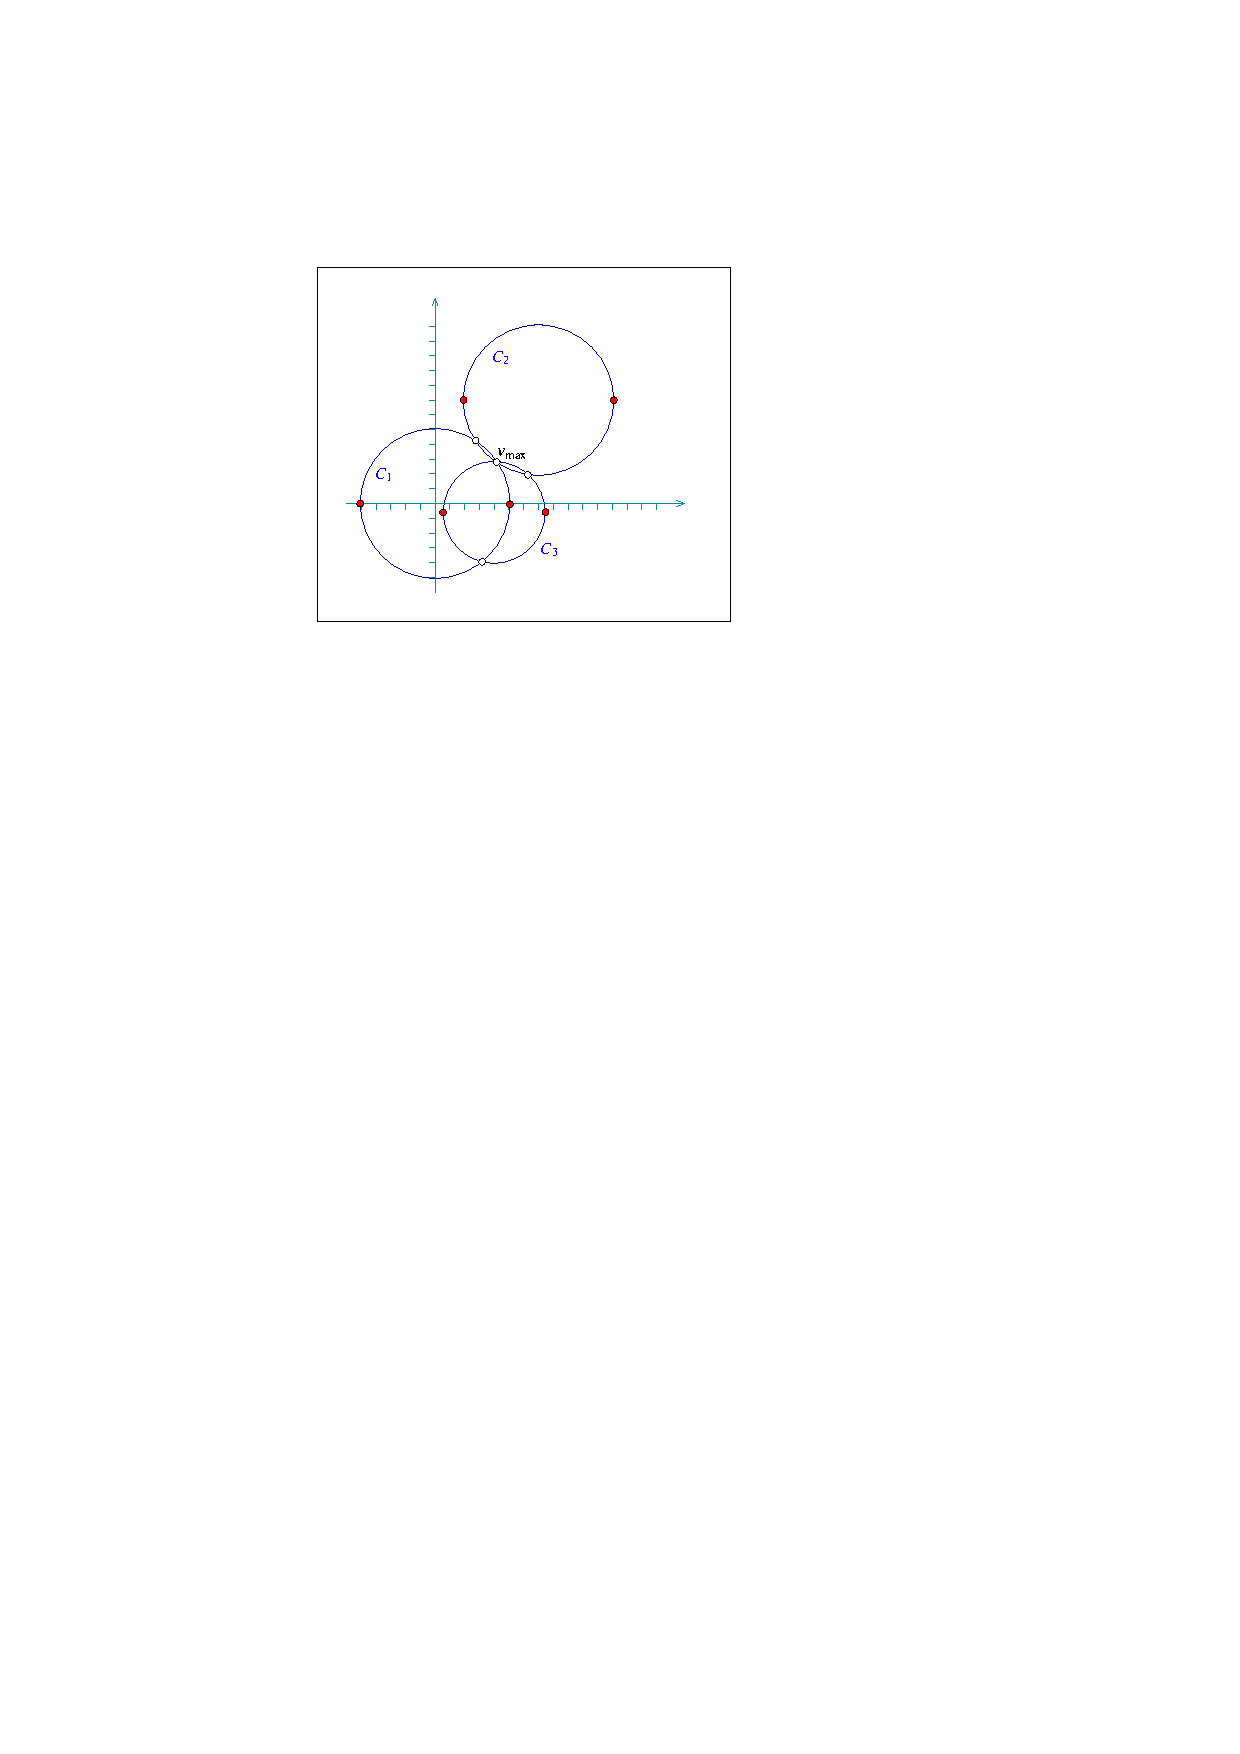
\includegraphics{Arrangement_on_surface_2/fig/ex_13}
  \end{center}
\end{ccTexOnly}
\begin{ccHtmlOnly}
  <p><center>
  <img src="./fig/ex_13.gif" border=0 alt="Example 13">
  </center>
\end{ccHtmlOnly}
\caption{An arrangement of three circles constructed in
\ccc{circles.cpp}. Each circle is split into two $x$-monotone
circular arcs, whose endpoints are drawn as disks. Circles
mark vertices that correspond to intersection points. The vertex
$v_{\rm max}$ is a common intersection point of all three
circles.\label{arr_fig:ex_13}}
\end{figure}

In the following example an arrangement of three full circles is
constructed, as shown in Figure~\ref{arr_fig:ex_13}. Then, the vertex
of maximal degree is searched for. The geometric mapping of this
vertex is the point $(4,3)$, as all three circles intersect at this point
and the associated vertex has six incident edges:

\ccIncludeExampleCode{Arrangement_on_surface_2/circles.cpp}

The \ccc{Curve_2} type nested in \ccc{Arr_circle_segment_traits_2} can be
used to represent circles, circular arcs, or line segments. Curve objects
can therefore be constructed from a \ccc{Kernel::Circle_2} object or from
a \ccc{Kernel::Segment_2} object. A circular arc is typically defined by
a supporting circle and two endpoints, where the endpoints are instances
of the \ccc{Point_2} type, with rational or irrational coordinates. The
orientation of the arc is determined by the orientation of the supporting
circle. Similarly, we also support the construction of lines segments given
their supporting line (of type \ccc{Kernel::Line_2}) and two endpoints, which
may have irrational coordinates (unlike the \ccc{Kernel::Segment_2} type).

Note that the \ccc{Kernel::Circle_2} type represents a circle whose
\emph{squared radius} is rational, where the radius itself may be irrational.
However, if the radius is known to be rational, it is advisable to use it,
for efficiency reasons. It is therefore also possible to construct a circle,
or a circular arc specifying the circle center (a \ccc{Kernel::Point_2}), its
rational radius, and its orientation. Finally, we also support the construction
of a circular arcs that is defined by two endpoints and an arbitrary midpoint
that lies on the arc in between its endpoint. In this case, all three points
are required to have rational coordinates (to be kernel points).

The following example demonstrates the usage of the various construction
methods for circular arcs and line segments. Note the usage of the constructor
of \ccc{CoordNT (alpha, beta, gamma)}, which creates a degree-$2$ algebraic
number whose value is $\alpha + \beta\sqrt{\gamma}$.

\ccIncludeExampleCode{Arrangement_on_surface_2/circular_arcs.cpp}

It is also possible to construct $x$-monotone curve objects, which represent
$x$-monotone circular arcs or line segments, using similar constructors.
Construction from a full circle is obviously not supported. See the Reference
Manual for more details.

The traits class-template
\ccc{Arr_circular_line_arc_traits_2<CircularKernel>} offered by the
arrangement package also handles circular arcs and line segments. It
is an alternative to the \ccc{Arr_circle_segment_traits_2<Kernel>}
class-template. These two class templates, while serve similar
purposes, are based on different concepts, and posses different
characteristics. You are encouraged to experiment with both, compare
their performance, and use the most suitable for your case.

%------------------------------------------------------------------
\subsection{A Traits Class for Conic Arcs\label{arr_ssec:tr_conic}}
%------------------------------------------------------------------

A {\em conic curve} is an algebraic curve of degree 2. Namely, it
is the locus of all points $(x,y)$ satisfying the equation $C:\ r
x^2 + s y^2 + t xy + u x + v y + w = 0$, where the six
coefficients $\langle r, s, t, u, v, w \rangle$ completely
characterize the curve. The sign of the expression $\Delta_{C} = 4
r s - t^2$ determines the type of curve:
\begin{itemize}
\item If $\Delta_{C} > 0$ the curve is an ellipse. A circle is a
special case of an ellipse, where $r = s$ and $t = 0$.
%
\item If $\Delta_{C} = 0$ the curve is a parabola --- an unbounded
conic curve with a single connected branch. When $r = s = t = 0$
we have a line, which can be considered as a degenerate parabola.
%
\item If $\Delta_{C} < 0$ the curve is a hyperbola. That is, it
is comprised of two disconnected unbounded branches.
\end{itemize}

As the arrangement package is suitable for bounded curves, we
consider bounded segments of conic curves, referred to as {\em
conic arcs}. A conic arc $a$ may be either (i) a full ellipse, or
(ii) defined by the tuple $\langle C, p_s, p_t, o \rangle$, where
$C$ is a conic curve and $p_s$ and $p_t$ are two points on $C$
(namely $C(p_s) = C(p_t) = 0$) that define the {\em source} and
{\em target} of the arc, respectively. The arc is formed by
traversing $C$ from the source to the target going in the
orientation specified by $o$, which is typically clockwise or
counterclockwise orientation (but may also be collinear in case of
degenerate conic curves).

We always assume that the conic coefficients $\langle r, s,
t, u, v, w \rangle$ are rational. When dealing with linear curves
(line segments and polylines), similar assumptions guarantee that
all intersection points also have rational coordinates, such that
the arrangement of such curves can be constructed and maintained
using only rational arithmetic. Unfortunately, this does not hold
for conic curves, as the coordinates of intersection points of two
conic curves with rational coefficients are in general algebraic
numbers of degree $4$.\footnote{Namely, they are roots of
polynomials with integer coefficients of degree $4$. However, in
some special cases, for example when handling only circles and
circular arcs, the coordinates of the intersection points are only
of degree $2$, namely they are solutions of quadratic equations.}
In addition, conic arcs may not necessarily be $x$-monotone, and
must be split at points where the tangent to the arc is vertical.
In the general case, such points typically have coordinates that
are algebraic numbers of degree $2$.
It is therefore clear that we have to use different number types
to represent the conic coefficients and the point coordinates.
Note that as arrangement vertices induced by intersection points
and points with vertical tangents are likely to have algebraic
coordinates, we also allow the original endpoints of the input arcs
$p_s$ and $p_t$ to have algebraic coordinates.

The \ccc{Arr_conic_traits_2<RatKernel, AlgKernel, NtTraits>} class
template is designed for efficient handling of arrangements of
bounded conic arcs. The template has three parameters, defined as
follows:
\begin{itemize}
\item The \ccc{RatKernel} class is a geometric kernel, whose field
type is an exact rational type. It is used to define basic
geometric entities (e.g., a line segment or a circle) with rational
coefficients. Typically we use one of the standard \cgal\ kernels,
instantiated with the number type \ccc{NtTraits::Rational} (see
below).
%
\item The \ccc{AlgKernel} class is a geometric kernel whose field
type is an exact algebraic type. It is used to define points with
algebraic coordinates. Typically we use one of the standard
\cgal\ kernels, instantiated with the number type
\ccc{NtTraits::Algebraic} (see below).
%
\item The \ccc{NtTraits} class (the number-type traits class)
encapsulates all the numeric operations needed for performing the
geometric computation carried out by the geometric traits class.
It defines the \ccc{Integer}, \ccc{Rational} and \ccc{Algebraic}
number-types, and supports several operations on these types, such
as conversion between number types, solving quadratic equations
and extracting the real roots of a polynomial with integer
coefficients. It is highly recommended to use the
\ccc{CORE_algebraic_number_traits} class, which is included in the
arrangement package. It relies on the exact number types
implemented in the {\sc Core} library and performs exact
computations on the number types it defines.
\end{itemize}

The \ccc{Arr_conic_traits_2} models the \ccc{ArrangementTraits_2} and
the \ccc{ArrangementLandmarkTraits_2} concepts. (It supports
the landmark point-location strategy). Its \ccc{Point_2} type is
derived from \ccc{AlgKernel::Point_2}, while the \ccc{Curve_2}
type represents a bounded, not necessarily $x$-monotone, conic arc.
The \ccc{X_monotone_curve_2} type is derived from \ccc{Curve_2},
but its constructors are to be used only by the traits class.
You should therefore construct only \ccc{Curve_2} objects and
insert them into the arrangement using the \ccc{insert()}
or \ccc{insert()} functions.

Conic arcs can be constructed from full ellipses or by specifying
a supporting curve, two endpoints and an orientation. However,
several constructors of \ccc{Curve_2} are available to allow for some
special cases, such as circular arcs or line segments. The
\ccc{Curve_2} (and the derived \ccc{X_monotone_curve_2}) classes
also support basic access functions such as \ccc{source()},
\ccc{target()} and \ccc{orientation()}.

%~~~~~~~~~~~~~~~~~~~~~~~~~~~~~~~~~~~~~~~~~~~~~~~~~~
\subsubsection{Examples for Arrangements of Conics}
%~~~~~~~~~~~~~~~~~~~~~~~~~~~~~~~~~~~~~~~~~~~~~~~~~~

\begin{figure}[t]
\begin{ccTexOnly}
  \begin{center}
  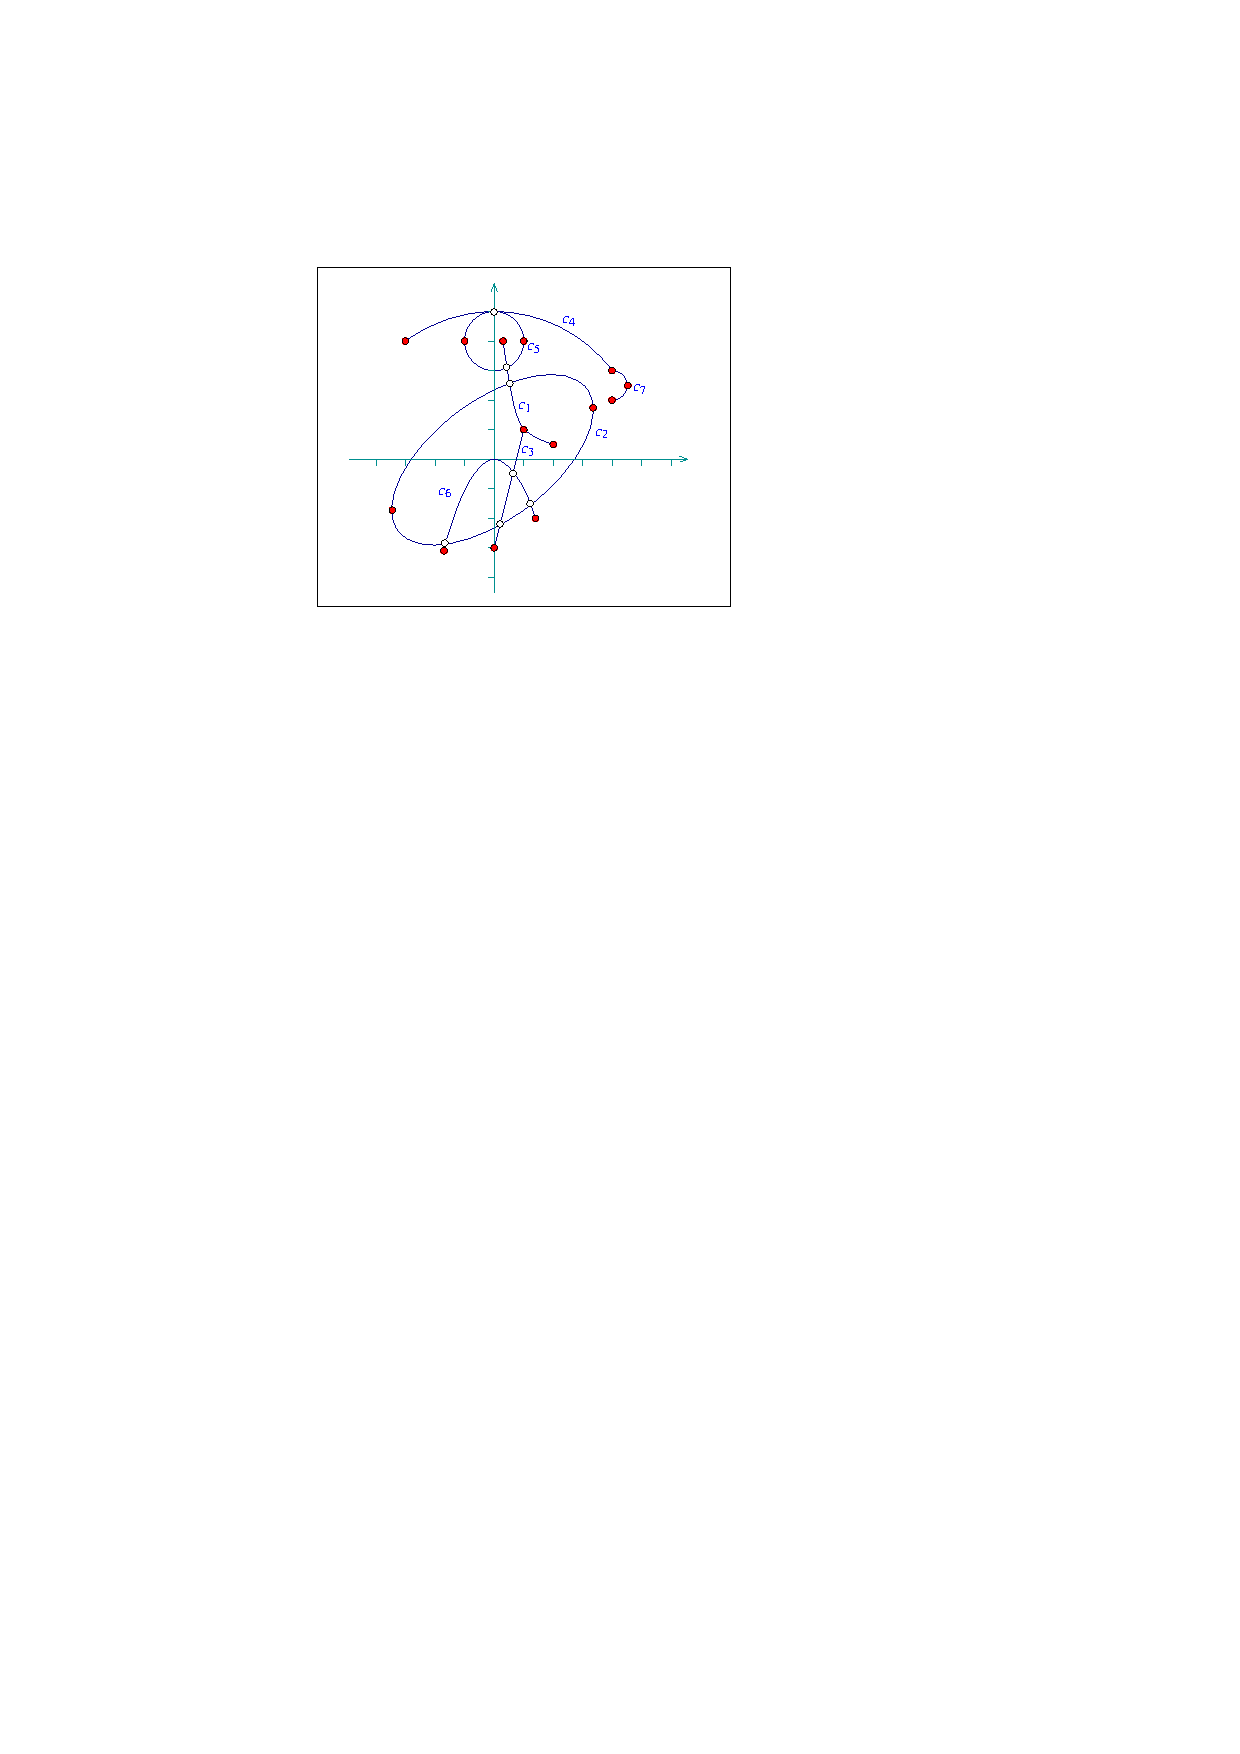
\includegraphics{Arrangement_on_surface_2/fig/ex_14}
  \end{center}
\end{ccTexOnly}
\begin{ccHtmlOnly}
  <p><center>
  <img src="./fig/ex_14.gif" border=0 alt="Example 14">
  </center>
\end{ccHtmlOnly}
\caption{An arrangement of mixed conic arcs, as constructed in
\ccc{conics.cpp}.\label{arr_fig:ex_14}}
\end{figure}

The following example demonstrates the usage of the various
constructors for conic arcs. The resulting arrangement is depicted
in Figure~\ref{arr_fig:ex_14}. Especially noteworthy are the
constructor of a circular arc that accepts three points and the
constructor that allows specifying approximate endpoints, where the
exact endpoints are given explicitly as intersections of
the supporting conic with two other conic curves. Also note that as the
preconditions required by some of these constructors are rather
complicated (see the Reference Manual for the details), a
precondition violation does not cause the program to terminate ---
instead, an {\em invalid} arc is created. We can verify the validity
of an arc by using the \ccc{is_valid()} method. Needless to say, inserting
invalid arcs into an arrangement is not allowed.

\ccIncludeExampleCode{Arrangement_on_surface_2/conics.cpp}

The last example in this section demonstrates how the conic-traits
class can handle intersection points with multiplicity. The
supporting curves of the two arcs, a circle centered at
$(0,\frac{1}{2})$ with radius $\frac{1}{2}$, and the hyperbola $y
= \frac{x^2}{1-x}$,\footnote{This curve can also be written as $C:
x^2 + xy - y = 0$. It is a hyperbola since $\Delta_{C} = -1$.}
intersect at the origin such that the intersection point has
multiplicity $3$ (note that they both have the same horizontal
tangent at $(0,0)$ and the same curvature $1$). In addition, they
have another intersection point at $(\frac{1}{2},\frac{1}{2})$ of
multiplicity $1$:

\ccIncludeExampleCode{Arrangement_on_surface_2/conic_multiplicities.cpp}

%---------------------------------------------------------
\subsection{A Traits Class for Arcs of Rational Functions\label{arr_ssec:tr_ratfunc}}
%---------------------------------------------------------




The traits class  \ccc{Arr_rational_function_traits_2<AlgebraicKernel_d_1>} 
is a model of the \ccc{ArrangementTraits_2}
concept. It handles bounded or unbounded arcs of rational functions,
referred to as {\sl rational arcs} (in particular, such an arc may
correspond to the entire graph of a rational function), and enables the
construction and maintenance of arrangements of such arcs. 
Rational functions, and polynomial functions in particular, are
not only interesting in their own right, they are also very useful
for approximating or interpolating more complicated curves; see,
e.g.,~\cite[Chapter~3]{cgal:ptvf-nrcpp-02}.

A rational function $y = \frac{P(x)}{Q(x)}$ is defined by two polynomials 
$P$ and $Q$ of arbitrary degrees. 
If $Q(x) = 1$ then the function is a simple polynomial function.
Usually the domain is $\R$ but the function may also be 
restricted to a bounded interval $[x_{\rm min}, x_{\rm max}]$ 
or defined over a ray $(-\infty, x_{\rm max}]$ or over $[x_{\rm min}, \infty)$. 
Rational functions are represented by the nested type \ccc{Curve_2}. 
Note that a rational function may be not continuous since roots of $Q$ induce 
vertical asymptotes, which would contradict the notion of an $x$-monotone curve as 
it is introduced by the \ccc{ArrangementTraits_2} concept. 
Thus, continuous portions of rational functions are represented by the nested 
type \ccc{X_monotone_curve_2}, which is different from \ccc{Curve_2}.
Constructors for both classes are provided by the traits. 
A \ccc{Curve_2} may be split up into several \ccc{X_monotone_curve_2}
using \ccc{Make_x_monotone_2}. 

Using the \ccc{Arr_rational_function_traits_2<AlgebraicKernel_d_1>} class
template it is possible to construct and maintain arrangement of
rational arcs.  
The template parameter of the traits must be a model of the 
concept \ccc{AlgebraicKernel_d_1}. 
A rational function is then represented by two polynomials $P$ and $Q$ of type 
\ccc{AlgebraicKernel_d_1::Polynomial_1}. 
A point is represented by a rational function and its $x$-coordinate, which is 
of type \ccc{AlgebraicKernel_d_1::Algebraic_real_1}. 
Note that an explicit representation of the $y$-coordinate is only computed upon 
request, which can be a rather costly operation. 


The constructed rational functions are cached by the traits class. 
The cache is local to each traits class object. 
It is therefore necessary to construct the curves using the constructor 
objects provided by member functions of the traits class. 
%This is also the reason why IO is not handled via the usual stream operators. 
Moreover, a curve must only be used by the traits class object that was 
used to construct it. 
The cache is automatically  cleaned up from time to time.
The amortized clean up costs are constant. 
In addition, there is also a 
separate member function that cleans up the cache on demand.  


\ccc{Arr_rational_function_traits_2<AlgebraicKernel_d_1>} is a model of 
the concepts \ccc{ArrangementTraits_2}, \ccc{ArrangementOpenBoundaryTraits_2},
and \ccc{ArrangementDirectionalXMonotoneTraits_2}; 
the later enables Boolean set operations. 

Note that it is not a model of  \ccc{ArrangementLandmarkTraits_2} concept,
so it is not possible to use the landmark point-location strategy.
%\footnote{This requires a relaxation of \ccc{ArrangementLandmarkTraits_2}, 
%which will be submitted separately.}

\begin{figure}[h] 
\begin{ccTexOnly} 
  \begin{center}
  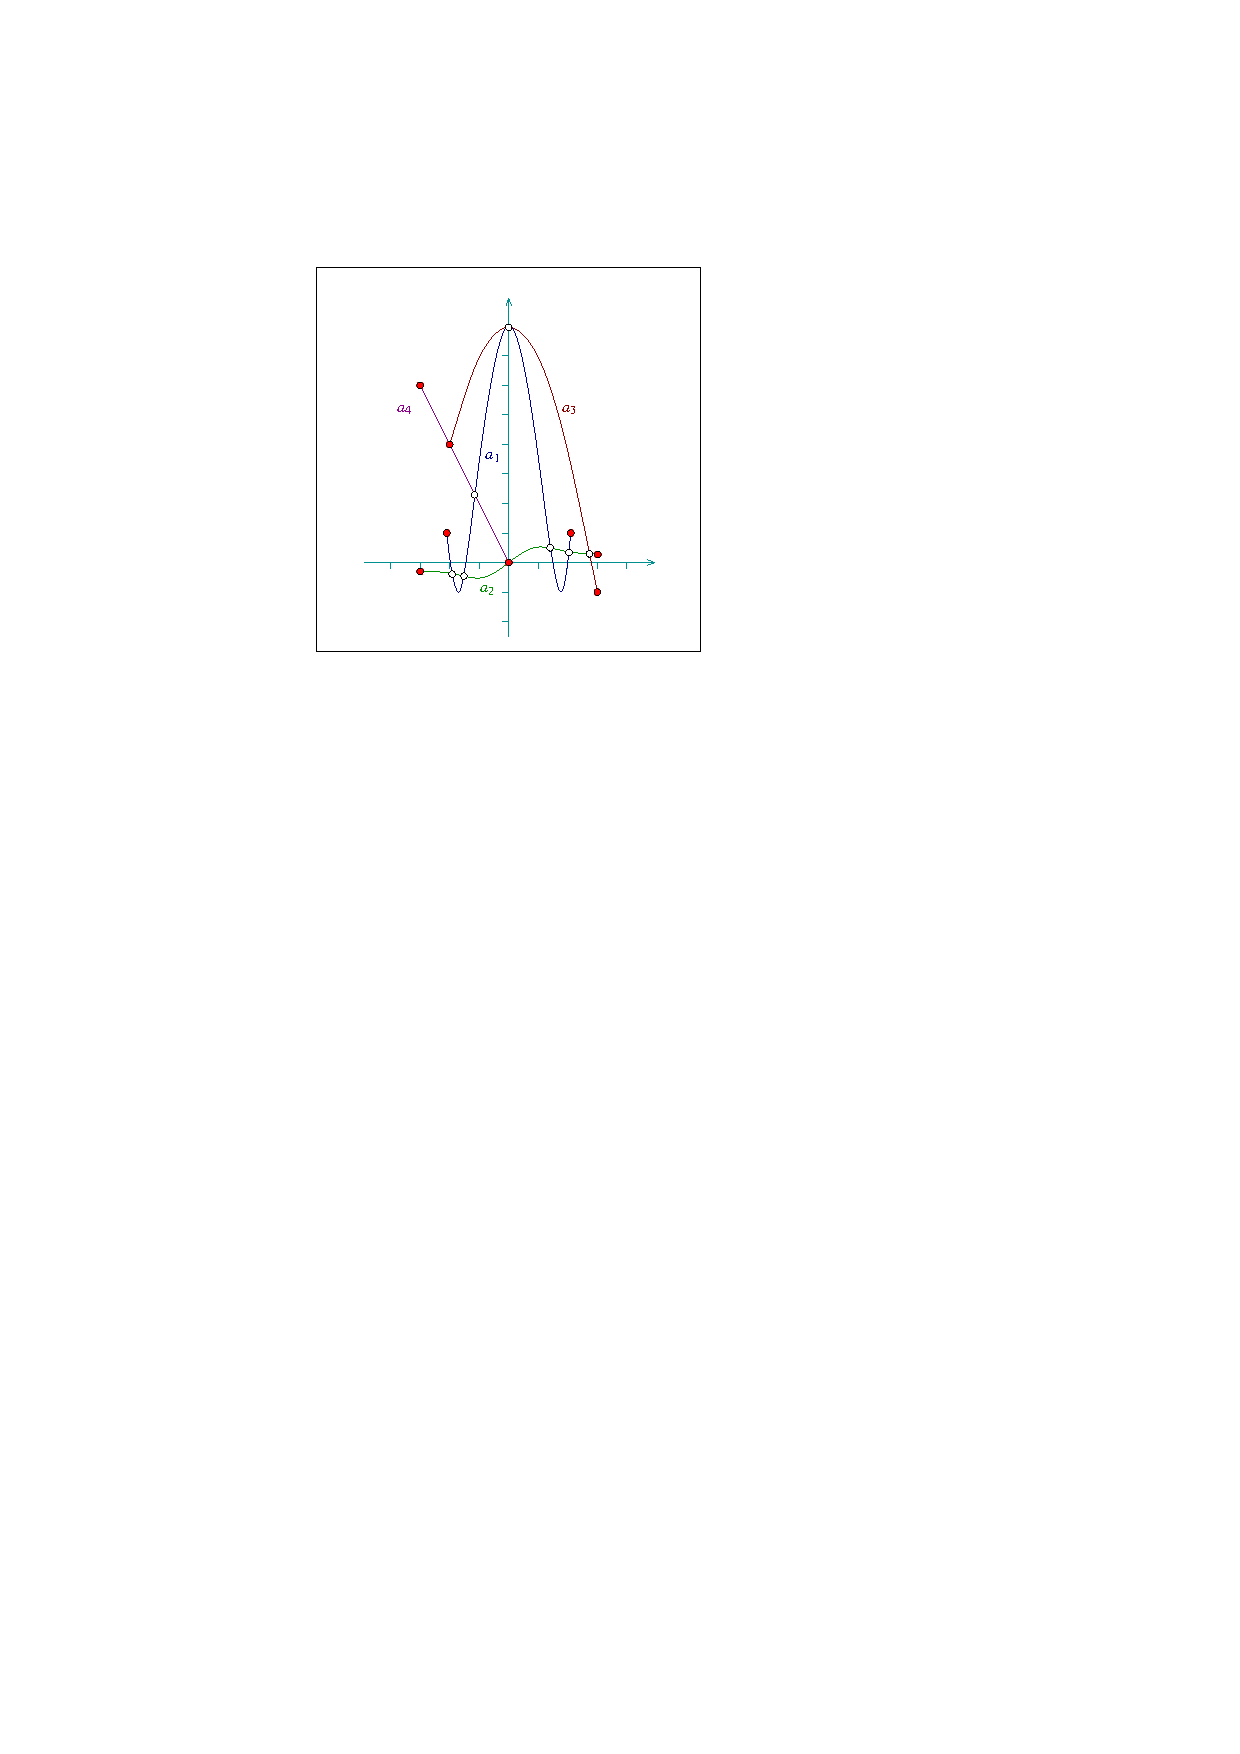
\includegraphics{Arrangement_on_surface_2/fig/ex_16}
  \end{center}
\end{ccTexOnly}
\begin{ccHtmlOnly}
  <p><center>
  <img src="./fig/ex_16.gif" border=0 alt="Example 16">
  </center>
\end{ccHtmlOnly}
\caption{An arrangement of four arcs of rational functions, as
constructed in \ccc{rational_functions.cpp}.\label{arr_fig:ex_16}}
\end{figure}

The following example demonstrates the construction of an
arrangement of rational arcs depicted in
Figure~\ref{arr_fig:ex_16}. Note the usage of the two
constructors, for polynomial arcs and for rational arcs:

\pagebreak[3]

\ccIncludeExampleCode{Arrangement_on_surface_2/rational_functions.cpp}

\begin{figure}[h]
\begin{ccTexOnly}
  \begin{center}
  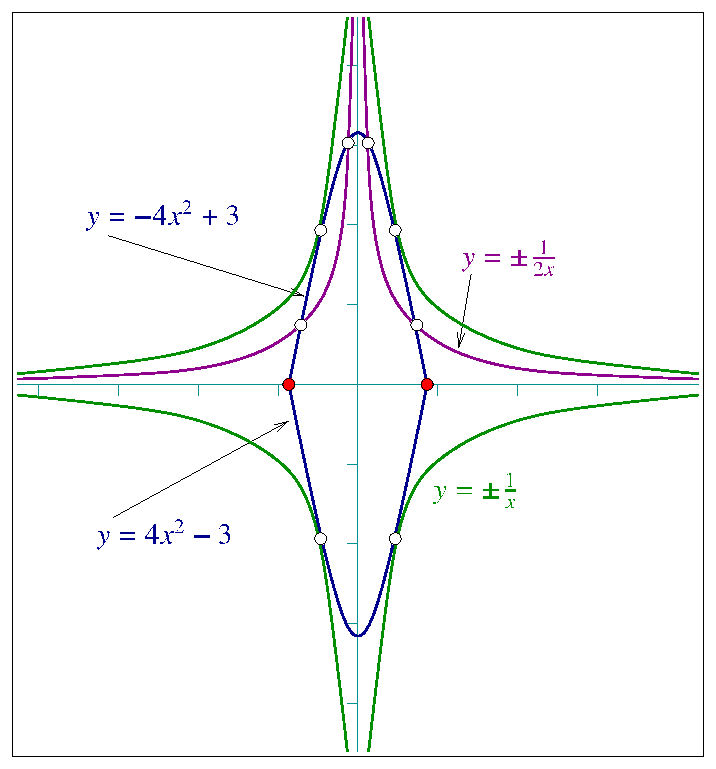
\includegraphics{Arrangement_on_surface_2/fig/ex_unb_rat}
  \end{center}
\end{ccTexOnly}
\begin{ccHtmlOnly}
  <p><center>
  <img src="./fig/ex_unb_rat.gif" border=0 alt="">
  </center>
\end{ccHtmlOnly}
\caption{An arrangement of six arcs of rational functions, as
constructed in
\ccc{unbounded_rational_functions.cpp}.\label{arr_fig:ex_unb_rat}}
\end{figure}

The following example demonstrates the construction of an
arrangement of six rational arcs --- four unbounded arcs and two
bounded ones --- as depicted in Figure~\ref{arr_fig:ex_unb1}. Note
the usage of the constructors of an entire rational function and of
an infinite ``ray'' of such a function. Also observe that the hyperbolas
$y = \pm\frac{1}{x}$ and $y = \pm\frac{1}{2x}$ never intersect, although
they have common vertical and horizontal asymptotes, so very ``thin''
unbounded faces are created between them:

\ccIncludeExampleCode{Arrangement_on_surface_2/unbounded_rational_functions.cpp}

%----------------------------------------------------------------------------
\subsection{A Traits Class for Planar B\'ezier Curves\label{arr_ssec:tr_bez}}
%----------------------------------------------------------------------------

A planar {\em B\'ezier curve} $B$ is a parametric curve defined by a sequence
of {\em control points} $p_0, \ldots, p_n$ as follows:
\begin{eqnarray*}
B(t) = \left(X(t), Y(t)\right)
  = \ccSum{k=0}{n}{p_k \cdot \frac{n!}{k! (n-k)!} \cdot
                   t^k (1-t)^{n-k}}\ .
\end{eqnarray*}
where $t \in [0, 1]$. The degree of the curve is therefore $n$ ---
namely, $X(t)$ and $Y(t)$ are polynomials of degree $n$. B\'ezier curves
have numerous applications in computer graphics and solid modelling. They
are used, for example, in free-form sketches and for defining the true-type
fonts.

Using the \ccc{Arr_Bezier_curve_traits_2<RatKernel, AlgKernel, NtTraits>}
class template it is possible to construct and maintain arrangements of
B\'ezier curves that are given by rational control points (a sequence
of objects of the \ccc{RatKernel::Point_2} type). We can handle curves
of arbitrary degree (in general, a sequence of $n+1$ control points define a 
B\'ezier curve of degree $n$). The template parameters are the same ones
used by the \ccc{Arr_conic_traits_2} class template, and here it is also
recommended to use the \ccc{CORE_algebraic_number_traits} class, with
Cartesian kernels instantiated with the \ccc{Rational} and \ccc{Algebraic}
number-types defined by this class.

As mentioned above, we assume that the coordinates of all control
points that define a B\'ezier curve are rational numbers, so both $X(t)$
and $Y(t)$ are polynomials with rational coefficients. The intersection
points between curves are however algebraic numbers, and their exact
computation is time-consuming. The traits class therefore contains a layer
of geometric filtering that performs all computation in an approximate
manner whenever possible. Thus, it resorts to exact computations only when
the approximate computation fails to produce an unambiguous result.
Note that most arrangement vertices are therefore associated with approximated
points. You cannot access the coordinates of such points and obtain them as
algebraic numbers, and only access to the approximate coordinates in possible.
See the Reference Manual for the exact interface of the \ccc{Point_2},
\ccc{Curve_2} and \ccc{X_monotone_curve_2} defined by the traits class.

The \ccc{Arr_Bezier_curve_traits_2} is a model of the
\ccc{ArrangementTraits_2} concept (but not of the
\ccc{ArrangementLandmarkTraits_2} concept, so it is not possible
to use the landmark point-location strategy for arrangements of
rational arcs).

\begin{figure}[t]
\begin{ccTexOnly}
  \begin{center}
  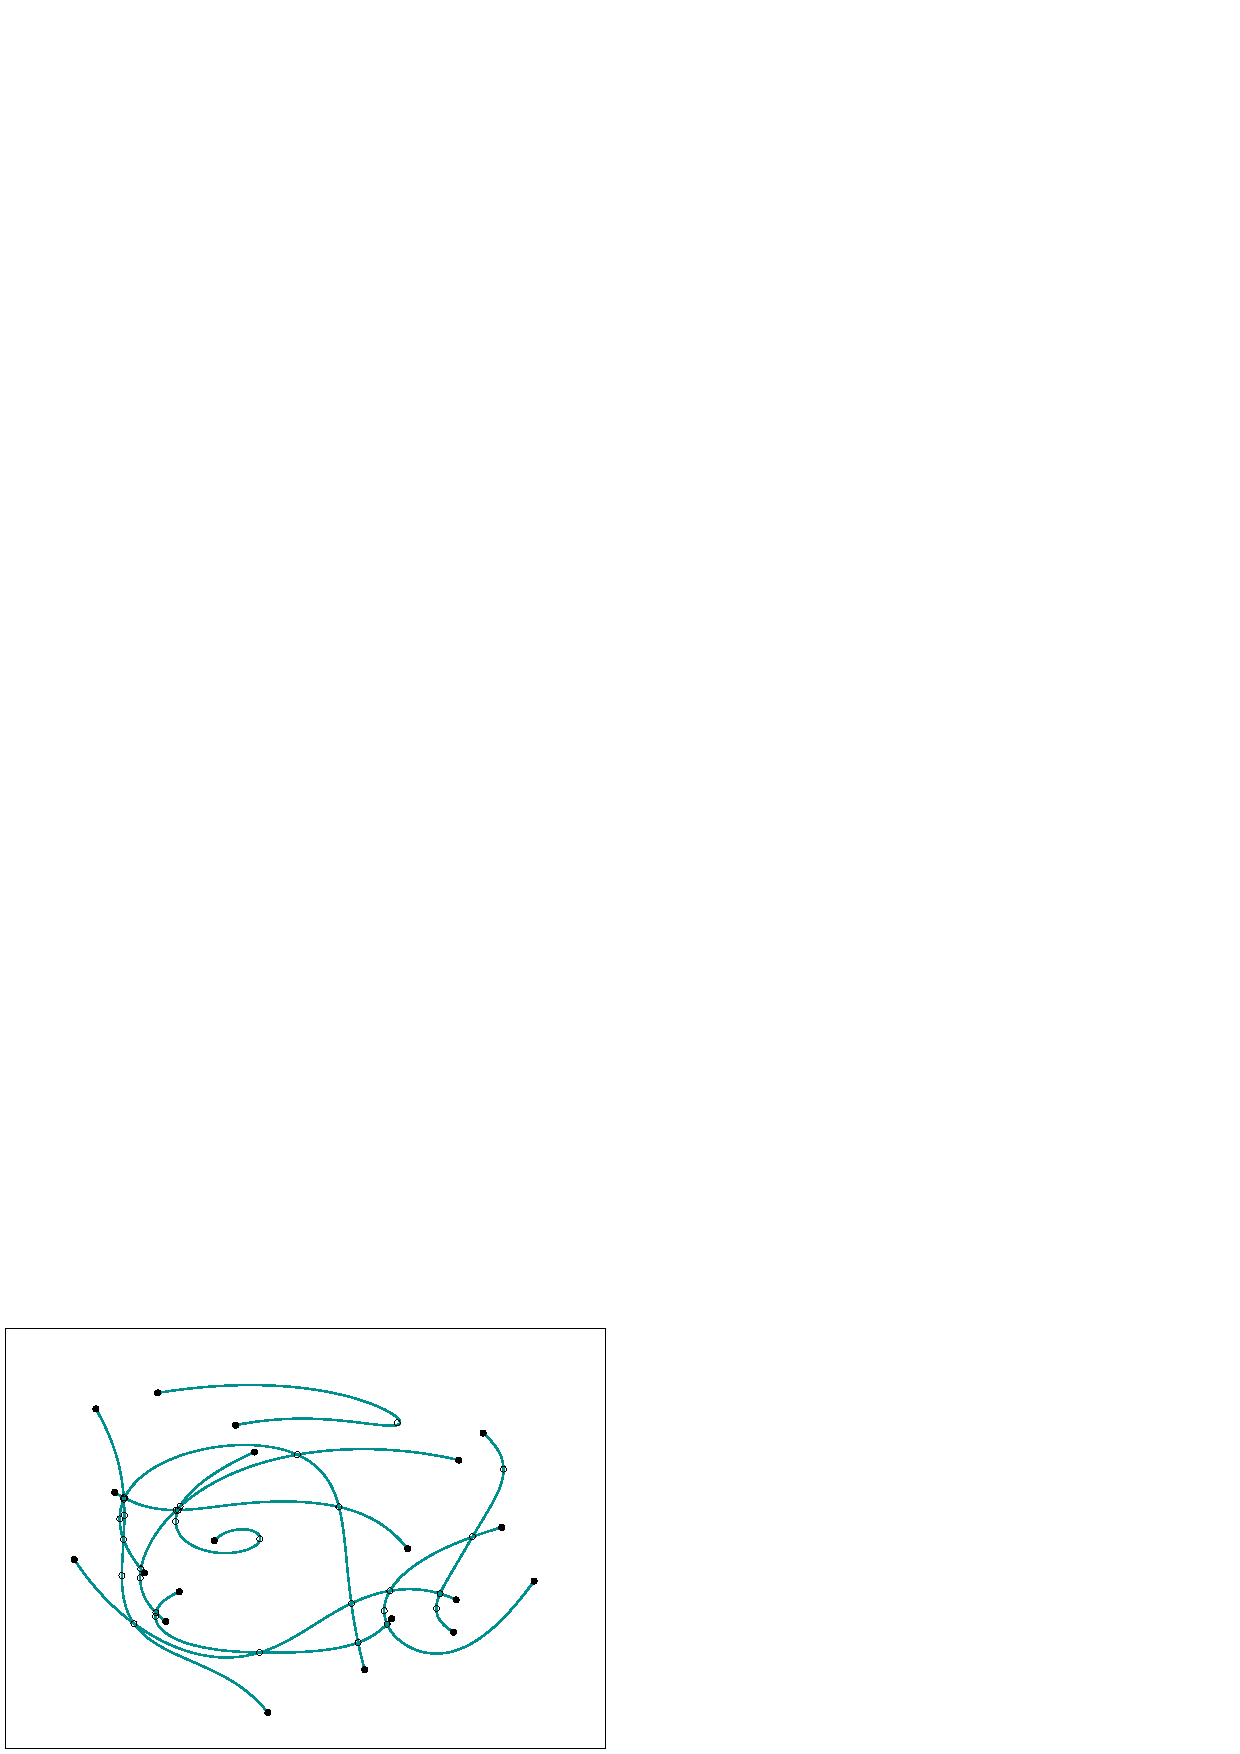
\includegraphics{Arrangement_on_surface_2/fig/Bezier_arr}
  \end{center}
\end{ccTexOnly}
\begin{ccHtmlOnly}
  <p><center>
  <img src="./fig/Bezier_arr.gif" border=0 alt="An arrangement of Bezier curves">
  </center>
\end{ccHtmlOnly}
\caption{An arrangement of ten B\'ezier curves of degree $5$, as
constructed in \ccc{Bezier_curves.cpp}.\label{arr_fig:ex_bez}}
\end{figure}

The following example reads a set of B\'ezier curves from an input
file, where each file is specified by an integer stating its number
of control points, followed by the sequence of control points, given
in integer or rational coordinates. By default, the program uses
the \ccc{Bezier.dat} file, which contains ten curves of degree $5$
each; their resulting arrangement is depicted in
Figure~\ref{arr_fig:ex_bez}.

\ccIncludeExampleCode{Arrangement_on_surface_2/Bezier_curves.cpp}

%-------------------------------------------------------------------------
\subsection{A Traits Class for Planar Algebraic Curves of Arbitrary Degree
  \label{arr_ssec:tr_alg}}
%-------------------------------------------------------------------------

An algebraic curve $C$ in the plane is defined as the (real) zero locus
of a polynomial $f(x,y)$ in two variables. The curve is uniquely defined
by $f$ (although several polynomials might define the same curve). 
We call $f$ a \emph{defining polynomial} of $C$.

% When talking about algebraic curves, we use the term ``segment'' for a
% closed continuous subset of an algebraic curve
% such that each interior point can be parameterized uniquely, as a function in
% $x$ or $y$. In other words, there is no self-intersection in the interior
% of a segment. A weakly $x$-monotone segment is therefore a segment that is
% either vertical, or permits a unique parameterization
We consider arrangements induced by algebraic curves
or by (weakly) $x$-monotone segments for algebraic curves
(Such a segment is not necessarily the maximal possible 
(weakly) x-monotone segment; see below.)
When talking about algebraic curves, 
we use the term ``segment'' for a continuous, possibly non-linear subset 
of an algebraic curve~-- see the definition below.
There are no restrictions on the algebraic curve, that means, 
we support unbounded curves, vertical curves or segments, and isolated points.

The \ccc{Arr_algebraic_segment_traits_2<Coefficient>} class template 
is a model of the \ccc{ArrangementTraits_2} concept (but not of the
\ccc{ArrangementLandmarkTraits_2} concept, so it is not possible
to use the landmark point-location strategy for arrangements of
algebraic curves).
The template argument \ccc{Coefficient} determines 
the type of the scalar coefficients of the polynomial. 
Currently supported types are \ccc{leda_integer}, \ccc{CORE::BigInt}, 
and any instance of \ccc{CGAL::Sqrt_extension<A,B>} 
instantiated with one of the integral types above.

The traits class defines a type \ccc{Curve_2} for algebraic curves.
Such a type can be constructed by the \ccc{Construct_curve_2} functor,
which accepts an instance of \ccc{Polynomial_2} as an argument.
This polynomial type is also available by the traits class 
and constitutes a valid model
of the concept \ccc{Polynomial_d} with two variables (see~??).
%The \ccc{Construct_curve_2} functor performs a topological-geometric analysis
%of the defined curve, and caches the result internally.

\begin{figure}[t]
\begin{ccTexOnly}
  \begin{center}
  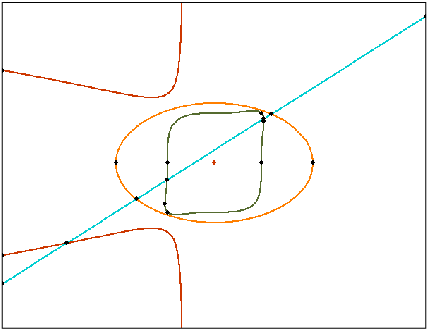
\includegraphics[width=8cm]{Arrangement_on_surface_2/fig/algebraic_curves}
  \end{center}
\end{ccTexOnly}
\begin{ccHtmlOnly}
  <p><center>
  <img src="./fig/algebraic_curves.gif" border=0 alt="An arrangement of algebraic curves">
  </center>
\end{ccHtmlOnly}
\caption{An arrangement of algebraic curves of degrees $1$, $2$, $3$, and $6$,
as constructed in \ccc{algebraic_curves.cpp}.\label{arr_fig:ex_alg_curves}}
\end{figure}

The following examples computes the arrangement induced by the four curves
in Figure~\ref{arr_fig:ex_alg_curves}

\ccIncludeExampleCode{Arrangement_on_surface_2/algebraic_curves.cpp}

We first give a precise definition of segments of algebraic curves.
A point $p$ on a curve $C_f\subset\mathbb{R}^2$ 
(with $f$ its defining equation) is called
\emph{semi-regular}, if locally around $p$, $C_f$ can be written as
a function graph of some continuous function in $x$ or in $y$
(we also say that $p$ is parameterizable in $x$ or $y$, respectively).
The only two cases of non-semi-regular points are isolated points, and
self-intersections. 
A \emph{segment} of a curve is a closed and continuous point set 
such that each interior point is semi-regular.
It follows that a weakly $x$-monotone segment is either a completely vertical
segment, or a segment whose interior points are all parameterizable in $x$.

The traits class allows to construct weakly $x$-monotone segments of a curve
using the \ccc{Construct_x_monotone_segment_2} functor.
The \ccc{X_monotone_curve_2} type of the traits class represents
weakly $x$-monotone segments of a curve; however,
segments may need to be further subdivided into several (sub-)segments,
for technical reasons. Therefore, \ccc{Construct_x_monotone_segment_2}
constructs a sequence of \ccc{X_monotone_curve_2} objects, whose union
represents the weakly $x$-monotone segment that was queried.
We call a segment \emph{terminal} if it can be represented
by the type \ccc{X_monotone_curve_2}.

\begin{ccAdvanced}
The subdivision of segments is due to the internal representation of 
$x$-monotone segments, which is based on a vertical decomposition.
We assume the defining polynomial $f$ of the curve $C$
to be \emph{square-free}, that means, it contains no divisor $g^2$ of total
degree greater than zero. We define a \emph{(complex) critical point}
$p\in\mathbb{C}^2$ by
%
$$f(p)=0=\frac{\partial f}{\partial y}(p).$$
%
An $x$-coordinate $\alpha\in\mathbb{R}$ is \emph{critical}
if either some critical point has $x$-coordinate $\alpha$,
or if the leading coefficient of $f$, considered as a polynomial in $y$,
vanishes. In particular, vertical lines of and isolated point of $C$
can only take place at critical $x$-coordinates.
Between two consecutive critical $x$-coordinates, the curve decomposes
into a finite number of $x$-monotone segments (the same is true on the left
of the leftmost, and on the right of the rightmost critical $x$-coordinate).
The type \ccc{X_monotone_curve_2} is only able to represent such segments
(and sub-segments of them). See Figure~\ref{arr_fig:cylindrical_decomposition} 
for an example of a decomposition into terminal segments. Formally, 
a terminal segment is a weakly $x$-monotone segment that is either vertical, or
its $x$-range contains no critical point in its interior.

\end{ccAdvanced}

\begin{figure}[t]
\begin{ccTexOnly}
 \begin{center}
 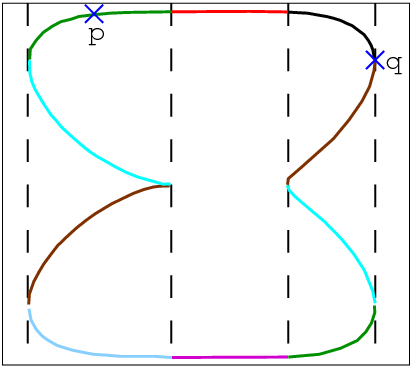
\includegraphics[width=8cm]{Arrangement_on_surface_2/fig/cylindrical_decomposition}
 \end{center}
\end{ccTexOnly}
\begin{ccHtmlOnly}
 <p><center>
 <img src="./fig/cylindrical_decomposition.gif" border=0 alt="The braic curves">
 </center>
\end{ccHtmlOnly}
\caption{The critical $x$-coordinates of an algebraic curve (dashed lines),
         and its decomposition into terminal segments (in different colors).
         The segment from $p$ to $q$ consists of the union of 
         three terminal segments.
         \label{arr_fig:cylindrical_decomposition}}
\end{figure}

Coordinates of points are represented by the type \ccc{Algebraic_real_1},
which is defined in the traits class. 
This type is taken from a model of the \ccc{AlgebraicKernel_1} concept,
which is also available by the type \ccc{Algebraic_kernel_1}.
One can use this model to create algebraic numbers as roots of univariate
polynomials, and process them, for instance, 
compare them, or approximate them to any precision. See the documentation
of \ccc{AlgebraicKernel_1} for more information.
One can construct an object of type \ccc{Point_2} by a triple
($x_0$,cv,i), which means that the $i$-th point (counted from below)
in the fiber of cv at the $x$-coordinate $x_0$ is constructed.
This is also how points are presented internally. 
In the example displayed in Figure~\ref{arr_fig:cylindrical_decomposition},
if $x_1$ denotes the $x$-coordinate of $p$, and $cv$ represents the algebraic
curve, then $p$ could be represented by $(x_1,cv,3)$. If $x_2$
is the $x$-coordinate of $q$, 
then $(x_2,cv,1)$ is a valid representation of $q$.
Although the $y$-coordinate of an object of type \ccc{Point_2} can be queried,
we recommend to be careful with that option, since computing an explicit
representation of the $y$-coordinate as an \ccc{Algebraic_real_1} object
can become rather expensive.

\begin{figure}[t]
\begin{ccTexOnly}
 \begin{center}
 
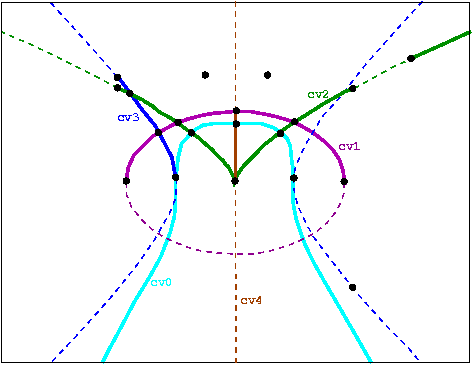
\includegraphics[width=8cm]{Arrangement_on_surface_2/fig/algebraic_segments}
 \end{center}
\end{ccTexOnly}
\begin{ccHtmlOnly}
 <p><center>
 <img src="./fig/algebraic_segments.gif" border=0 alt="An arrangement of algebraic segments">
 </center>
\end{ccHtmlOnly}
\caption{An arrangement of algebraic segments (solid lines),
as constructed in \ccc{algebraic_segments.cpp}. The supporting curves
are drawn in dashed lines.\label{arr_fig:ex_alg_segments}}
\end{figure}

The following code exemplifies various methods to construct
algebraic segments. The computed arrangement is displayed in
Figure~\ref{arr_fig:ex_alg_segments}.

\ccIncludeExampleCode{Arrangement_on_surface_2/algebraic_segments.cpp} 

%-----------------------------------------------------------
\subsection{Traits-Class Decorators\label{arr_ssec:meta_tr}}
%-----------------------------------------------------------

Geometric traits-class decorators allow you to attach auxiliary
data to curves and to points. The data is automatically manipulated 
by the decorators and distributed to the constructed geometric entities. 
Note that additional information can alternatively be maintained by extending 
the vertex, halfedge, or face types provided by the \dcel\ class used 
by the arrangement; see the details in Section~\ref{arr_sec:ex_dcel}.

The arrangement package includes a generic traits-class decorator
template named 
\ccc{Arr_curve_data_traits_2<BaseTraits, XMonotoneCurveData, Merge, CurveData, Convert>}.
This decorator is used to attach a data field to curves and to
$x$-monotone curves. It is parameterized by a base-traits class, which is
one of the geometric traits classes described in the previous subsections, or
a user-defined traits class. The curve-data decorator derives itself from the
base-traits class, and in particular inherits its \ccc{Point_2} type.
In addition:
\begin{itemize}
\item \ccc{Curve_2} is derived from the basic \ccc{BaseTraits::Curve_2}
class, extending it by an extra field of type \ccc{CurveData}.
%
\item \ccc{X_monotone_curve_2} is derived from the basic
\ccc{BaseTraits::X_monotone_curve_2} class, extending it by an extra field of
type \ccc{XMonotoneCurveData}.
\end{itemize}
Note that the \ccc{Curve_2} and \ccc{X_monotone_curve_2} are not
the same, even if the \ccc{BaseTraits::Curve_2} and
\ccc{BaseTraits::X_monotone_curve_2} are (as in the case of the 
segment-traits class for example). The extended curve types support the
additional methods \ccc{data()} and \ccc{set_data()} for
accessing and modifying the data field.

You can create an extended curve (or an extended $x$-monotone curve)
from a basic curve and a curve-data object. When curves are
inserted into an arrangement, they may be split, and the
decorator handles their data fields automatically:
\begin{itemize}
\item When a curve is subdivided into $x$-monotone subcurves, its
data field of type \ccc{CurveData} is converted to an \ccc{XMonotoneCurveData}
object $d$ using the \ccc{Convert} functor. The object $d$ is automatically
associated with each of the resulting $x$-monotone subcurves.

Note that by default, the \ccc{CurveData} type is identical to the
\ccc{XMonotoneCurveData} type (and the conversion functor \ccc{Convert}
is trivially defined). Thus, the data field associated with the original
curve is just duplicated and stored with the $x$-monotone subcurves.
%
\item When an $x$-monotone curve is split into two, the decorator
class automatically copies its data field to both resulting subcurves.
%
\item When intersecting two $x$-monotone curves $c_1$ and $c_2$, the
result may include overlapping sections, represented as
$x$-monotone curves. In this case the data fields of $c_1$ and $c_2$
are merged into a single \ccc{XMonotoneCurveData} object,
using the \ccc{Merge} functor, which is supplied as a
parameter to the traits class-template. The resulting object is
assigned to the data field of the overlapping subcurves.
%
\item Merging two $x$-monotone curves is allowed only when (i)~the two
curves are geometrically mergeable --- that is, the base-traits class
allows to merge them --- and (ii)~the two curves store the same data field.
\end{itemize}

The \ccc{Arr_consolidated_curve_data_traits_2<BaseTraits, Data>} decorator
specializes the generic curve-data decorator. It extends the basic
\ccc{BaseTraits::Curve_2} by a single \ccc{Data} field, and the basic
\ccc{BaseTraits::X_monotone_curve_2} with a {\em set} of (distinct) data 
objects. The \ccc{Data} type is required to support the equality operator, 
used to ensure that each set contains only distinct data objects with no 
duplicates.
When a curve with a data field $d$ is subdivided into $x$-monotone subcurves,
each subcurve is associated with a set $S = \{ d \}$. In case of an overlap
between two $x$-monotone curves $c_1$ and $c_2$ with associated data sets
$S_1$ and $S_2$, respectively, the overlapping subcurve is associated with
the consolidated set $S_1 \cup S_2$.

%~~~~~~~~~~~~~~~~~~~~~~~
\subsubsection{Examples}
%~~~~~~~~~~~~~~~~~~~~~~~

\begin{figure}[t]
\begin{ccTexOnly}
  \begin{center}
  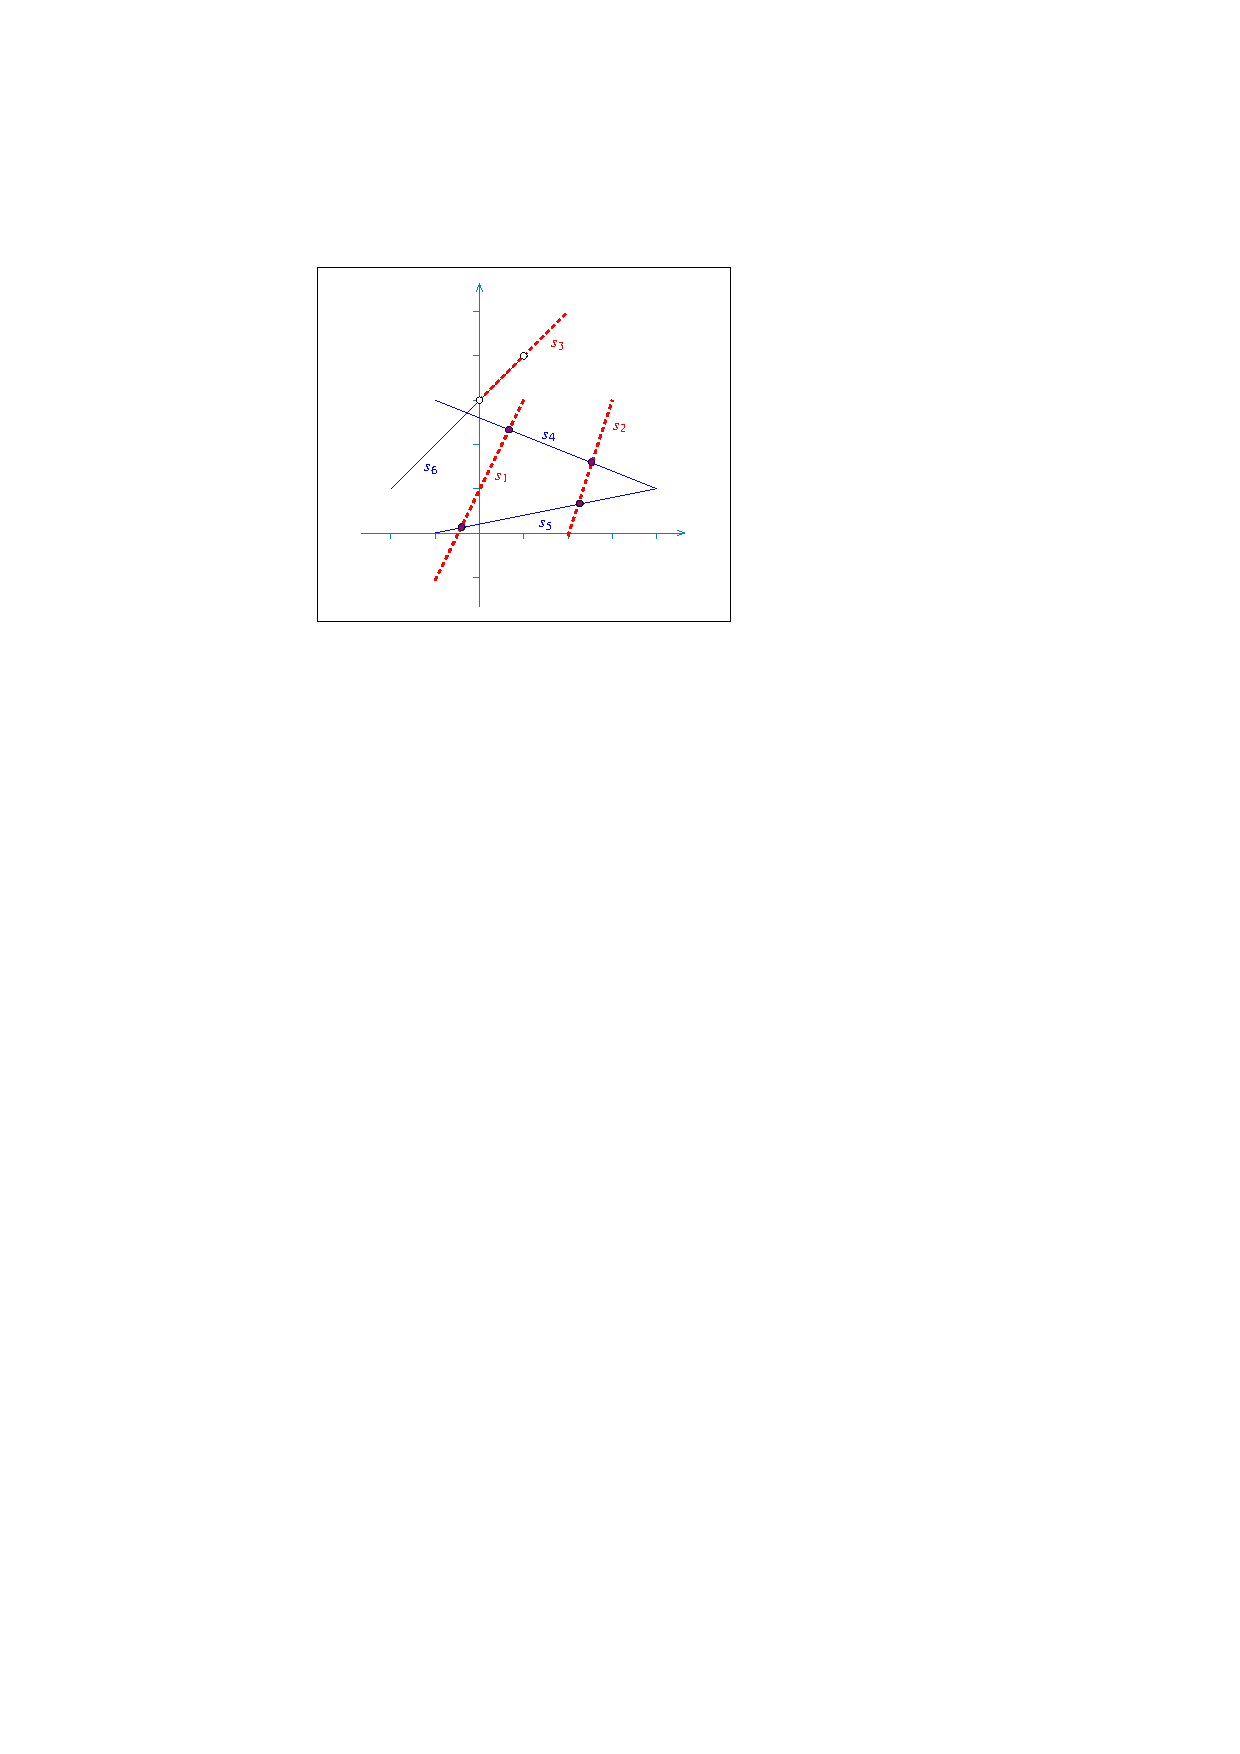
\includegraphics{Arrangement_on_surface_2/fig/ex_17}
  \end{center}
\end{ccTexOnly}
\begin{ccHtmlOnly}
  <p><center>
  <img src="./fig/ex_17.gif" border=0 alt="Example 17">
  </center>
\end{ccHtmlOnly}
\caption{An arrangement of six red and blue segments, as
constructed in \ccc{consolidated_curve_data.cpp}. Disks correspond to
red--blue intersection points, while circles mark the endpoints
of red--blue overlaps.\label{arr_fig:ex_17}}
\end{figure}

In the following example, we use \ccc{Arr_segment_traits_2} as our
base-traits class, attaching an additional {\em color} field to
the segments using the consolidated curve-data traits class. A
color may be either {\em blue} or {\em red}. Having constructed
the arrangement of colored segments, as depicted in
Figure~\ref{arr_fig:ex_17}, we detect the vertices that have incident 
edges mapped to both blue and red segments. Thus, they correspond
to red--blue intersection points. We also locate the edge that
corresponds to overlaps between red and blue line segments:

\ccIncludeExampleCode{Arrangement_on_surface_2/consolidated_curve_data.cpp}

\begin{figure}[t]
\begin{ccTexOnly}
  \begin{center}
  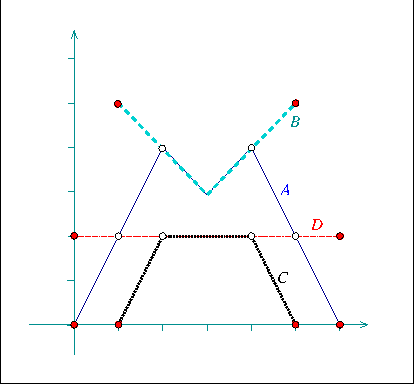
\includegraphics{Arrangement_on_surface_2/fig/ex_18}
  \end{center}
\end{ccTexOnly}
\begin{ccHtmlOnly}
  <p><center>
  <img src="./fig/ex_18.gif" border=0 alt="Example 18">
  </center>
\end{ccHtmlOnly}
\caption{An arrangement of four polylines, named A--D, as
constructed in \ccc{generic_curve_data.cpp}.\label{arr_fig:ex_18}}
\end{figure}

In the following example, we use \ccc{Arr_polyline_traits_2} as
our base-traits class, attaching an additional {\em name} field to
each polyline using the generic curve-data traits class. In case of
overlaps, we simply concatenate the names of the overlapping
polylines. Also notice how we replace the curve associated with
the edges that correspond to overlapping polylines with 
geometrically equivalent curves, but with a different data fields:

\ccIncludeExampleCode{Arrangement_on_surface_2/generic_curve_data.cpp}

The third example we give in this section is based on \ccc{dual_lines.cpp}
given in Section~\ref{arr_ssec:unb_global}. It constructs the arrangement
of the dual lines for a set of point given in an input file (by default we
use \ccc{coll_points.dat}, which contains $50$ points randomly selected
on the grid $[-100,100]\times[-100,100]$; the file contains two distinct
triplets of collinear points). Here we use the generic curve-data
decorator to attach the index of the primal point to each of the lines.
Doing so, we can go over the incident edges of each vertex whose degree is
greater than $4$ and report the subsets collinear points (if we have a vertex
of degree $d$, we actually need to go over $\frac{d}{2}$ edges, as each
incident line contributes exactly $2$ edges). Note that in this case the
dual line cannot overlap, so we use a dummy merge functor to instantiate
the curve-data traits:

\ccIncludeExampleCode{Arrangement_on_surface_2/dual_with_data.cpp}

\section{The Notification Mechanism}
\label{arr_sec:notif}
%===================================

For some applications it is essential to know exactly what
happens inside a specific arrangement-instance. For example, when
a new curve is inserted into an arrangement, it might be desired to keep
track of the faces that are split due to this insertion operation.
Other important examples are the point-location strategies that
require auxiliary data-structures (see Section~\ref{arr_ssec:pl}),
which must be notified on various local changes in the arrangement,
in order to keep their data structures up-to-date. The arrangement
package offers a mechanism that uses {\em observers} 
(see~\cite{cgal:ghjv-dpero-95}) that can be
attached to an arrangement instance and receive notifications
about the changes this arrangement goes through.

The \ccc{Arr_observer<Arrangement>} class-template is
parameterized with an arrangement class. It stores a pointer to an
arrangement object, and is capable of receiving notifications {\em
just before} a structural change occurs in the arrangement and
{\em immediately after} such a change takes place.
\ccc{Arr_observer} serves as a base class for other observer
classes and defines a set of virtual notification functions,
with default empty implementations.

The set of functions can be divided into three categories, as
follows:
\begin{enumerate}
\item Notifiers of changes that affect the entire topological structure
of the arrangement. This category consists of two pairs that
notify the observer of the following changes:
\begin{itemize}
\item The arrangement is cleared.
\item The arrangement is assigned with the contents of another
arrangement.
\end{itemize}
\item Pairs of notifiers of a local change that occurs in the
topological structure. Most notifier functions belong to this
category. The relevant local changes include:
\begin{itemize}
\item A new vertex is constructed and associated with a point.
\item An edge\footnote{The term ``edge'' refers here to a pair of twin
half-edges.} is constructed and associated with an $x$-monotone
curve.
\item An edge is split into two edges.
\item An existing face is split into two faces, as a consequence of the
insertion of a new edge.
\item A hole is created in the interior of a face.
\item Two holes are merged to form a single hole, as a consequence of the
insertion of a new edge.
\item A hole is moved from one face to another, as a consequence of
a face split.
\item Two edges are merged into one edge.
\item Two faces are merged into one face, as a consequence of the
removal of an edge that used to separate them.
\item One hole is split into two, as a consequence of the deletion of an 
edge that used to connect the two components.
\item A vertex is removed.
\item An edge is removed.
\item A hole is deleted from the interior of a face.
\end{itemize}
\item Notifiers about a change applied by a free (global) function.
This category consists of a single pair of notifiers, namely
\ccc{before_global_change()} and \ccc{after_global_change()}. Neither of
these functions is invoked by methods of the \ccc{Arrangement_2} class. 
Instead, they are called by the free functions themselves. It is implied 
that no point-location queries (or any other queries for that matter)
are issued between the calls to the notification functions above.
\end{enumerate}
See the Reference Manual for a detailed specification of the
\ccc{Arr_observer} class along with the exact prototypes of all
notification functions.

Each arrangement object stores a (possibly empty) list of pointers to
\ccc{Arr_observer} objects, and whenever one of the structural
changes listed in the first two categories above is about to take
place, the arrangement object performs a {\em forward} traversal
on this list and invokes the appropriate function of each
observer. After the change takes place the observer list is
traversed in a {\em backward} manner (from tail to head), and the
appropriate notification function is invoked for each observer.
This allows the nesting of observer objects.

Concrete arrangement-observer classes should inherit from
\ccc{Arr_observer}. When an observer is constructed, it is attached to
a valid arrangement supplied to the observed constructor, or alternatively 
the observer can be attached to the arrangement at a later time.
When this happens, the observer instance inserts itself into the
observer list of the associated arrangement and starts receiving
notifications whenever this arrangement changes thereafter. Naturally,
the observer object unregisters itself by removing itself from
this list just before it is destroyed.

The trapezoidal RIC and the landmark point-location strategies
both use observers to keep their auxiliary data structures
up-to-date. Besides them, users can define their own observer
classes, by inheriting from the base observer class and overriding
the relevant notification functions, as required by their
applications.

\begin{figure}[t]
\begin{ccTexOnly}
  \begin{center}
  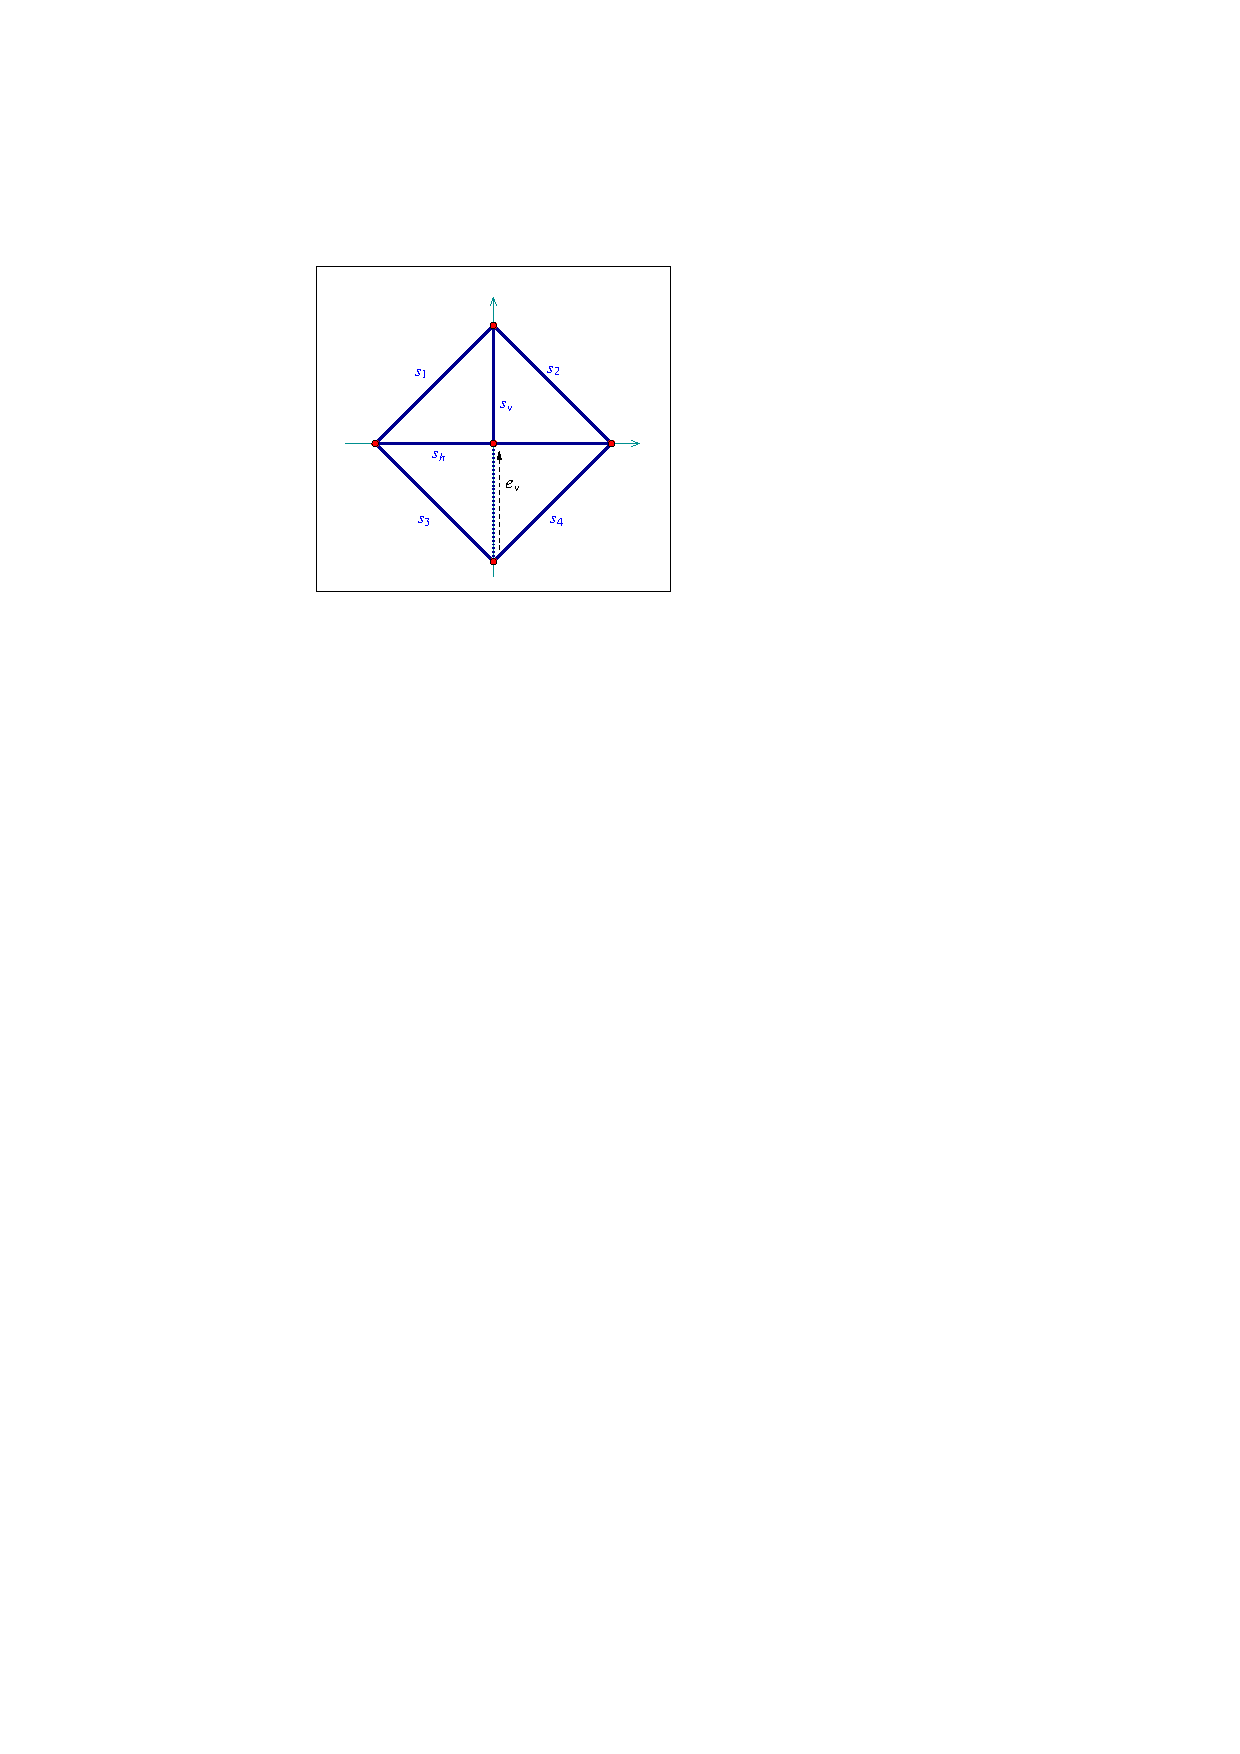
\includegraphics{Arrangement_2/fig/ex_19}
  \end{center}
\end{ccTexOnly}
\begin{ccHtmlOnly}
  <p><center>
  <img src="./fig/ex_19.gif" border=0 alt="Example 19">
  </center>
\end{ccHtmlOnly}
\caption{An arrangement of five line segments, as constructed in
\ccc{ex_observer.C}. The halfedge $e_v$ (dashed) is eventually
removed, so that the final arrangement consists of four faces (one
unbounded and three bounded ones).}
\label{arr_fig:ex_19}
\end{figure}

The following example shows how to define and use an observer
class. The observer in the example keeps track of the arrangement
faces, and prints a message whenever a face is split into two due
to the insertion of an edge, and whenever two faces merge into one
due to the removal of an edge. The layout of the arrangement is
depicted in Figure~\ref{arr_fig:ex_19}:

\ccIncludeExampleCode{../examples/Arrangement_2/ex_observer.C}

Observers are especially useful when the \dcel\ records are
extended and store additional data, as they help updating this
data on-line. See Section~\ref{arr_sec:ex_dcel} for more details
and examples.

\section{Extending the \dcel\label{arr_sec:ex_dcel}}
%============================

For many applications of the arrangement package it is necessary to
store additional information (perhaps of non-geometric nature) with
the arrangement cells. As vertices are associated with \ccc{Point_2}
objects and edges (halfedge pairs) are associated with
\ccc{X_monotone_curve_2} objects, both defined by the traits class,
it is possible to extend the traits-class type by using a traits-class
decorator, as explained in Section~\ref{arr_ssec:meta_tr}, which may
be a sufficient solution for some applications.
However, the \dcel\ faces are not associated with any geometric object, 
so it is impossible to extend them using a traits-class decorator. 
Extending the \dcel\ face records comes handy is such cases. As a matter
of fact, it is possible to conveniently extend all \dcel\ records
(namely vertices, halfedges and faces), which can also be advantageous
for some applications.

All examples presented so far use the default \ccc{Arr_default_dcel<Traits>}. 
This is done implicitly, as this class serves as a default parameter for 
the \ccc{Arrangement_2} template. The default \dcel\ class just associates 
points with vertices and $x$-monotone curves with halfedge, but nothing more. 
In this section we show how to use alternative \dcel\ types to extend the 
desired \dcel\ records.

\subsection{Extending the \dcel\ Faces\label{arr_ssec:ex_dcel_face}}
%--------------------------------------

The \ccc{Arr_face_extended_dcel<Traits, FaceData>} class-template
is used to associate auxiliary data field of type \ccc{FaceData} to
each face record in the \dcel.

When an \ccc{Arrangement_2} object is parameterized by this 
\dcel\ class, its nested \ccc{Face} type is extended with the access function
\ccc{data()} and with the modifier \ccc{set_data()}. Using these extra
functions it is straightforward to access and maintain the auxiliary
face-data field.

Note that the extra data fields must be maintained by the application
programmers. They may choose to construct their arrangement, and
only then go over the faces and attach the appropriate data fields to
the arrangement faces. However, in some cases the face data can only
be computed when the face is created (split from another face, or merged
with another face). In such cases one can use an arrangement observer
tailored for this task, which receives updates whenever a face is
modified and sets its data field accordingly.

\begin{figure}[t]
\begin{ccTexOnly}
  \begin{center}
  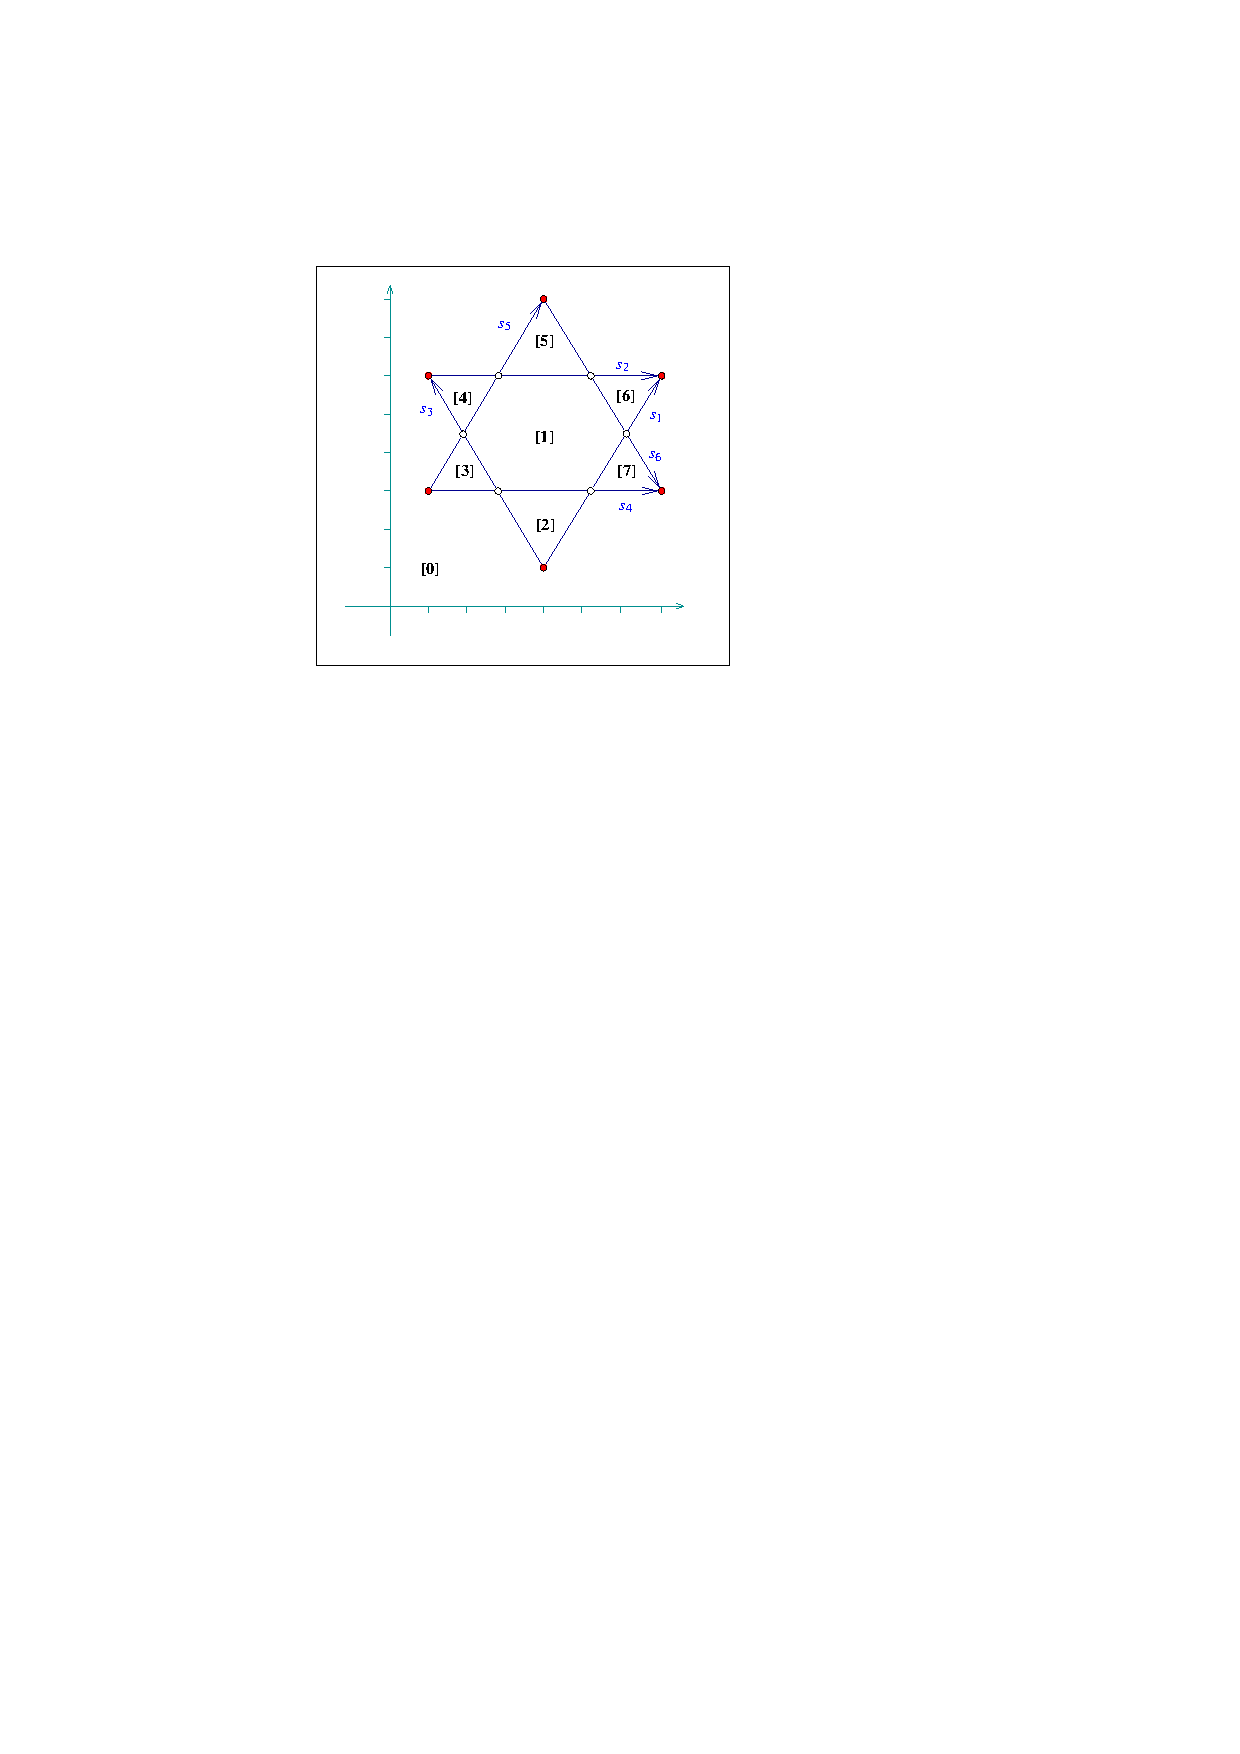
\includegraphics{Arrangement_2/fig/ex_20}
  \end{center}
\end{ccTexOnly}
\begin{ccHtmlOnly}
  <p><center>
  <img src="./fig/ex_20.gif" border=0 alt="Example 20">
  </center>
\end{ccHtmlOnly}
\caption{An arrangement of six line segments, as constructed in
\ccc{face_extension.cpp} and \ccc{dcel_extension.cpp}
(in \ccc{dcel_extension.cpp} we treat
the segments as directed, so they are drawn as arrows directed from the
source to the target). The indices associated with the halfedges in
\ccc{face_extension.cpp} are shown in brackets.\label{arr_fig:ex_20}}
\end{figure}

The next example constructs an arrangement that contains seven bounded 
faces induced by six line segments (see Figure~\ref{arr_fig:ex_20}). An 
observer gets notified each time a new face $f$ is created and it associates 
$f$ with a running index, (where the index of the unbounded face
is 0). As a result, the faces are numbered according to their creation
order, as one can easily verify by examining the insertion order of the
segments:\footnote{For simplicity, the particular observer used must be
attached to an empty arrangement. It is not difficult however to modify 
the program to handle the general case of attaching a similar observer
to a non-empty arrangement.}

\ccIncludeExampleCode{Arrangement_2/face_extension.cpp}

\subsection{Extending All \dcel\ Records\label{arr_ssec:ex_dcel_all}}
%----------------------------------------

The \ccc{Arr_extended_dcel<Traits, VertexData, HalfedgeData, FaceData>}
class-template is used to associate auxiliary data fields of
types \ccc{VertexData} \ccc{HalfedgeData}, and \ccc{FaceData} to
each \dcel\ vertex, halfedge, and face record types, respectively.

When an \ccc{Arrangement_2} object is injected with this
\dcel\ class, each one of its nested \ccc{Vertex}, \ccc{Halfedge} and
\ccc{Face} classes is extended by the access function \ccc{data()}
and by the modifier \ccc{set_data()}.

The next example shows how to use a \dcel\ with extended vertex,
halfedge, and face records. In this example each vertex is associated 
with a color, which may be blue, red, or white, depending on whether the
vertex is isolated, represents a segment endpoint, or whether it
represents an intersection point. Each halfedge is associated with
Boolean flag indicating whether its direction is the same as the
direction of its associated segment (in this example segments are
treated as directed objects). Each face is also extended to store the
size of its outer boundary.

The constructed arrangement, depicted in Figure~\ref{arr_fig:ex_20}, is 
similar to the arrangement constructed in the previous example. 
Note that all auxiliary data fields are set during the construction phase.
Also note that the data fields are properly maintained when the arrangement
is copied to another arrangement instance:
 
\ccIncludeExampleCode{Arrangement_2/dcel_extension.cpp}

\begin{ccAdvanced}
The various \dcel\ classes presented in this section are perfectly
sufficient for most applications based on the arrangement package.
However, users may also use their own implementation of a \dcel\ class
to instantiate the \ccc{Arrangement_2} class-template, in case they need
special functionality from their \dcel. Such a class must be a model of the
concept \ccc{ArrangementDcel}, whose exact specification is listed in the
Reference Manual.
\end{ccAdvanced}

\ccRefPageBegin

\begin{ccRefFunction}{overlay}

\ccDefinition

The function \ccRefName{} computes the overlay of two input arrangement
objects, and returns the overlaid arrangement. All three arrangements
can be instantiated with different geometric traits classes and different
\dcel{} (encapsulated in the various topology-traits classes) classes.
The geometry traits of the resulting arrangement is used to construct the
resulting arrangement. This means that all the types (e.g.,
\ccc{Traits::Point_2}, \ccc{Traits::Curve_2}, and \ccc{Traits::Point_2})
of both input arrangements have to be convertible to the types in the
resulting arrangement. A given overlay-traits object is used to properly
construct the overlaid \dcel{} that represents the resulting arrangement.

%%%%

\ccInclude{CGAL/Arr_overlay_2.h}

\ccGlobalFunction{template <class GeomTraitsA, class GeomTraitsB,
                            class GeomTraitsRes, class TopTraitsA,
                            class TopTraitsB, class TopTraitsRes,
                            class OverlayTraits>
  void overlay (const Arrangement_2<GeomTraitsA, TopTraitsA>& arr1,
                const Arrangement_2<GeomTraitsB, TopTraitsB>& arr2,
                Arrangement_2<GeomTraitsRes, TopTraitsRes>& arr_res,
                OverlayTraits& ovl_tr);}
Computes the overlay of two arrangements \ccc{arr1} and \ccc{arr2}, and sets
the output arrangement \ccc{res} to represent the overlaid arrangement.
\ccPrecond{\ccc{res} does not refer to either \ccc{arr1} or \ccc{arr2}
(that is, ``self overlay'' is not supported).}

\ccGlobalFunction{template <class GeomTraitsA, class GeomTraitsB,
                            class GeomTraitsRes, class TopTraitsA,
                            class TopTraitsB, class TopTraitsRes>
  void overlay (const Arrangement_2<GeomTraitsA, TopTraitsA>& arr1,
                const Arrangement_2<GeomTraitsB, TopTraitsB>& arr2,
                Arrangement_2<GeomTraitsRes, TopTraitsRes>& arr_res);}
Computes the (simple) overlay of two arrangements \ccc{arr1} and \ccc{arr2},
and sets the output arrangement \ccc{res} to represent the overlaid
arrangement. It employs the default overlay-traits, which practically does
nothing.
\ccPrecond{\ccc{res} does not refer to either \ccc{arr1} or \ccc{arr2}
(that is, ``self overlay'' is not supported).}

%%%%

\ccThree{Orientation~~}{}{\hspace*{8.5cm}}

\ccInclude{CGAL/Arrangement_with_history_2.h}

\ccGlobalFunction{template<typename Traits, typename Dcel1, typename Dcel2,
                           typename ResDcel, typename OverlayTraits>
           void overlay (const Arrangement_with_history_2<Traits,Dcel1>& arr1,
                         const Arrangement_with_history_2<Traits,Dcel2>& arr2,
                         Arrangement_with_history_2<Traits,ResDcel>& res,
                         OverlayTraits& ovl_tr);}
Computes the overlay of two arrangements with history \ccc{arr1} and
\ccc{arr2}, and sets the output arrangement with history \ccc{res} to
represent the overlaid arrangement. The function also constructs a
consolidated set of curves that induce \ccc{res}.
\ccPrecond{\ccc{res} does not refer to either \ccc{arr1} or \ccc{arr2}
(that is, ``self overlay'' is not supported).}

\ccGlobalFunction{template<typename Traits, typename Dcel1, typename Dcel2,
                           typename ResDcel>
           void overlay (const Arrangement_with_history_2<Traits,Dcel1>& arr1,
                         const Arrangement_with_history_2<Traits,Dcel2>& arr2,
                         Arrangement_with_history_2<Traits,ResDcel>& res);}
Computes the (simple) overlay of two arrangements with history \ccc{arr1}
and \ccc{arr2}, and sets the output arrangement with history \ccc{res} to
represent the overlaid arrangement. The function also constructs a
consolidated set of curves that induce \ccc{res}. It employs the default
overlay-traits, which practically does nothing.
\ccPrecond{\ccc{res} does not refer to either \ccc{arr1} or \ccc{arr2}
(that is, ``self overlay'' is not supported).}

\ccRequirements
\begin{itemize}
\item The overlay-traits object \ccc{ovl_tr} must model the \ccc{OverlayTraits}
  concept, which is able to construct records of the \ccc{ResDcel} class on
  the basis of the \ccc{Dcel1} and \ccc{Dcel2} records that induce them.
\end{itemize}

\ccSeeAlso
  \ccc{OverlayTraits}\lcTex{(\ccRefPage{OverlayTraits})}

\end{ccRefFunction}

\ccRefPageEnd

\section{Storing the Curve History\label{arr_sec:arr_with_hist}}
%==================================

As stated at the beginning of this chapter (Section~\ref{arr_sec:intro}), 
when one constructs an arrangement induced by a set $\calC$ of arbitrary 
planar curves, she or he constructs a collection $\calC''$ of $x$-monotone 
subcurves of $\calC$ that are pairwise disjoint in their interior, and these 
subcurves are associated with the arrangement edges (more precisely, with the 
\dcel\ halfedges). Doing so, the connection between the originating input 
curves and the arrangement edges is lost. This loss might be acceptable for 
some applications. However, in many practical cases it is important to 
determine the input curves that give rise to the final subcurves.

The \ccc{Arrangement_with_history_2<Traits,Dcel>} class-template extends
the \ccc{Arrangement_2} class by keeping an additional container of input
curves representing $\calC$, and by maintaining a cross-mapping between these
curves and the arrangement edges they induce. The traits class that is
used for instantiating the template should be a model of the
\ccc{ArrangementTraits_2} concept (see Section~\ref{arr_sssec:insert_gen}).
That is, it should define the \ccc{Curve_2} type (and not just the
\ccc{X_monotone_curve_2} type). The \ccc{Dcel} parameter should model the 
\ccc{ArrangementDcel} concept. Users can use the default \dcel\ class or 
an extended \dcel\ class according to their needs.

\subsection{Traversing an Arrangement with History\label{arr_ssec:arrwh_traverse}}
%--------------------------------------------------

The \ccc{Arrangement_with_history_2} class extends the \ccc{Arrangement_2}
class, thus all the iterator and circulator types that are defined by the
arrangement class are also available in \ccc{Arrangement_with_history_2}.
The reader is referred to Section~\ref{arr_ssec:traverse} for a comprehensive
review of these functions.

As mentioned above, the \ccc{Arrangement_with_history_2} class maintains
a container of input curves, which can be accessed using curve handles.
The member function \ccc{number_of_curves()} returns the number of input 
curves stored in the container, while \ccc{curves_begin()} and 
\ccc{curves_end()} return \ccc{Arrangement_with_history_2::Curve_iterator}
objects that define the  valid range of curves that induce the arrangement.
The value type of this iterator is \ccc{Curve_2}. Moreover, the curve-iterator
type is equivalent to  \ccc{Arrangement_with_history_2::Curve_handle}, which
is used for accessing the stored curves. Conveniently, the corresponding
constant-iterator and constant-handle types are also defined.

As mentioned in the previous paragraph, a \ccc{Curve_handle} object \ccc{ch} 
serves as a pointer to a curve stored in an arrangement-with-history instance 
\ccc{arr}. Using this handle, it is possible to obtain the number of 
arrangement edges this curve induces by calling 
\ccc{arr.number_of_induced_edges(ch)}. The functions 
\ccc{arr.induced_edges_begin(ch)} and
\ccc{arr.induced_edges_end(ch)} return iterators of type
\ccc{Arrangement_with_history_2::Induced_edges_iterator} that define the
valid range of edges induced by \ccc{ch}. The value type of these iterators
is \ccc{Halfedge_handle}. It is thus possible to traverse all arrangement
edges induced by an input curve.

It is also important to be able to perform the inverse mapping. Given an
arrangement edge, we would like to be able to determine which input curve
induces it. In case the edge represents an overlap of several curves, we
should be able to trace all input curves that overlap over this edge.
The \ccc{Arrangement_with_history_2} class is extended by several member
functions that enable such an inverse mapping. Given a halfedge handle \ccc{e}
in an arrangement with history \ccc{arr}, then 
\ccc{arr.number_of_originating_curves(e)} returns the number of curves that
induce the edge (which should be 1 in non-degenerate cases, and 2 or more
in case of overlaps), while \ccc{arr.originating_curves_begin(e)} and 
\ccc{arr.originating_curves_end(e)} return 
\ccc{Arrangement_with_history_2::Originating_curve_iterator} objects that
define the range of curves that induce \ccc{e}. The value type of these
iterator is \ccc{Curve_2}.

It is possible to overlay two \ccc{Arrangement_with_history_2} instances 
instantiated by the same traits class. In this case, the resulting 
arrangement will store a consolidated container of input curves, and 
automatically preserve the cross-mapping between the arrangement edges 
and the consolidated curve set. Users can employ an overlay-traits class
to maintain any type of auxiliary data stored with the \dcel\ features
(see Section~\ref{arr_sec:overlay}).

\subsection{Modifying an Arrangement with History\label{arr_ssec:modif_traverse}}
%-------------------------------------------------

As the \ccc{Arrangement_with_history_2} class extends the \ccc{Arrangement_2}
class, it inherits the fundamental modification operations, such as 
\ccc{assign()} and \ccc{clear()}, from it. The vertex-manipulation functions
are also inherited and supported (see Sections~\ref{arr_sssec:mf_iso_verts}
and~\ref{arr_sssec:insert_point} for the details). However, there are some 
fundamental differences between the interfaces of the two classes, which we
highlight in this subsection.

The most significant difference between the arrangement-with-history class
and the basic arrangement class is the way they handle their input curves.
\ccc{Arrangement_with_history_2} always stores the \ccc{Curve_2} objects
that induce it, thus it is impossible to insert $x$-monotone curves into
an arrangement with history. The free \ccc{insert_non_intersecting_curve()}
and \ccc{insert_x_monotone_curve()} (as well as their aggregated versions)
are therefore not available for arrangement-with-history instances
and only the free \ccc{insert_curve()} and \ccc{insert_curves()} functions
(the incremental insertion function and the aggregated insertion function)
are supported --- see also Section~\ref{arr_sssec:insert_gen}. Notice however
that while the incremental insertion function \ccc{insert_curve(arr,c)} for
an \ccc{Arrangement_2} object \ccc{arr} does not have a return value,
the corresponding arrangement-with-history function returns a
\ccc{Curve_handle} to the inserted curve.

As we are able to keep track of all edges induced by an input curve, we also
provide a free function that removes a curve from an arrangement. By calling
\ccc{remove(arr,ch)}, where \ccc{ch} is a valid curve handle, the given curve
is deleted from the curve container, and all edges induced solely by
this curve (i.e., excluding overlapping edges) are removed from the 
arrangement. The function returns the number of edges that have been removed.

In some cases, users may need to operate directly on the arrangement edges.
We first mention that the specialized insertion functions (see 
Section~\ref{arr_sssec:mf_insert_cv}) are not supported, as they accept
$x$-monotone curves. Insertion can only be performed via the free 
insertion-functions. The other edge-manipulation functions 
(see Section~\ref{arr_sssec:mf_halfedges}) are however available, but have 
a different interface that does not use $x$-monotone curves:
\begin{itemize}
\item Invoking \ccc{split_edge(e,p)} splits the edge \ccc{e} at a given point
\ccc{p} that lies in its interior.
\item Invoking \ccc{merge_edge(e1,e2)} merges the two given edges. There is
a precondition that \ccc{e1} and \ccc{e2} shared a common end-vertex of degree
2, and that the $x$-monotone subcurves associated with these edges are
mergeable.
\item It is possible to remove an edge by simply invoking
\ccc{remove_edge(e)}.
\end{itemize}
In all cases, the maintenance of cross-pointers for the appropriate input
curves will be done automatically.

It should be noted that it is possible to attach observers to an 
arrangement-with-history instance in order to get detailed notifications of
the changes the arrangements undergoes (see Section~\ref{arr_sec:notif} for
the details).

\subsection{Examples\label{arr_ssec:arr_hist_ex}}
%---------------------------

\begin{figure}[t]
\begin{ccTexOnly}
  \begin{center}
  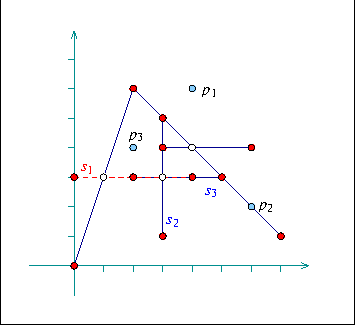
\includegraphics{Arrangement_2/fig/ex_24}
  \end{center}
\end{ccTexOnly}
\begin{ccHtmlOnly}
  <p><center>
  <img src="./fig/ex_24.gif" border=0 alt="Example 24">
  </center>
\end{ccHtmlOnly}
\caption{An arrangement with history as constructed in
\ccc{ex_curve_history.cpp}. 
Note that $s_1$ and $s_3$ overlap over two edges. The point-location query
points are drawn as lightly shaded dots.\label{arr_fig:ex_24}}
\end{figure}

In the following example we construct a simple arrangement of six line
segments, as depicted in Figure~\ref{arr_fig:ex_24}, while maintaining 
the curve history. The example demonstrates the usage of the special
traversal functions. It also shows how to issue point-location queries
on the resulting arrangement, using the auxiliary function 
\ccc{point_location_query()} defined in the header file 
\ccc{point_location_utils.h} (see also Section~\ref{arr_ssec:pl}).

\ccIncludeExampleCode{../examples/Arrangement_2/ex_curve_history.cpp}

\begin{figure}[t]
\begin{ccTexOnly}
  \begin{center}
  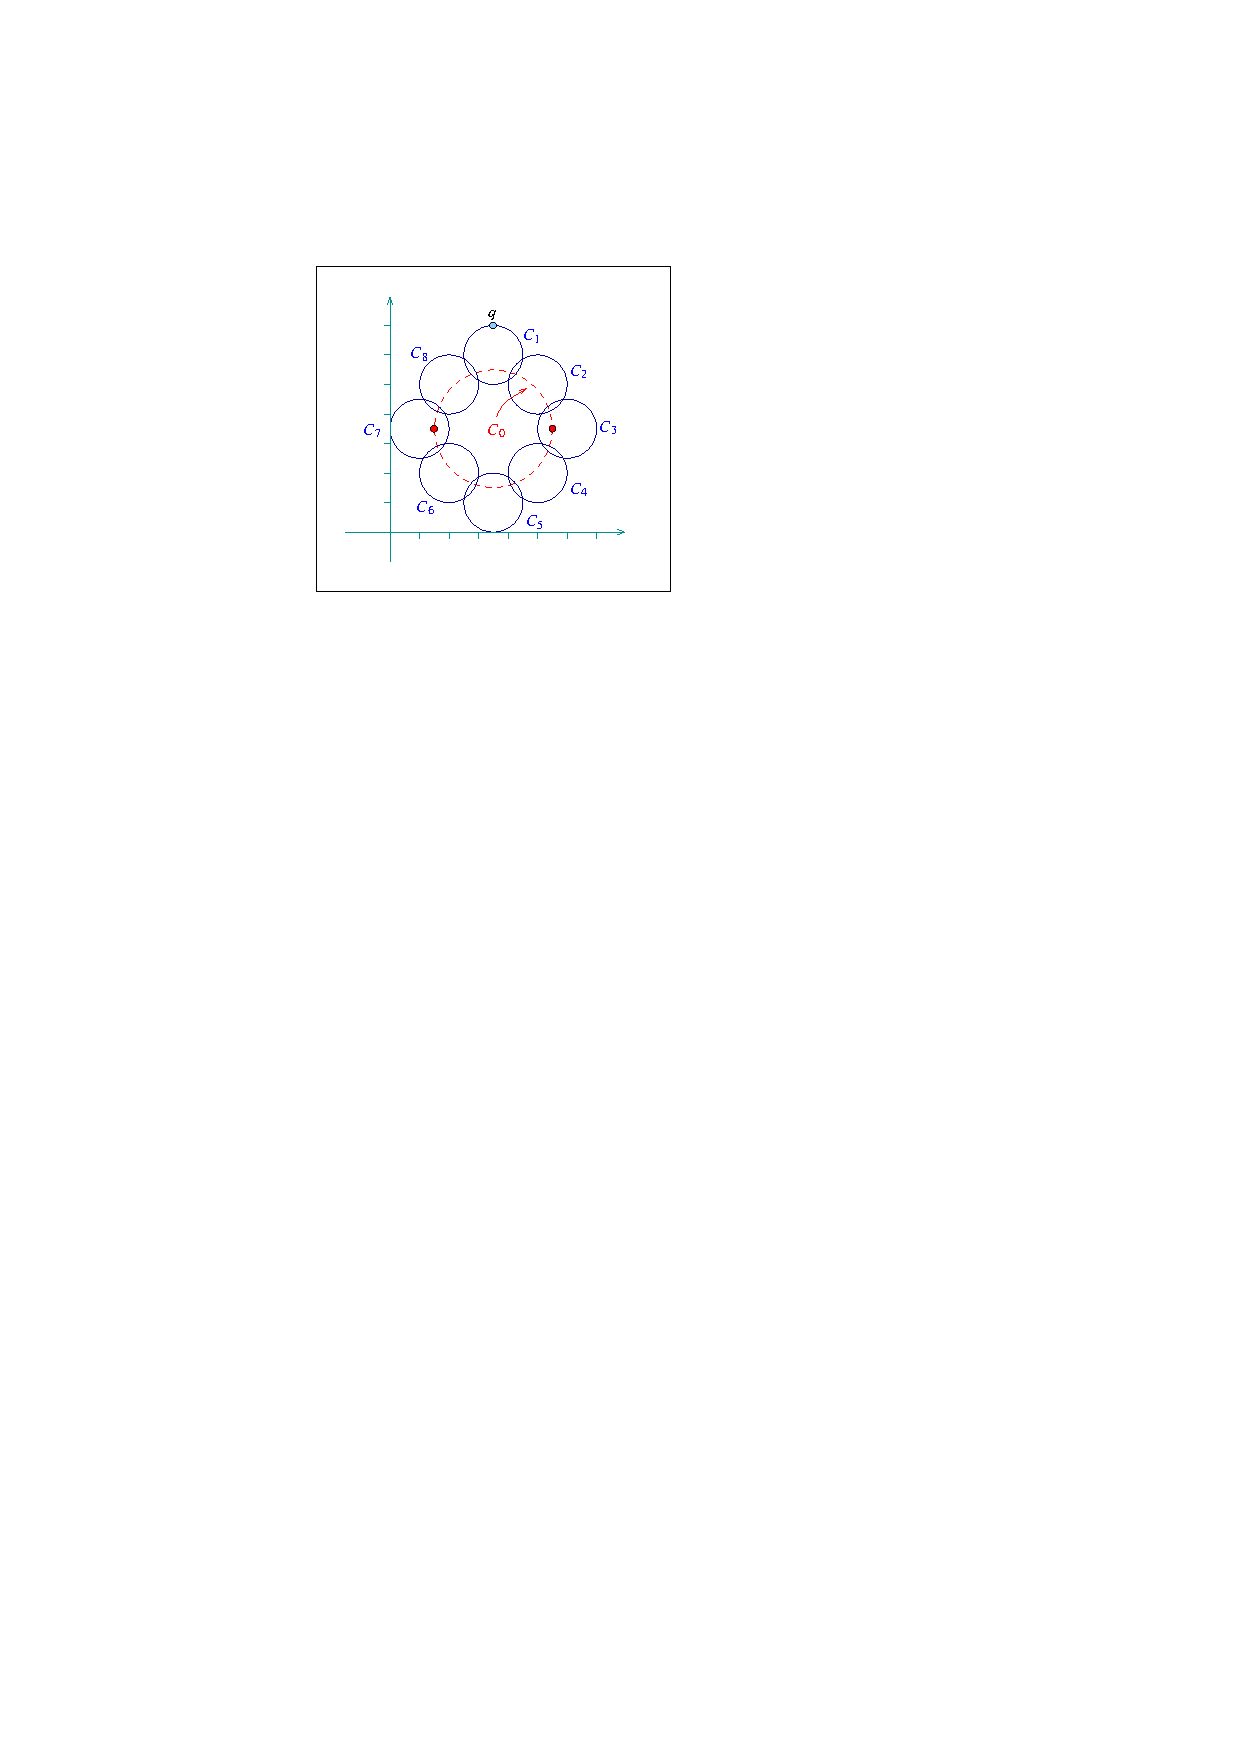
\includegraphics{Arrangement_2/fig/ex_25}
  \end{center}
\end{ccTexOnly}
\begin{ccHtmlOnly}
  <p><center>
  <img src="./fig/ex_25.gif" border=0 alt="Example 25">
  </center>
\end{ccHtmlOnly}
\caption{An arrangement with history of nine circle as constructed in 
\ccc{ex_edge_manipulation_curve_history.cpp}. Note the vertical tangency points
of $C_0$, marked as dark dots, which subdivide this circle into an upper half
and a lower half, each consists of 9 edges. The large circle $C_0$ is
eventually removed from the arrangement, with all 18 edges it
induces.\label{arr_fig:ex_25}}
\end{figure}

The following example demonstrates the usage of the free \ccc{remove()}
function. We construct an arrangement of nine circles, while keeping a handle
to each inserted circle. We then remove the large circle $C_0$, which induces
$18$ edges, as depicted in Figure~\ref{arr_fig:ex_25}. The example also shows
how to use the \ccc{split_edge()} and \ccc{merge_edge()} functions when
operating on an arrangement-with-history instance:

\ccIncludeExampleCode{../examples/Arrangement_2/ex_edge_manipulation_curve_history.cpp}

\section{Input/Output Streams\label{arr_sec:io}}
%===============================

In some cases, one would like to save an arrangement object constructed
by some application, so that later on it can be restored. In other cases 
one would like to create a nice drawings that represent an arrangement 
constructed by some application. These drawings can hard printed or
displayed on a computer screen.

\subsection{Input/Output Stream}\label{arr_ssec:io_stream}
%--------------------------------------------
Consider an arrangement that represents a very complicated geographical 
map, and assume that there are various applications that need to answer 
point-location queries on this map. Naturally, you can store the set of 
curves that induces the arrangement, but this implies that you would need 
to construct the arrangement from scratch each time you need to reuse it.
A more efficient solution is to write the arrangement to a file in a format 
that other applications can read.

This package provides an {\em inserter} (the \ccc{<<} operator) and an 
{\em extractor} (the \ccc{>>} operator) for the 
\ccc{Arrangement_2<Traits,Dcel>} class, such that an arrangement object 
can be inserted into an output stream or read from an input stream. The 
arrangement is written using a simple predefined ASCII format that encodes 
the arrangement topology, as well as all geometric entities associated with 
vertices and edges.

The ability to use the input/output operators, requires that the 
\ccc{Point_2} type and the \ccc{X_monotone_curve_2} type defined by the 
traits class both support the \ccc{<<} and \ccc{>>} operators. The 
\ccc{Arr_conic_traits_2} class (see Section~\ref{arr_ssec:tr_conic}), the 
\ccc{Arr_rational_arc_traits_2} class (see Section~\ref{arr_ssec:tr_ratfunc}),
and the \ccc{Arr_linear_traits_2} class (see Section~\ref{arr_ssec:tr_segs})
currently do not provide these operators for the geometric types they define. 
Thus, only arrangements of line segments or of polylines can be written or 
read.

The following example constructs the arrangement depicted in 
Figure~\ref{arr_fig:ex_5} and writes it to an output file. It also
demonstrates how to re-read the arrangement from a file:

\ccIncludeExampleCode{Arrangement_2/ex_io.cpp}

\begin{ccAdvanced}
\subsection{Arrangements with Auxiliary Data\label{arr_ssec:arr_io_aux_data}}
%--------------------------------------------

The inserter and extractor both ignore any auxiliary data stored with
the arrangement features. Thus, they are ideal for arrangements
instantiated using the \ccc{Arr_default_dcel} class.
However, as explained in Section~\ref{arr_sec:ex_dcel}, one can easily
extend the arrangement faces by using the \ccc{Arr_face_extended_dcel}
template, or extend all \dcel\ records by using the \ccc{Arr_extended_dcel}
template. In such cases, it might be crucial that the auxiliary data fields
are written to the file and read from there.

The arrangement package includes the free functions
\ccc{write(arr, os, formatter)}, which writes the arrangement \ccc{arr}
to an output stream \ccc{os}, and \ccc{read(arr, os, formatter)}, which
reads the arrangement \ccc{arr} from an input stream \ccc{is}. Both
operations are performed using a \ccc{formatter} object, which defines
the I/O format. The package contains three formatter classes:
\begin{itemize}
\item \ccc{Arr_text_formatter<Arrangement>} defines a simple textual
I/O format for the arrangement topology and geometry, disregarding any
auxiliary data that may be associated with the arrangement features.
This is the default formatter used by the arrangement inserter and the
arrangement extractor, as defined above.
%
\item \ccc{Arr_face_extended_text_formatter<Arrangement>} operates on
arrangements whose \dcel\ representation is based on the
\ccc{Arr_face_extended_dcel<Traits,FaceData>} class (see
Section~\ref{arr_ssec:ex_dcel_face}). It supports reading and writing
the auxiliary data objects stored with the arrangement faces provided
that the \ccc{FaceData} class supports an inserter and an extractor.
%
\item \ccc{Arr_extended_dcel_text_formatter<Arrangement>} operates on
arrangements whose \dcel\ representation is based on the
\ccc{Arr_extended_dcel<Traits,VertexData,HalfedgeData,FaceData>} class
(see Section~\ref{arr_ssec:ex_dcel_all}). It supports reading and writing
the auxiliary data objects stored with the arrangement vertices, edges
and faces, provided that the \ccc{VertexData}, \ccc{HalfedgeData} and
\ccc{FaceData} classed all have inserters and extractors.
\end{itemize}

The following example constructs the same arrangement as the
example \ccc{ex_dcel_extension} does
(see Section~\ref{arr_ssec:ex_dcel_all}), depicted in
Figure~\ref{arr_fig:ex_20}, and writes it to an output file. It also
demonstrates how to re-read the arrangement from a file:

\ccIncludeExampleCode{Arrangement_2/ex_dcel_extension_io.cpp}

You may develop your own own formatter classes --- models of the
\ccc{ArrangementInputFormatter} and \ccc{ArrangementOutputFormatter}
concepts, as defined in the Reference Manual.
Doing so, you can define other I/O formats, such as an XML-based
format or a binary format.
\end{ccAdvanced}

\subsection{Arrangements with Curve History\label{arr_ssec:arr_io_hist}}
%-------------------------------------------

Section~\ref{arr_sec:arr_with_hist} introduces the
\ccc{Arrangement_with_history_2<Traits,Dcel>} class, which saves the
set of curves inducing an arrangement and maintains the relations between
these curves and the edges they induce. Naturally, when reading or writing 
an arrangement-with-history instance we would like this information to be
saved to the output stream or restored from the input stream alongside
with the basic arrangement structure.

The arrangement package supplies an inserter and an extractor for the
\ccc{Arrangement_with_history_2<Traits,Dcel>} class. The arrangement is
represented using a simple predefined ASCII format. An object of the
\ccc{Arrangement_with_history_2<Traits,Dcel>} type can be saved and 
restored, as long as the \ccc{Curve_2} type defined by the traits 
class --- as well as the \ccc{Point_2} type and the \ccc{X_monotone_curve_2} 
types --- support the \ccc{<<} and\ccc{>>} operators.

The following example constructs the same arrangement as example
\ccc{ex_curve_history} does
(see Section~\ref{arr_ssec:arr_hist_ex}), depicted in 
Figure~\ref{arr_fig:ex_24}, and writes it to an output file. It also
demonstrates how to re-read the arrangement-with-history from a file:

\ccIncludeExampleCode{Arrangement_2/ex_io_curve_history.cpp}

\begin{ccAdvanced}
The arrangement package also includes the free functions
\ccc{write(arr, os, formatter)} and \ccc{read(arr, os, formatter)} that
operate on a given arrangement-with-history instance \ccc{arr}.
Both functions are parameterized by a \ccc{formatter} object, which define
the I/O format. The package contains a template called,
\ccc{Arr_with_hist_text_formatter<ArranagmentFormatter>}, which extends
an arrangement formatter class (see Section~\ref{arr_ssec:arr_io_aux_data})
and defines a simple textual input/output format.
\end{ccAdvanced}

\subsection{Output Postscript Stream}\label{arr_ssec:ps_stream}
%--------------------------------------------
You can create nice drawings of arrangements in Postscript format, which
you can insert into your publications, using the utility class 
\ccc{Arr_postscript_file_stream}. This class is derived from the 
\ccc{Postscript_file_stream} utility class, which in turn is derived from
the \leda\ class \ccc{ps_file}. The \ccc{Arr_postscript_file_stream}
class allows you to specify the color of points and curves separately
in addition to the functionality of the based class.

\section{Adapting to {\sc Boost} Graphs\label{arr_sec:bgl}}
%=======================================

\boost\footnote{See also {\sc Boost}'s homepage at: {\tt www.boost.org}.}
is a collection of portable \CC\
libraries that extend the Standard Template Library ({\sc Stl}). The \boost\
Graph Library (\bgl), which one of the libraries in the collection, offers an
extensive set of generic graph algorithms parameterized through templates.
As our arrangements are embedded as planar graphs, it is only 
natural to extend the underlying data structure with the interface that the 
\bgl\ expects, and gain the ability to perform the operations that the \bgl\
supports, such as shortest-path computation. This section describes how apply
the graph algorithms implemented in the \bgl\ to \ccc{Arrangement_2} instances.

An instance of \ccc{Arrangement_2} is adapted to a \boost\ graph through the
provision of a set of free functions that operate on the arrangement features
and conform with the relevant BGL concepts. Besides the straightforward 
adaptation, which associates a vertex with each \dcel\ vertex and an edge 
with each \dcel\ halfedge, the package also offer a {\em dual} adaptor, which 
associates a graph vertex with each \dcel\ face, such that two vertices are 
connected, iff there is a \dcel\ halfedge that connects the two corresponding
faces. 

\subsection{The Primal Arrangement Representation\label{arr_ssec:bgl_primal}}
%-------------------------------------------------

Arrangement instances are adapted to \boost\ graphs by specializing the
\ccc{boost:graph_traits} template for \ccc{Arrangement_2} instances. The
graph-traits states the graph concepts that the arrangement class models
(see below) and defines the types required by these concepts.

In this specialization the \ccc{Arrangement_2} vertices correspond to the
graph vertices, where two vertices are adjacent if there is at least one
halfedge connecting them. More precisely, \ccc{Arrangement_2::Vertex_handle}
is the graph-vertex type, while \ccc{Arrangement_2::Halfedge_handle} is the
graph-edge type. As halfedges are directed, we consider the graph to be
directed as well. Moreover, as several interior-disjoint $x$-monotone curves
(say circular arcs) may share two common endpoints, inducing an arrangement
with two vertices that are connected with several edges, we allow parallel
edges in our \boost\ graph.

Given an \ccc{Arrangement_2} instance, we can efficiently traverse its
vertices and halfedges. Thus, the arrangement graph is a model of the concepts
\ccc{VertexListGraph} and \ccc{EdgeListGraph} introduced by the \bgl.
At the same time, we use an iterator adapter of the circulator over the
halfedges incident to a vertex (\ccc{Halfedge_around_vertex_circulator} --- see
Section~\ref{arr_sssec:tr_vertex}), so it is possible to go over the ingoing
and outgoing edges of a vertex in linear time. Thus, our arrangement graph
is a model of the concept \ccc{BidirectionalGraph} (this concept refines
\ccc{IncidenceGraph}, which requires only the traversal of outgoing edges).

It is important to notice that the vertex descriptors we use are
\ccc{Vertex_handle} objects and {\em not} vertex indices. However, in order
to gain more efficiency in most \bgl\ algorithm, it is better to have them
indexed $0, 1, \ldots, (n-1)$, where $n$ is the number of vertices. We
therefore introduce the \ccc{Arr_vertex_index_map<Arrangement>} class-template,
which maintains a mapping of vertex handles to indices, as required by the
\bgl. An instance of this class must be attached to a valid arrangement
vertex when it is created. It uses the notification mechanism (see
Section~\ref{arr_sec:notif}) to automatically maintain the mapping of vertices
to indices, even when new vertices are inserted into the arrangement or
existing vertices are removed.

In most algorithm provided by the \bgl, the output is given by
{\em property maps}, such that each map entry corresponds to a vertex.
For example, when we compute the shortest paths from a given source vertex
$s$ to all other vertices we can obtain a map of distances and a map of
predecessors --- namely for each $v$ vertex we have its distance from $s$
and a descriptor of the vertex that precedes $v$ in the shortest path from $s$.
If the vertex descriptors are simply indices, one can use vectors to
efficiently represent the property maps. As this is not the case with the
arrangement graph, we offer the \ccc{Arr_vertex_property_map<Arrangement,Type>}
template allows for an efficient mapping of \ccc{Vertex_handle} objects to
properties of type \ccc{Type}. Note however that unlike the
\ccc{Arr_vertex_index_map} class, the vertex property-map class is not
kept synchronized with the number of vertices in the arrangement, so it
should not be reused in calls to \bgl\ functions in case the arrangement
is modified in between these calls.

\begin{figure}[t]
\begin{ccTexOnly}
  \begin{center}
  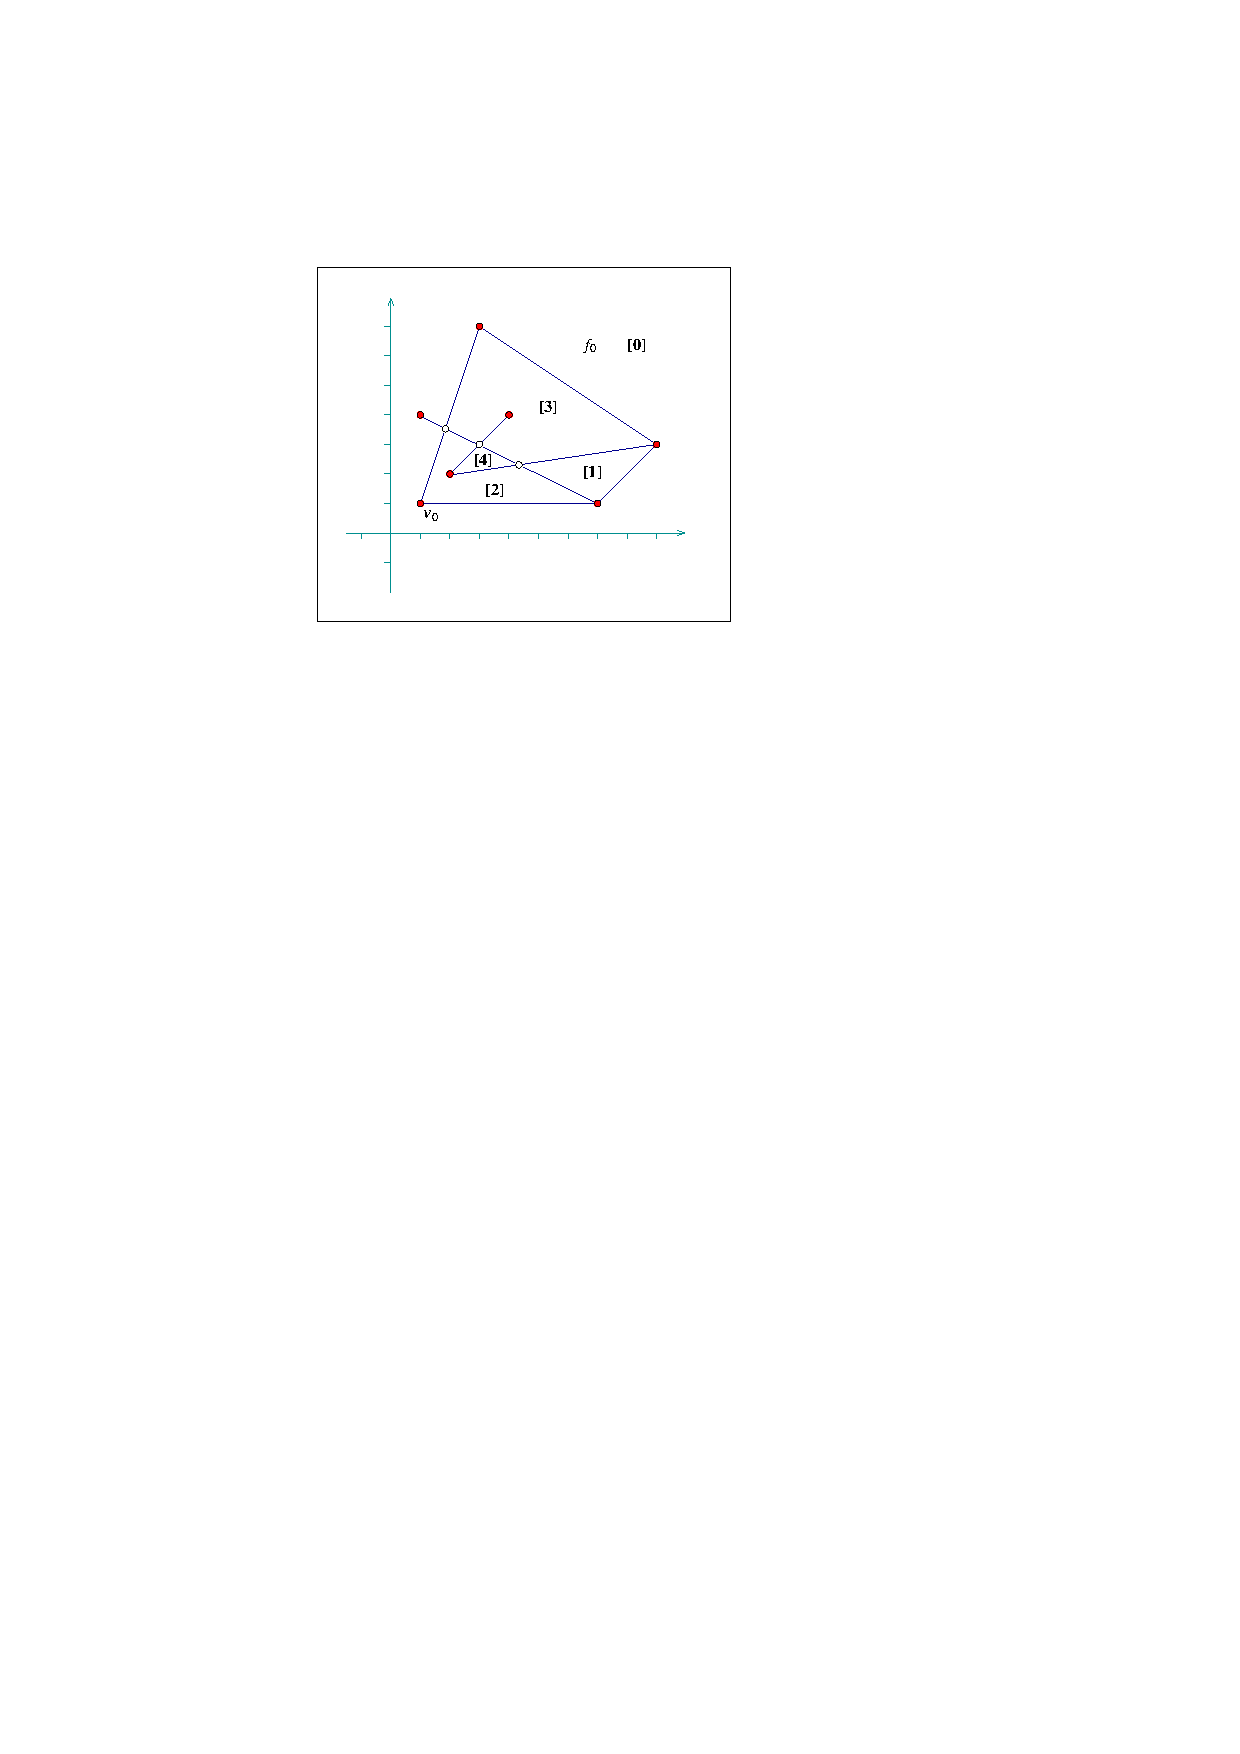
\includegraphics{Arrangement_2/fig/ex_bgl}
  \end{center}
\end{ccTexOnly}
\begin{ccHtmlOnly}
  <p><center>
  <img src="./fig/ex_bgl.gif" border=0 alt="Example BGL">
  </center>
\end{ccHtmlOnly}
\caption{An arrangement of 7 line segments, as constructed by
\ccc{ex_bgl_primal_adapter.C} and \ccc{ex_bgl_dual_adapter.C}.
The breadth-first visit times for the arrangement faces, starting
from the unbounded face $f_0$, are shown is brackets.}
\label{arr_fig:ex_bgl}
\end{figure}

In the following example we construct an arrangement of 7 line segments,
as shown in Figure~\ref{arr_fig:ex_bgl},
then use Dijkstra's shortest-paths algorithm from the \bgl\ to compute
the graph distance of all vertices from the leftmost vertex in the
arrangement $v_0$. Note the usage of the \ccc{Arr_vertex_index_map} and
the \ccc{Arr_vertex_property_map} classes. The latter one, instantiated by
the type \ccc{double} is used to map vertices to their distances from $v_0$.

\ccIncludeExampleCode{../examples/Arrangement_2/ex_bgl_primal_adapter.C}

\subsection{The Dual Arrangement Representation\label{arr_ssec:bgl_dual}}
%-----------------------------------------------

It is possible to give a dual graph representation for an arrangement instance,
such that each arrangement face corresponds to a graph vertex and two vertices
are adjacent iff the corresponding faces share a common edge on their
boundaries. This is done by specializing the
\ccc{boost:graph_traits} template for \ccc{Dual<Arrangement_2>} instances,
where \ccc{Dual<Arrangement_2>} is a template specialization that gives a
dual interpretation to an arrangement instance.

In dual representation, \ccc{Arrangement_2::Face_handle}
is the graph-vertex type, while \ccc{Arrangement_2::Halfedge_handle} is the
graph-edge type. We treat the graph edges as directed, such that a halfedge
\ccc{e} is directed from $f_1$, which is its incident face, to $f_2$, which
is the incident face of its twin halfedge. As two arrangement faces may
share more than a single edge on their boundary, we allow parallel
edges in our \boost\ graph. As is the case in the primal graph, the dual
arrangement graph is also a model of the concepts \ccc{VertexListGraph},
\ccc{EdgeListGraph} and \ccc{BidirectionalGraph} (thus also of 
\ccc{IncidenceGraph}).

Since we use \ccc{Face_handle} objects as the vertex descriptors, we define
the \ccc{Arr_face_index_map<Arrangement>} class-template, which maintains an
efficient mapping of face handles to indices. We also provide the template
\ccc{Arr_face_property_map<Arrangement,Type>} for associating arbitrary
data with the arrangement faces.

In the following example we construct the same arrangement as in
example \ccc{ex_bgl_primal_adapter.C} (see Figure~\ref{arr_fig:ex_bgl}),
and perform breadth-first search on the graph faces, starting from the
unbounded face. We extend the \dcel\ faces
with an unsigned integer, marking the discover time of the face and use a
breadth-first-search visitor to obtain these times and update the faces
accordingly:

\ccIncludeExampleCode{../examples/Arrangement_2/ex_bgl_dual_adapter.C}

\section{How To Speed Up Your Computation\label{arr_sec:tips}}
%=======================================
Before the specific tips, we remind you that compiling programs with
debug flags disabled and with optimization flags enabled significantly
reduces the running time.

\begin{enumerate}
\item
When the curves to be inserted into an arrangement are $x$-monotone
and pairwise disjoint in their interior to start with, then it is more
efficient (in running time) and less demanding (in traits-class
functionality) to use the non-intersection insertion-functions instead
of the general ones; e.g., \ccc{insert_x_monotone_curve()}.

\item
When the curves to be inserted into an arrangement are segments that
are pairwise disjoint in their interior, it is more efficient to use
the traits class \ccc{Arr_non_caching_segment_traits_2} rather then
the default one (\ccc{Arr_segment_traits_2}).

If the segments may intersect each other, the default traits class
\ccc{Arr_segment_traits_2} can be safely used with the somehow limited
number type \ccc{Quotient<MP_float>}.

On rare occasions the traits class \ccc{Arr_non_caching_segment_traits_2}
exhibits slightly better performance than the default one
(\ccc{Arr_segment_traits_2}
even when the segments intersect each other, due to the small overhead
of the latter (optimized) traits class. (For example, when the the so
called {\sc Leda} rational kernel is used).

\item
Prior knowledge of the combinatorial structure of the arrangement can
be used to accelerate operations that insert $x$-monotone curves,
whose interior is disjoint from existing edges and vertices of the
arrangement. The specialized insertion functions, i.e., 
\ccc{insert_in_face_interior()}, \ccc{insert_from_left_vertex()}, 
\ccc{insert_from_right_vertex()}, and \ccc{insert_at_vertices()}
can be used according to the available information. These functions
hardly involve any geometric operations, if at all. They accept
topologically related parameters, and use them to operate directly on
the \dcel\ records, thus saving algebraic operations, which are
especially expensive when high-degree curves are involved.

A polygon, represented by a list of segments along its boundary, can
be inserted into an empty arrangement as follows. First, one segment
is inserted using \ccc{insert_in_face_interior()} into the unbounded
face. Then, a segment with a common end point is inserted using either
\ccc{insert_from_left_vertex()} or \ccc{insert_from_right_vertex()},
and so on with the rest of the segments except for the last, which is
inserted using \ccc{insert_at_vertices()}, as both endpoints of which
are the mapping of known vertices.

\item
The main trade-off among point-location strategies, is between time
and storage. Using the naive or walk strategies, for example, takes
more query time but does not require preprocessing or maintenance of
auxiliary structures and saves storage space.

\item
If point-location queries are not performed frequently, but other
modifying functions, such as removing, splitting, or merging edges
are, then using a point-location strategy that does not require the
maintenance of auxiliary structures, such as the the naive or walk
strategies, is preferable.

\item
There is a trade-off between two modes of the trapezoidal RIC strategy
that enables the user to choose whether preprocessing should be
performed or not. If preprocessing is not used, the creation of the
structure is faster. However, for some input sequences the structure
might be unbalanced and therefore queries and updates might take
longer, especially, if many removal and split operations are
performed.

\item
When the curves to be inserted into an arrangement are available in
advance (as opposed to supplied on-line), it is advised to use the
more efficient aggregate (sweep-based) insertion over the incremental
insertion; e.g., \ccc{insert_curves()}.


\item
The various traits classes should be instantiated with an exact number
type to ensure robustness, when the input of the operations to be
carried out might be degenerate, although inexact number types could
be used at the user's own risk.

\item
Maintaining short bit-lengths of coordinate representations may
drastically decrease the time consumption of arithmetic operations on
the coordinates. This can be achieved by caching certain information
or normalization (of rational numbers). However, both solutions should
be used cautiously, as the former may lead to an undue space
consumption, and indiscriminate normalization may considerably slow
down the overall process.

\item
Geometric functions (e.g., traits methods) dominate the time
consumption of most operations. Thus, calls to such function should be
avoided or at least their number should be decreased, perhaps at the
expense of increased combinatorial-function calls or increased space
consumption. For example, repetition of geometric-function calls could
be avoided by storing the results obtained by the first call, and
reusing them when needed.
\end{enumerate}

\section*{Design and Implementation History}
%===========================================

The code of this package is the result of a long development process.
Initially (and until version~3.1), the code was spread among several
components, namely, \ccc{Topological_map}, \ccc{Planar_map_2},
\ccc{Planar_map_with_intersections_2} and \ccc{Arrangement_2}, that were
developed by Ester Ezra, Eyal Flato, Efi Fogel, Dan Halperin, Iddo
Hanniel, Idit Haran, Shai Hirsch, Eugene Lipovetsky, Oren Nechushtan,
Sigal Raab, Ron Wein, Baruch Zukerman, and Tali Zvi.

In version~3.2, as part of the ACS project, the packages have gone
through a major re-design, resulting in an improved and unified
\emph{2D Arrangements} package.
The code of the new package was restructured and developed by
Efi Fogel, Idit Haran, Ron Wein, and Baruch Zukerman. This
version included for the first time a new geometry-traits
class that handles circular and linear curves, and is based
on the circular kernel. The circular kernel was developed
by Monique Teillaud, Sylvain Pion, and Julien Hazebrouck.

Version~3.3 features arrangements of unbounded curves for the first
time. The design and development of this feature required yet another
restructuring of the entire package. All this was done by Eric
Berberich, Efi Fogel, Dan Halperin, Ophir Setter, and Ron
Wein. Michael Hemmer helped tuning up parts of the geometry-traits 
concept related to unbounded curves.

Version~3.7 introduced a geometry-traits class
that handles planar algebraic curves of arbitrary degree.
It was developed by Eric Berberich and Michael Kerber.

Version~3.9 introduced a new geometry-traits class that handles
rational arcs. It was developed by Oren Salzman and Michael Hemmer.
It replaced an old traits, which handled the same family of
curves, developed by Ron Wein.


\endgroup
